% ****** Start of file apssamp.tex ******
%
%   This file is part of the APS files in the REVTeX 4.2 distribution.
%   Version 4.2a of REVTeX, December 2014
%
%   Copyright (c) 2014 The American Physical Society.
%
%   See the REVTeX 4 README file for restrictions and more information.
%
% TeX'ing this file requires that you have AMS-LaTeX 2.0 installed
% as well as the rest of the prerequisites for REVTeX 4.2
%
% See the REVTeX 4 README file
% It also requires running BibTeX. The commands are as follows:
%
%  1)  latex apssamp.tex
%  2)  bibtex apssamp
%  3)  latex apssamp.tex
%  4)  latex apssamp.tex
%
\documentclass[%
 reprint,
%superscriptaddress,
%groupedaddress,
%unsortedaddress,
%runinaddress,
%frontmatterverbose, 
%preprint,
%preprintnumbers,
nofootinbib,
%nobibnotes,
%bibnotes,
 amsmath,amssymb,
 aps,
%pra,
%prb,
%rmp,
%prstab,
%prstper,
%floatfix,
]{revtex4-2}
\usepackage{tikz-cd}
\usepackage{subcaption}
\usepackage{graphicx}% Include figure files
\usepackage{dcolumn}% Align table columns on decimal point
\usepackage{float}
\usepackage{bm}% bold math
%\usepackage{hyperref}% add hypertext capabilities
%\usepackage[mathlines]{lineno}% Enable numbering of text and display math
%\linenumbers\relax % Commence numbering lines

%\usepackage[showframe,%Uncomment any one of the following lines to test 
%%scale=0.7, marginratio={1:1, 2:3}, ignoreall,% default settings
%%text={7in,10in},centering,
%%margin=1.5in,
%%total={6.5in,8.75in}, top=1.2in, left=0.9in, includefoot,
%%height=10in,a5paper,hmargin={3cm,0.8in},
%]{geometry}

\begin{document}

\preprint{APS/123-QED}

\title{Testing Clumping-Factor Estimators in the THESAN Simulations}% Force line breaks with \\

\author{Carlos Lopez Villanueva}
 \email{carlos.lopez-villanueva@polytechnique.edu}
\affiliation{%
 HEP Master, Institut Polytechnique de Paris
}%


\date{\today}% It is always \today, today,
             %  but any date may be explicitly specified

%\keywords{Suggested keywords}%Use showkeys class option if keyword
                              %display desired
\maketitle

%\tableofcontents
\section{Introduction}
The nature of dark matter remains unknown, while at the same time being one of the most studied phenomena of the universe, with its gravitational effects well established on cosmological and astrophysical scales. The standard $\Lambda$CDM model of cosmology works extremely well on large scales; however, several smaller-scale phenomena cannot be explained by $\Lambda$CDM alone. This, combined with the limited knowledge of the particle nature of dark matter, has produced a family of dark matter models with similar large-scale characteristics but that behave differently in lower scales. 

Most comparisons between dark-matter models focus on the power spectrum, which quantifies the clustering amplitude as a function of scale. In this work, we focus on a different observable, the clumping factor. This statistic depends on the density squared, and thus, it may respond differently to changes in the lower-scale structure of the universe, particularly the abundance and internal structure of small-scale halos. 

Our first objective is to clarify the numerical and physical choices involved in measuring the clumping factor and the matter power spectrum from cosmological simulations. We then validate the implementation using the THESAN radiation-hydrodynamical simulations and compare direct clumping factor measurements with estimators based on the photoionization rate and mean free path. Finally, we apply the validated measurements and techniques to the AIDA-TNG simulation suite, comparing the CDM, WDM3, SIDM1 and vSIDM models.

\section{Scientific Background}

This section summarizes the physical and numerical context needed to interpret the clumping factor as an observable of the intergalactic medium (IGM). We first introduce the clumping factor in the context of reionization and clarify the spatial region over which the relevant averages are taken. We then briefly discuss how simulations represent the matter and gas fields, before reviewing the dark-matter models compared in AIDA-TNG and the different ways in which they can modify small-scale structure.

\subsection{Reionization and the intergalactic medium}

Cosmic reionization is the epoch during which the IGM was ionized and heated by radiation from the first generations of galaxies and active galactic nuclei. The end of reionization occurred within approximately the first billion years after the Big Bang, although the duration and topology of the transition depend on the abundance and radiative properties of the early sources \cite{feng2019reionization}. The evolution of the ionized fraction is governed by the competition between the production of ionizing photons and their absorption by neutral hydrogen and recombinations in ionized gas.

Recombinations are two-body interactions: an electron and an ionized hydrogen atom must encounter one another before a recombination can occur. The recombination rate per unit volume is therefore

$$
\dot n_{\rm rec}=n_e n_{\mathrm{H\,II}}\alpha_{\mathrm{H\,II}},
$$

where $n_e$ and $n_{\mathrm{H\,II}}$ are the number densities of free electrons and ionized hydrogen, respectively, and $\alpha_{\mathrm{H\,II}}$ is the recombination coefficient. In a fully ionized gas of fixed composition, both number densities are proportional to the gas density. The recombination rate then scales approximately as $\rho^2$. This is why density inhomogeneities enhance the total recombination rate: at fixed mean density, overdense regions contribute disproportionately more recombinations than underdense regions. This dependence is the physical motivation for introducing a clumping factor in reionization calculations \cite{feng2019reionization,davies2024clumping}.

A simple density-based definition is

$$
C \equiv \frac{\langle \rho^2 \rangle}{\langle \rho \rangle^2},
$$

where the averages must be taken over a precisely specified gas phase and spatial region. For reionization, a more directly relevant definition weights the electron and ionized-hydrogen densities and the recombination coefficient,

$$
C_{\rm rec} \equiv \frac{\left\langle n_e n_{\mathrm{H\,II}} \alpha_{\mathrm{H\,II}} \right\rangle}{\langle n_e\rangle \langle n_{\mathrm{H\,II}}\rangle \langle\alpha_{\mathrm{H\,II}}\rangle}.
$$


We distinguish two related uses of the clumping factor. A local, simulation-defined clumping factor describes the density variations within a selected region of the simulation. An effective global clumping factor instead measures how much the total recombination rate in the selected IGM differs from the rate expected for a uniform gas with the same mean density. These two definitions give the same result only when they use the same gas, volume, ionization state, and temperature assumptions.

This distinction matters because our choice of IGM changes the result. An overdensity cut removes dense gas from the calculation, while an ionization cut removes cells that are not sufficiently ionized. The resulting clumping factor therefore describes only the gas that passes both cuts. It should not be directly compared with a value calculated for the entire external IGM or for a different selection of cells. Davies et al. show that this distinction is also important when relating the clumping factor to the ionizing mean free path and photoionization rate \cite{davies2024clumping}.

The reionization review literature often quotes values of order a few for simulation-based clumping factors during the epoch of reionization, but these values depend on redshift, resolution, the IGM definition, and whether the calculation is restricted to ionized gas \cite{feng2019reionization}. More recent analyses of the observed mean free path and photoionization rate infer larger effective global values under ionization-equilibrium assumptions \cite{davies2024clumping}. These estimates should therefore be interpreted as model- and definition-dependent quantities rather than universal constants.


\subsection{Cosmological simulations and density-field observables}

Cosmological simulations provide a way of following the nonlinear evolution of dark matter, gas, stars, and radiation from specified initial conditions. The large-scale initial density field is usually established by a linear matter power spectrum, while the late-time distribution is obtained by solving the gravitational dynamics and, in hydrodynamical simulations, the equations governing gas flows and thermochemistry \cite{vogelsberger2019simulations}. In the simulations studied in the present work, dark matter is represented by particles, whereas the gas is represented by Voronoi cells whose volumes and shapes evolve with the flow; quantities such as density, temperature, and ionization fractions are assigned to these cells.

These different data representations matter for any measurement constructed from a density field. Particle data must be deposited onto a grid before a cell-based density can be formed. For the Voronoi cell data, one can either directly use this non-uniform grid, or treat each cell like a point-like particle that gets deposited into a uniform grid. In any case, the density field will heavily depend on the mass-assignment scheme, grid resolution, smoothing prescription, and treatment of empty cells. These choices affect the small-scale density variance and therefore have a particularly direct impact on a density-squared observable such as the clumping factor. They also affect the high-wavenumber part of the power spectrum since they introduce some scale-specific patterns into the density field.

The THESAN suite is a radiation-hydrodynamical set of simulations designed to model the sources, gas, and radiation field responsible for hydrogen reionization \cite{garaldi2022thesan}. It therefore provides the gas and ionization information required to compare direct recombination-weighted clumping factors with estimators based on the photoionization rate and mean free path. In the present work, the corresponding numerical choices are tested explicitly rather than being hidden in the notation of the clumping-factor definition.

The AIDA-TNG suite is designed to study how changes in the dark-matter model affect galaxy formation and large-scale structure. It combines the IllustrisTNG galaxy-formation model with several dark-matter scenarios, including CDM, thermal-relic WDM, constant-cross-section SIDM, and velocity-dependent SIDM. Because the simulations use the same baryonic model and matched initial conditions across the different dark-matter scenarios, differences in the resulting density fields can be related more directly to the underlying dark-matter physics \cite{despali2025aidatng}. This makes AIDA-TNG particularly suitable for comparing the clumping factor and matter power spectrum across dark-matter models.

\subsection{Dark-matter models and small-scale clustering}

Although dark matter is strongly supported by its gravitational effects on galaxies, clusters, and the expansion history of the Universe, its particle nature remains unknown. The standard $\Lambda$CDM model assumes that dark matter is cold and collisionless, an assumption that successfully describes structure formation on large scales. It is not, however, the only possibility consistent with those observations. Different microscopic properties, such as a non-negligible primordial velocity, a wave-like nature, or self-interactions between dark-matter particles, can leave the large-scale predictions nearly unchanged while producing different amounts and internal structures of small-scale halos. These alternatives motivate comparing several dark-matter models using observables that are sensitive to the nonlinear density field. The models relevant for the AIDA-TNG comparison are introduced below.

\subsubsection{Cold dark matter}

The reference cosmology is the $\Lambda$CDM model with cold, collisionless dark matter. Here, ``cold'' means that the particles had negligible thermal velocities when structure began to grow, while ``collisionless'' means that they interact primarily through gravity. As a result, density perturbations can grow over a broad range of scales, and small halos form first before merging into larger systems. In the linear regime, this behavior is described by the matter power spectrum, $P(k)$, which quantifies the strength of density fluctuations as a function of scale.

CDM therefore provides the baseline against which the other models are compared. For this purpose, it is useful to consider the ratio

$$
R_P(k) \equiv \frac{P_{\rm model}(k)}{P_{\rm CDM}(k)}.
$$

In this work, $R_P(k)$ can refer either to the ratio of linear power spectra or to power spectra measured from the simulations. In the latter case, it includes the effects of nonlinear evolution and, when present, baryonic physics.

On large scales, the alternative models considered below can remain close to this CDM prediction. Their differences become more apparent on smaller scales, where they can alter the initial power spectrum, the abundance of low-mass halos, or the internal distribution of matter within halos. These changes are relevant to the clumping factor because dense regions contribute disproportionately to the recombination rate.

\subsubsection{Warm dark matter}

Warm dark matter (WDM) particles have a non-negligible velocity dispersion after decoupling. Their free streaming erases perturbations below a characteristic scale before those perturbations can collapse gravitationally. As a result, the linear WDM power spectrum is smaller than the CDM power spectrum at sufficiently large wavenumber. This reduces the density variance on small mass scales, delays the formation of low-mass halos, and lowers the nonlinear abundance of dense structures. The resulting change in $P(k)$ is scale dependent and cannot be represented by a simple rescaling of the CDM amplitude.

High-redshift Ly-$\alpha$ forest observations provide some of the strongest constraints on WDM because they probe the small scales where this suppression is expected. Current analyses generally place the lower bound on a thermal-relic WDM mass at several keV, with representative results ranging from roughly $3$ to $6\,\mathrm{keV}$ depending on the data and assumptions about the thermal history \cite{irsic2024wdm,villasenor2022wdm}. In this work we will analyze the clumping factor and power spectrum of the $3\,\mathrm{keV}$ mass model.


\subsubsection{Self-interacting dark matter}

Self-interacting dark matter (SIDM) extends the collisionless CDM picture by allowing dark-matter particles to exchange momentum and energy through elastic scattering. The interaction strength is commonly described by the cross section per unit mass, $\sigma/m_\chi$. Repeated scattering can redistribute energy within a halo, isotropize the velocity distribution, alter halo shapes, and produce central density cores or other changes in the inner density profile \cite{tulin2018sidm}.

SIDM therefore differs conceptually from WDM and FDM. WDM and FDM primarily modify the initial small-scale power and the subsequent abundance of low-mass halos, whereas SIDM can leave the large-scale linear power spectrum close to CDM while changing the nonlinear evolution and internal structure of collapsed halos. Since the clumping factor weights dense regions strongly, changes in halo concentrations, central profiles, and substructure can propagate into both dark-matter and gas clumping statistics. The magnitude and even the sign of the change need not be universal because baryonic contraction, feedback, and the adopted IGM mask also affect the density field.

\subsubsection{Velocity-dependent self-interacting dark matter}

In velocity-dependent SIDM (vSIDM), the scattering strength varies with the relative velocity of the dark-matter particles,

$$
\frac{\sigma}{m_\chi}=\frac{\sigma(v)}{m_\chi}.
$$

This dependence allows interactions to be stronger in low-velocity dwarf-galaxy environments and weaker in groups and clusters. It can therefore provide appreciable changes to small halos while reducing the impact on systems with larger characteristic velocities. The resulting model can preserve the large-scale success of CDM while producing scale-dependent changes in halo structure and nonlinear density statistics.

The AIDA-TNG suite includes both a constant-cross-section SIDM model and a velocity-dependent model, alongside CDM and several thermal-relic WDM models \cite{despali2025aidatng}. In this context, SIDM1 and vSIDM should be treated as specific simulation prescriptions, not as synonyms for the full class of possible self-interacting theories. Their observational constraints depend on the assumed mediator model, the velocity dependence, halo modeling, baryonic physics, and the observable used. The present analysis therefore compares their clumping and power-spectrum predictions directly rather than translating those predictions into a model-independent cross-section bound.

\subsection{Connection to this work}

The dark-matter models considered here affect the density field through different physical mechanisms. WDM reduces small-scale structure through free streaming, while SIDM and vSIDM modify the subsequent nonlinear evolution and internal structure of halos. All of these effects can influence a density-squared statistic, but they need not produce the same response in the matter power spectrum and in the clumping factor.

The clumping factor could therefore provide us with a newfound way to differentiate the different dark matter models, which lies at the heart of the motivation for this work. However, its calculation also depends on nonlinear evolution, baryonic physics, ionization topology, the overdensity and ionization masks, spatial resolution, smoothing, and the density-field estimator. The methodology below makes these dependencies explicit before applying the estimators to THESAN and comparing the dark-matter models in AIDA-TNG.


\section{Methodology}

As discussed in the previous section, calculating the clumping factor of cosmological simulations leaves us multiple choices. In this section, we describe the choices adopted in our final implementation and the tests used to asses their impact. 

We will first describer how we can construct the density fields from the particles and Voronoi-cells provided by the simulations. We will then define the possible degrees of freedom when defining the boundaries of the IGM. After that, we will present our methods to estimate the power spectrum. Finally, we will describe how we calculate other auxiliary quantities necessary for the comparison against other other estimators of the clumping factor. 

\subsection{How do we calculate a density field from the cosmological simulations?}
As discussed in the prior section, cosmological simulations represent matter in different ways. Dark matter is sampled by particles, whereas gas is represented by finite-volume Voronoi cells. Each of these elements with their associated masses and positions. 

The Voronoi cells can be used directly for the computation. Alternatively, each cell can be approximated as a point-like element carrying the cell's total mass and treat it in the same way as the dark matter particles. 

The simplest deposition scheme would be directly assigning the particle to the cell in which its coordinates land. However, this method introduces a strong dependency on the grid size and can generate artificial fluctuations. We therefore, primarily used cloud-in-cell as the main deposition method, which distributes the contribution of each particle across neighbouring cells according to the element's position within the grid. 
Furthermore, to reduce the dependency of our calculations on the grid size, one can run a smoothing scheme on top of the cloud in cell. This procedure allows us to account for particles with physical sizes considerably larger than the grid cell size.

We consider three different ways of smoothing the density field. In the first approach, cubic smoothing replaces the density in each grid cell by an average over a small cube surrounding it. In the second approach, spherical smoothing performs the same type of average, but over a sphere instead of a cube. These two methods differ only in the shape of the region used for the average.
The third approach uses the smoothing tools provided by Pylians. Although the calculation is performed differently internally, it has the same purpose: to average the density over a chosen spatial scale and reduce fluctuations caused by the finite grid resolution. Comparing these three methods allows us to determine whether our clumping-factor measurements depend significantly on the particular smoothing procedure.

\subsection{What do we consider to be the Intergalactic Medium?}
The clumping factor is introduced to describe the enhancement of recombinations in the diffuse intergalactic medium relative to a uniform gas with the same mean density. It is therefore not intended to measure all gas in the simulation, including the dense regions inside halos and galaxies. These regions have much higher densities and would contribute disproportionately to the density-squared recombination rate. Therefore, we need to exclude this regions from our calculation. 

In order to define which regions enter our calculation we define a mask over our grids, this procedure applies the same for both the uneven Voronoi cells or our standarized mass deposited grid. To define this mask, we use the overdensity,

$$
\delta \equiv \frac{\rho - \bar\rho}{\bar\rho},
$$

where $\bar\rho$ is the cosmic mean density. In practice, we define the IGM by establishing a mask that eliminates the gas that is part of collapsed, galaxy-associated, or otherwise very dense structures by requiring $\delta<\delta_{\rm max}$. During reionization, in order to compare with certain existing estimators, it is also useful to remove cells that are not sufficiently ionized by requiring $x_{\mathrm{H\,II}}>x_{\mathrm{H\,II,min}}$, where $x_{\mathrm{H\,II}}$ is the ionized-hydrogen fraction. The exact thresholds are analysis choices and will be varied in the methodology below; their purpose is to make explicit which phase of the gas enters the average.


\subsection{Power spectrum calculation}

The power spectrum is obtained from the Fourier transform of the overdensity field. In particular, for a periodic simulation box of volume $V$, we will have for each fourier mode
$$P(\mathbf{k}) = \frac{V}{N^6}|\delta_{\mathbf{k}}|^2$$
where $N^3$ corresponds to the number of grid cells. Then, one will group the resulting modes in spherical shells in wavenumber space. After that, we are particularly interested in the dimensionless form of the power spectrum,
$$\Delta^2(k) = \frac{k^3 P(k)}{2\pi^2}.$$

For this calculation one has to apply a sequence of choices that impact the subsequent results. 

First, since the power spectrum corresponds to the fourier transform of our overdensity field, we need to start by calculating this density field. One could use the voronoi cells for the gas accompanied by a non-uniform discrete fourier transform, however, this path was not explored in the present work. Therefore, for both gas and dark matter we followed the gridding and mass-assignment procedures described in prior sections, which once again presents us the choice of whether to smooth these contributions or otherwise. 

Then, for the calculation we implemented two different backends. The first is a direct NumPy implementation which closely mirrors the procedure described above alongside NumPy's FFT implementation. The second backend uses the Pylians power-spectrum routines, the library performs the Fourier transform calculations and averages internally, furthermore, it allows for corrections for the mass-assigment procedure. These corrections are useful because depositing the particles onto a grid introduces numerical artifacts at scales comparable to the grid spacing. 

To extend the range of wave numbers that can be measured, we also implemented spatial folding. This technique wraps the coordinates into a smaller periodic box with side length $L/f$, where $f$ is the folding factor. Folding does not introduce new physical information into the simulation; it changes the effective periodic volume and therefore allows smaller-scale modes to be sampled on a manageable grid. The AREPO comparison uses the same sequence of folding factors as the simulation power-spectrum output, namely $f=1$, $16$, and $256$.

Folding changes both the fundamental mode and the nominal Nyquist scale by a factor of $f$. It also changes the volume normalization of the measured power spectrum. We therefore rescale the folded power amplitude by $f^3$ before comparing it with the unfolded spectrum or with AREPO. The applied factors are $1$ for $f=1$, $16^3=4096$ for $f=16$, and $256^3=16{,}777{,}216$ for $f=256$. This correction changes the normalization, not the underlying density field, and the folding procedure is validated only over the ranges where adjacent folds overlap and remain numerically reliable.

\subsection{Auxiliary quantities for other calculations}
In addition to the density field and the clumping factor, some of the estimators considered later require two further properties of the IGM: the mean free path of ionizing photons and the hydrogen photoionization rate. These quentities can be calculated directly from the THESAN outputs.

\subsubsection{Mean free path}
The mean free path describes the typical distance an ionizing photon travels through the IGM before being absorbed. To calculate it we use we use the random-origin, random-direction lines of sight provided with both THESAN-1 and THESAN-2. Each line of sight samples a different path through the inhomogeneous gas distribution giving us the properties of such a gas alongside the path.

Along a given line of sight, the optical depth corresponds to the cumulative absorption experienced by an ionizing photon. In particular, for a path element $dl$, the differential optical depth is

\begin{equation}
d\tau = \rho\,x_{\mathrm{HI}}\,\frac{X}{m_{\mathrm H}}\,\sigma_{912}\,dl,
\end{equation}

where $\rho$ is the gas density, $x_{\mathrm{HI}}$ the neutral-hydrogen fraction, $X=0.76$ the hydrogen mass fraction and $\sigma_{912}=6.3\times10^{-18}\,\mathrm{cm^2}$ the hydrogen photoionization cross section at the Lyman limit. All quantities in this expression are evaluated in CGS units.

Then, we traverse each line of sight until the cumulative optical depth reaches unity. This corresponds to the fact that the typical photon would have been absorbed at this distance. Thus, the distance at which $\tau=1$ defines the mean free path for that line of sight. We then average these distances over the available lines of sight and convert the result to proper Mpc/$h$. Repeating this procedure for every line of sight gives the simulation-wide mean free path.

\subsubsection{Photoionization rate}
The hydrogen photoionization rate, $\Gamma_{\mathrm{HI}}$, measures the rate at which a neutral hydrogen atom is ionized by the surrounding radiation field. In our case, we calculate it using the Voronoi gas cells from the simulation. To focus on the ionized IGM, we restrict the volume average to cells such that $x_{\mathrm{HI}}<0.5$, that is the fraction of neutral hydrogen is less than half.

In general, the photoionization rate is obtained by integrating the product of the photon number density and the hydrogen photoionization cross section over the photon frequency space, 
$$
\Gamma_{\mathrm{HI}}
=
c\int_{\nu_0}^{\infty}
n_\gamma(\nu)\sigma_{\mathrm{HI}}(\nu)\,d\nu,
$$
with $\nu_0$ being the hydrogen-ionization threshold frequency, $n_\gamma(\nu)$ the photon number density per unit frequency, and $\sigma_{\mathrm{HI}}(\nu)$ the frequency-dependent photoionization cross section.

However, the publicly available THESAN snapshots provide the radiation field in three discrete photon groups. We therefore, approximate the integral as a sum over these groups. Thus, the frequency integral becomes,

\begin{equation}
\Gamma_{\mathrm{HI}} = c\int_{\nu_0}^{\infty}n_\gamma(\nu)\sigma_{\mathrm{HI}}(\nu)\,d\nu
\simeq \sum_{b=1}^{3}n_{\gamma,b}\langle c\sigma_{\mathrm{HI}}\rangle_b,
\end{equation}
where $n_{\gamma,b}$ is the photon number density in group $b$ and $\left\langle c\sigma_{\mathrm{HI}}\right\rangle_b$ is the group-averaged interaction cross section.


For this work, we use the precalculated values,

$$
\left\langle c\sigma_{\mathrm{HI}}\right\rangle_b =
\left(
9.913\times10^{-8},\,
2.095\times10^{-8},\,
3.269\times10^{-9}
\right)\,\mathrm{cm^3/s}.
$$

The photoionization rate is first computed separately for each cell. Then, in order to recover a simulation wide value, we volume-average over all the cells satisfying the ionization criterion.
\section{Numerical validation and adopted analysis choices}

As presented in prior sections, the calculations carried out in this work are highly dependent on a series of numerical choices. Therefore, the purpose of this section is to showcase to the reader how we systematically explored the different possibilities available and measured their effect on our results. 

\subsection{Density grid tests and smoothing choice}
\label{sec:density-grid-tests}
The density grid size is one of the most important choices of our calculation. If we choose a grid that is too coarse, we will not be able to resolve the small scale structure which contribute to the clumping factor. However, if we choose a grid too fine we will condense the matter of the point particles in a very small section which will make our clumping factor diverge with grid size. To avoid this, we will introduce the particle smoothing and cloud in cell mass assignment which avoid the divergence, however, as we will see these still will leave for very fine grids an unstable dependence on the choice of IGM. 

Luckily, we have the uneven Voronoi cells which provide us with a grid size agnostic reference for the gas clumping factor of the simulations. Therefore, in this section we will compare this reference against different grid sizes in order to be able to apply the knowledge obtained to reliably calculate the clumping factor of dark matter or other quantities provided by the simulation only in the form of point particle data. 

Since we are only going to test a singular component, all of this computations ahead are done with the Pylians back end, thus with top hat smoothing and CIC mass assignment. 

\begin{figure*}[t]
    \centering
    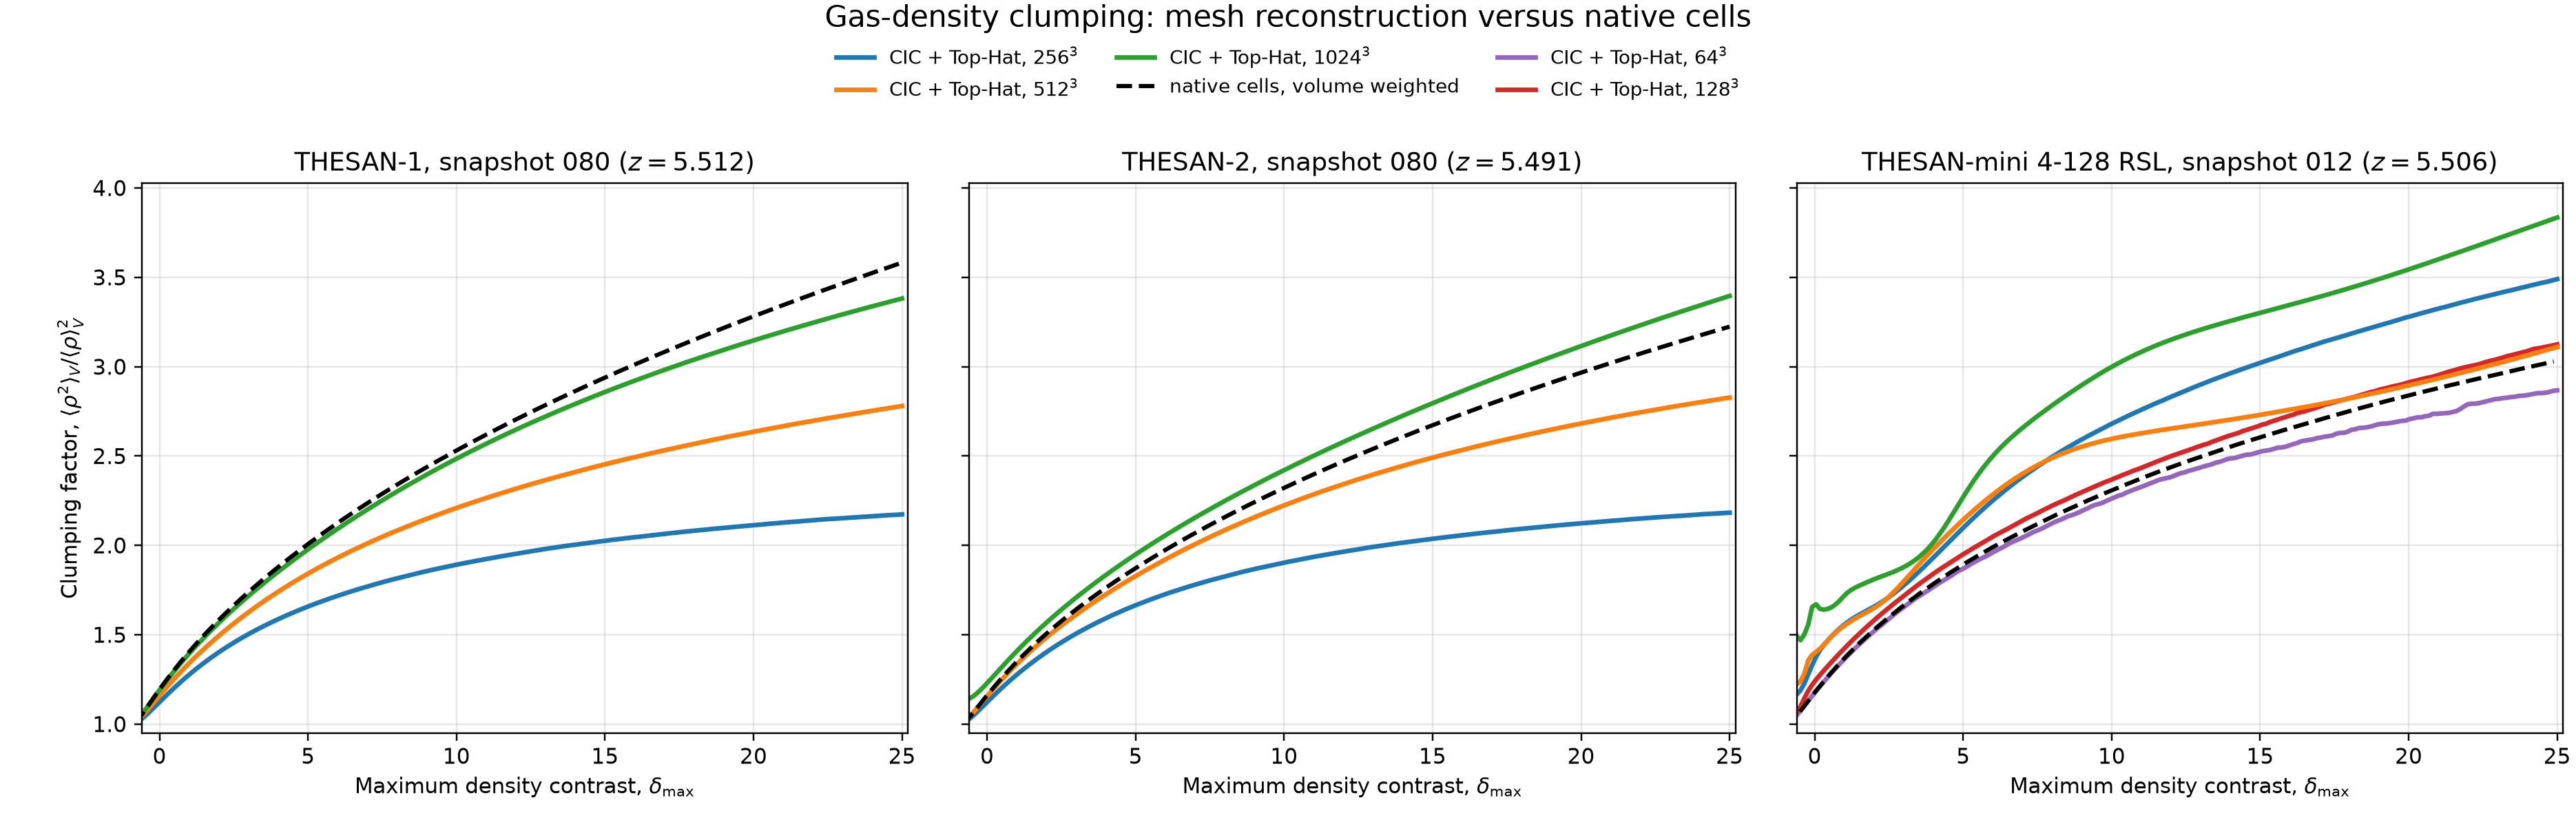
\includegraphics[width=1\textwidth]{figures/thesan_grid_native_mini.png}
    \caption{Clumping factor computation at different grid sizes as a function of overdensity compared to the Voronoi-cell direct computation. Left: Thesan-1 simulation; Center: Thesan-2 simulation; Right: Thesan-mini\footnote{Thesan-mini corresponds to a $128^3$ particles 4 Mpc simulation with the same conditions and software as the Thesan simulations that was run for this project. \label{fn:Thesan-mini}}  }
    \label{fig:grid-size_comparison_thesan}
\end{figure*}

The first comparison that comes to mind is to compare the clumping factor for different grid sizes with respect to a more direct implementation using the Voronoi cells. In Figure \ref{fig:grid-size_comparison_thesan} we have such a comparison. The first important realizationi from this Figure is the fact that the relation of the gridded clumping factor to the native cell calculation depends not so much on the grid size $g$ but rather the factor gridding factor $g/N$ with $N$ being the linear density of initial particles (that is, the full simulation has $N^3$ particles). We note that Thesan-1 has $N=2100$, Thesan-2 has $N=1050$ and Thesan-mini\footref{fn:Thesan-mini} has $N=128$. 

Thus, we note that when $g/N \approx 1$ the gridded calculation slightly overestimates the native calculation but follows the tendency fairly accurately while for $g/N \approx 0.5$ the gridded calculation gives a slighly smaller result but also tends to follow the tendency fairly accurately until higher overdensity thresholds. 

Moreover, in the Thesan-mini calculations one can observe that using a grid size too fine with respect to the number of particles introduces some instabilities that the smoothing and cloud in cell assignment aren't able to eliminate. 

This comparison is extremely informative, however, it only explores the data as a singular redshift. Therefore, we would like to see if similar behaviors hold for different redshifts. In order to carry out this comparison, let us define a gridding-deviation measure as follows:
$$\Delta_{grid} = \int_0^{25} \frac{C_{Voronoi} - C_{grid}}{C_{Voronoi}} d\delta,$$
where $C_{Voronoi}$ corresponds to the clumping factor calculated using the native cells, and $C_{grid}$ to the calculation at a given grid size. Thus, we can see this comparison in Figure \ref{fig:gridding_deviation_factor_Thesan-2} that earlier in the simulation a gridding factor close to unity almost exactly matches the native calculation, this corresponds to a lower clumping factor overall and thus the Voronoi cell sizes being more uniform throughout the simulation space. However, as the simulation progresses and the halos collapse the finer grid size starts to overestimate the clumping factor where as smaller grids get closer to it. 

\begin{figure}
    \centering
    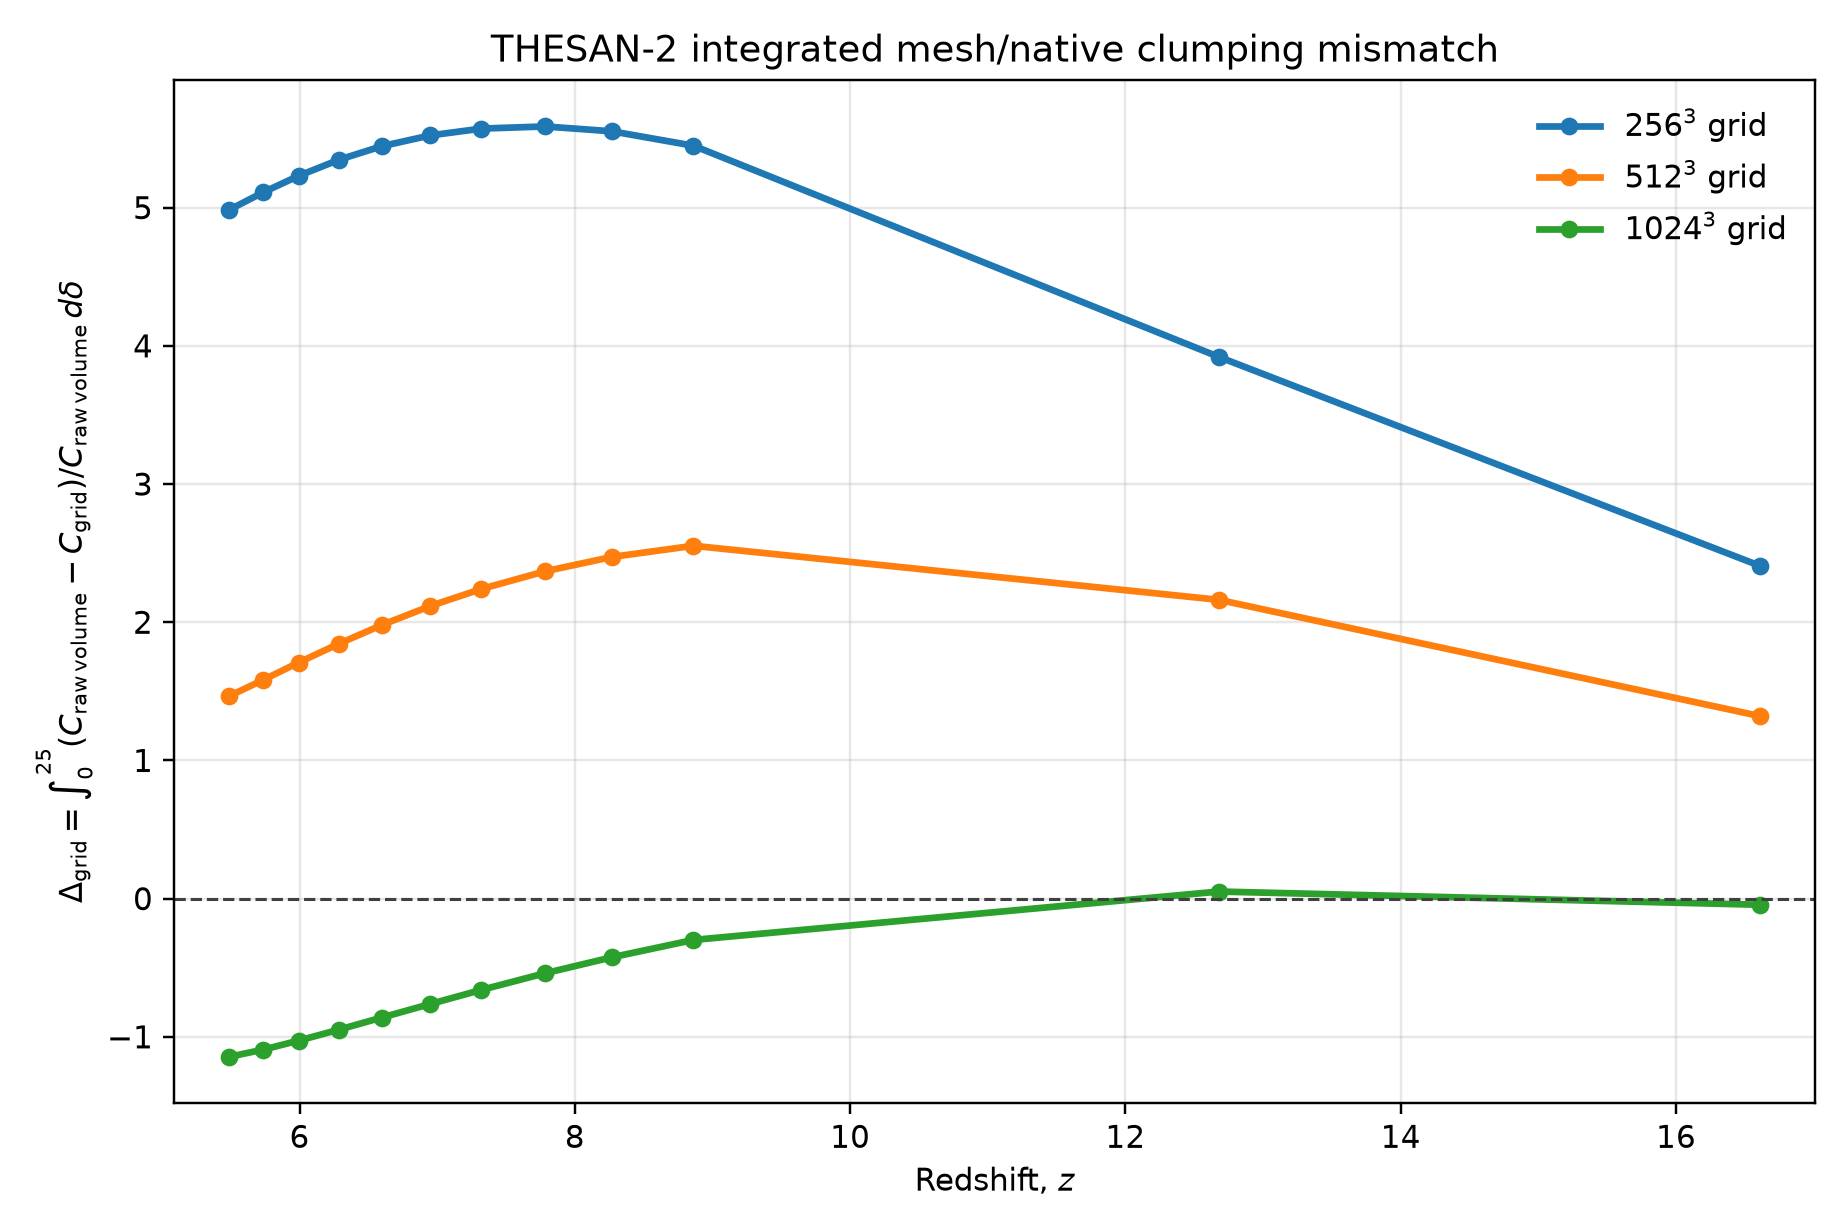
\includegraphics[width=1\linewidth]{figures/delta_grid_vs_redshift.png}
    \caption{Gridding deviation at different grid sizes as a function of redshift for Thesan-2}
    \label{fig:gridding_deviation_factor_Thesan-2}
\end{figure}

Similar tests for the AIDA-TNG simulations were run and are included in the appendix \ref{apx:AIDA-TNG}. In the end for most of the results presented in this report we will use a gridding factor of 0.5, this choice was taken both because it matches our results considerably well and for computationally efficiency as both memory usage and computation time depend on the cube of the grid size (before implmenting multithreading).

Thus, having taken this choice the smoothing backend becomes way less important considering that for such a gridding factor for a particle to be smoothed their effective size would have to be larger than twice the interparticle distance which is very rare considering this corresponds to having an average density of 8 times less than the average particle. As we can see in Figure \ref{fig:smoothing-techniques}, for Thesan-2 with a grid of 1024 which corresponds to a griddind factor close to unity we cannot observe the differences between the different smoothing methods. Therefore, we choose to use Pylians as our backend since it is an established library and allows us to easily implement cloud in cell as part of this mass assignment process. 

\begin{figure}
    \centering
    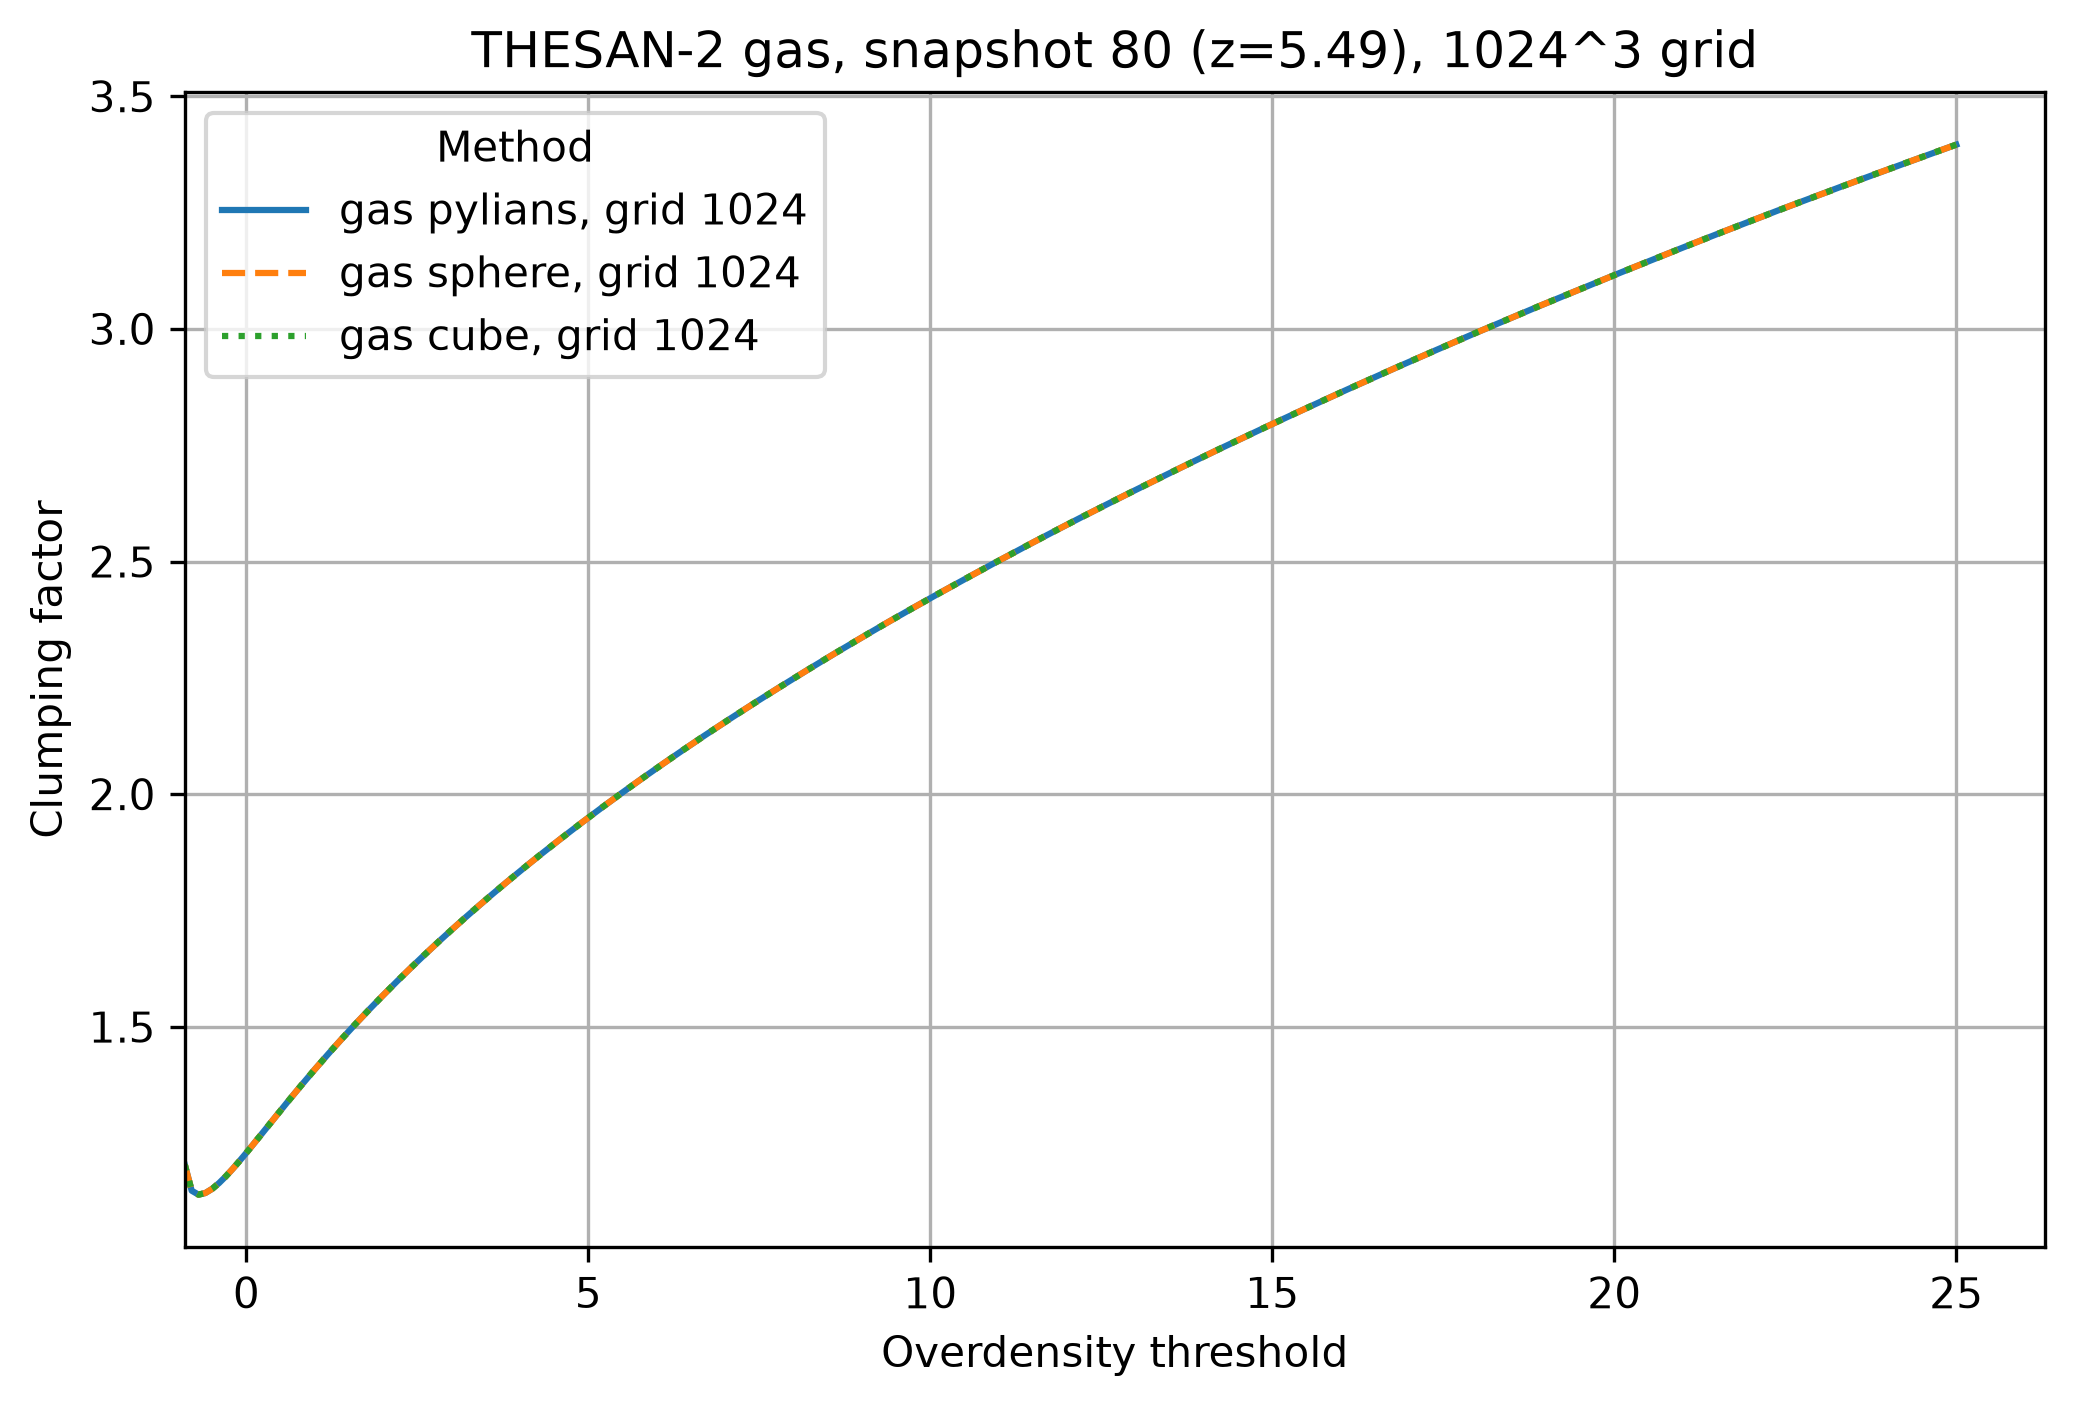
\includegraphics[width=1\linewidth]{figures/thesan2-1024-smoothing-codebase.png}
    \caption{Comparison of different smoothing techniques in the calculation of the clumping factor as a function of overdensity for Thesan 2}
    \label{fig:smoothing-techniques}
\end{figure}

The case for dark matter is slightly more nuanced than that for gas, in most of the computations present in this work we have used the interparticle distance as a universal particle size for dark matter. Therefore, no smoothing will be carried out for a gridding factor of less than unity. However, the simulations treated in this work do include a subfindhml figure that can be used as a proxy for the size of our particles, the effects of this while not present in the main body of the report can be seen in the appendix \ref{apx:AIDA-TNG} mentioned earlier.

\subsection{Dependence on the IGM definition}
As observed in the previous figures the clumping factor has a very strong dependence on the overdensity threshold used to define the IGM. Therefore, in this work we are not going to assess which values specifically should be used but rather present most of our work as a function of overdensity and use this as our only cutoff for the defition of the IGM. 

The only exception will be the comparison against other estimators of Section \ref{sec:appl1} where some of the assumptions of these estimators will include ionization equilibrium. Thus, we will use an extra cutoff, one on the ionized fraction of our cells, to guarantee that the sections of the IGM we include in our calculations satisfy this assumption properly. 

\subsection{Power spectrum consistency tests}
As mentioned in the methodology section, we have two different backends implemented for the calculation of the power spectrum. In this section we will compare these two backends and see how they differ in the high k region where the gridding generates numerical artifacts. After this we will compare them with the results obtained by the arepo implementation and validate with it the folding procedure. Lastly we will validate our calculations for the different dark matter models against the results from the AIDA-TNG paper.

In Figure \ref{fig:numpy-pylians_parity} we can observe that both backends give us very similar results for one of the particular AIDA-TNG simulations. Indeed, the main difference is observed between grid sizes for which the finer grid sizes allow us to explore higher k sections before the power spectrum starts to decrease.  

This decrease at high (k) is expected. The cloud-in-cell (CIC) mass-assignment scheme distributes the mass of each particle over neighbouring grid cells, which has the effect of  smoothing the density field on scales comparable to the grid-cell size. As a consequence, the power spectrum of the corresponding Fourier modes is suppressed with respect to that of a continuous density field.

\begin{figure}
    \centering
    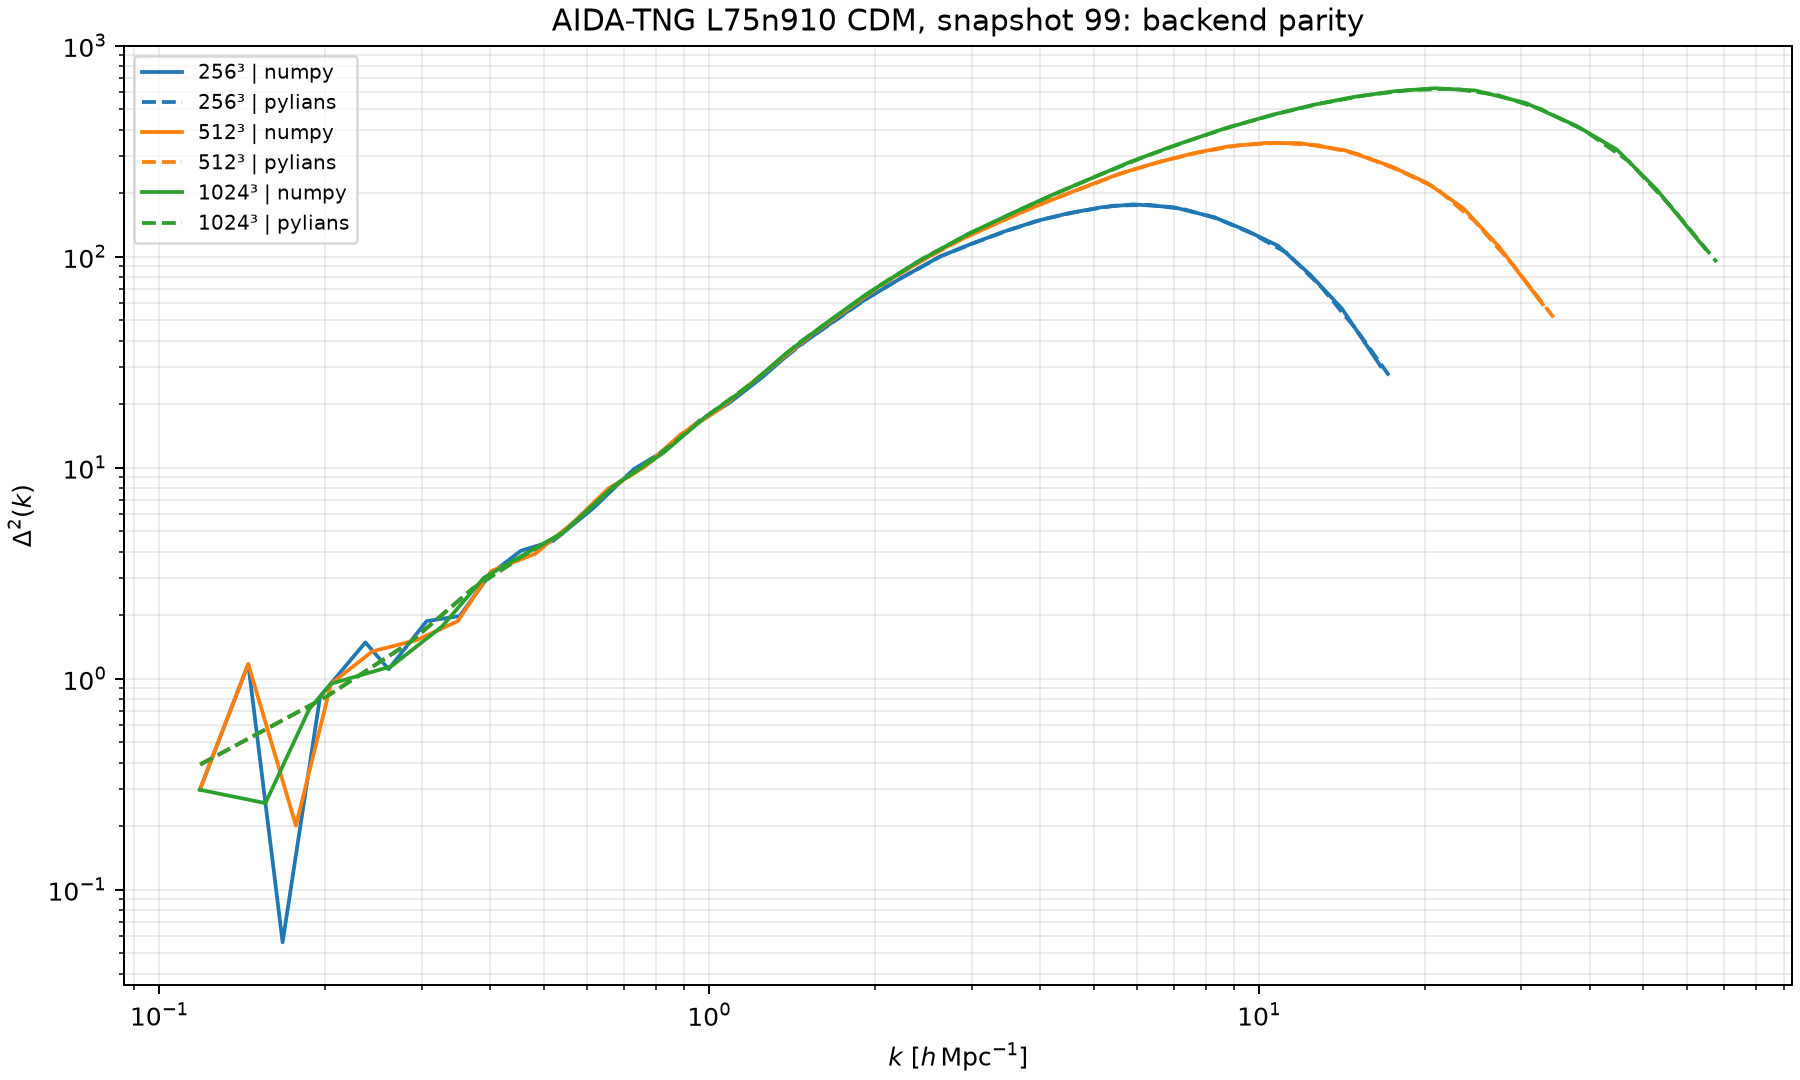
\includegraphics[width=1\linewidth]{figures/l75n910-cdm-fold1-backend-parity.png}
    \caption{Comparison of the calculation of the power spectrum of AIDA-TNG L75n910 CDM simulation at redishift 0 for the different backends and different grid sizes}

        \label{fig:numpy-pylians_parity}
\end{figure}
Pylians also provides a built-in correction for the CIC mass-assignment window. We show the effect of this correction in Figure \ref{fig:numpy-pylians-correction}. This procedure approximately divides the measured power spectrum by the suppression factor introduced by CIC. At high (k), however, this factor becomes small. The correction then amplifies not only the suppressed power spectrum, but also noise and aliasing effects. This is why the corrected Pylians spectra begin to diverge close to the grid scale.

\begin{figure}
        \centering
        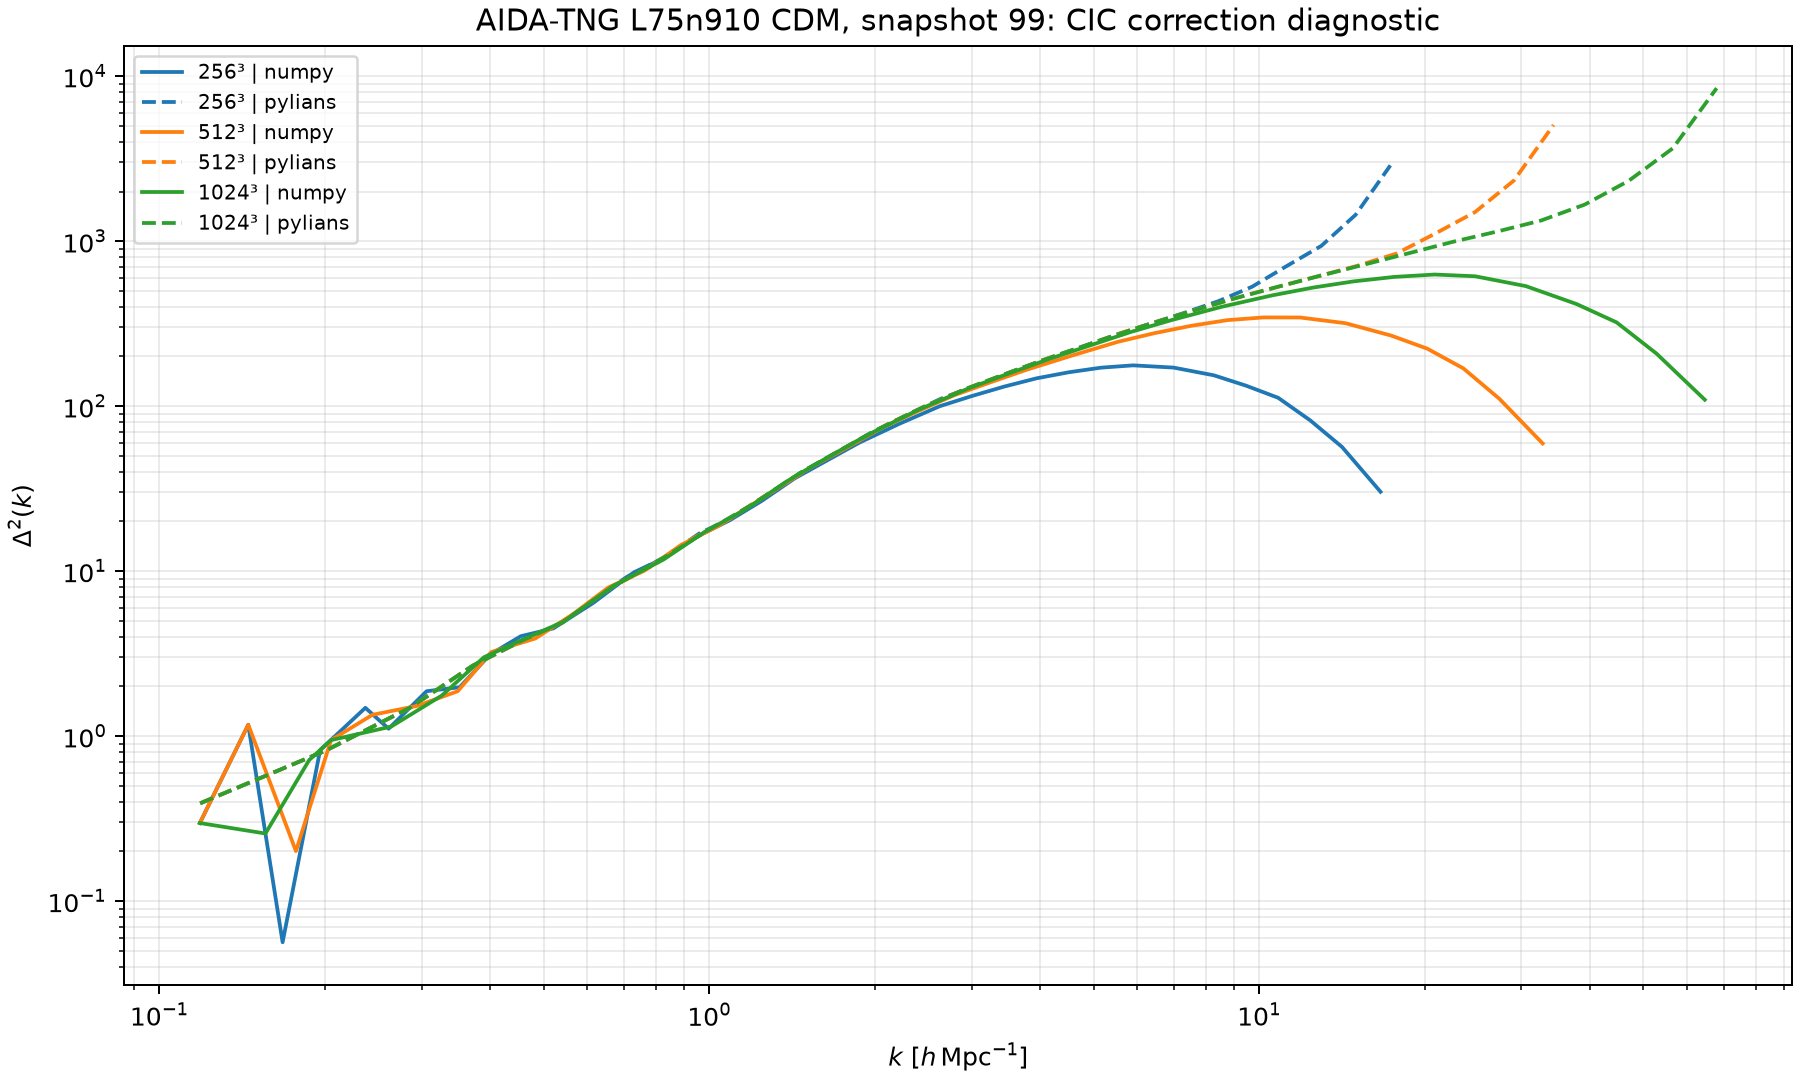
\includegraphics[width=1\linewidth]{figures/l75n910-cdm-fold1-mas-correction.png}
        \caption{Effect of the cloud-in-cell correction functionality of the Pylians library}
        \label{fig:numpy-pylians-correction}
    \end{figure}





In order to validate our implementation, we compare the spectra with those produced by the built-in power-spectrum calculator in the AREPO simulation software used to run AIDA-TNG. The AREPO output contains three blocks, a direct calculation and two folded spectra corresponding to $f=1$, $16$, and $256$. Our $1024^3$ Pylians calculation uses the same folding factors and the added cloud-in-cell correction. We can see this comparison in Figure \ref{fig:pylians-arepo} where the upper panel shows the absolute spectra and the lower panel shows the ratio between the two implementations. We can observe that they agree closely in their overlapping ranges. The Pylians spectra extend beyond the AREPO ranges because we are using a finer grid for the calculation, however, these extensions should be treated with caution as the cloud-in-cell correction amplifies aliasing and noise at high $k$.

\begin{figure}
    \centering
    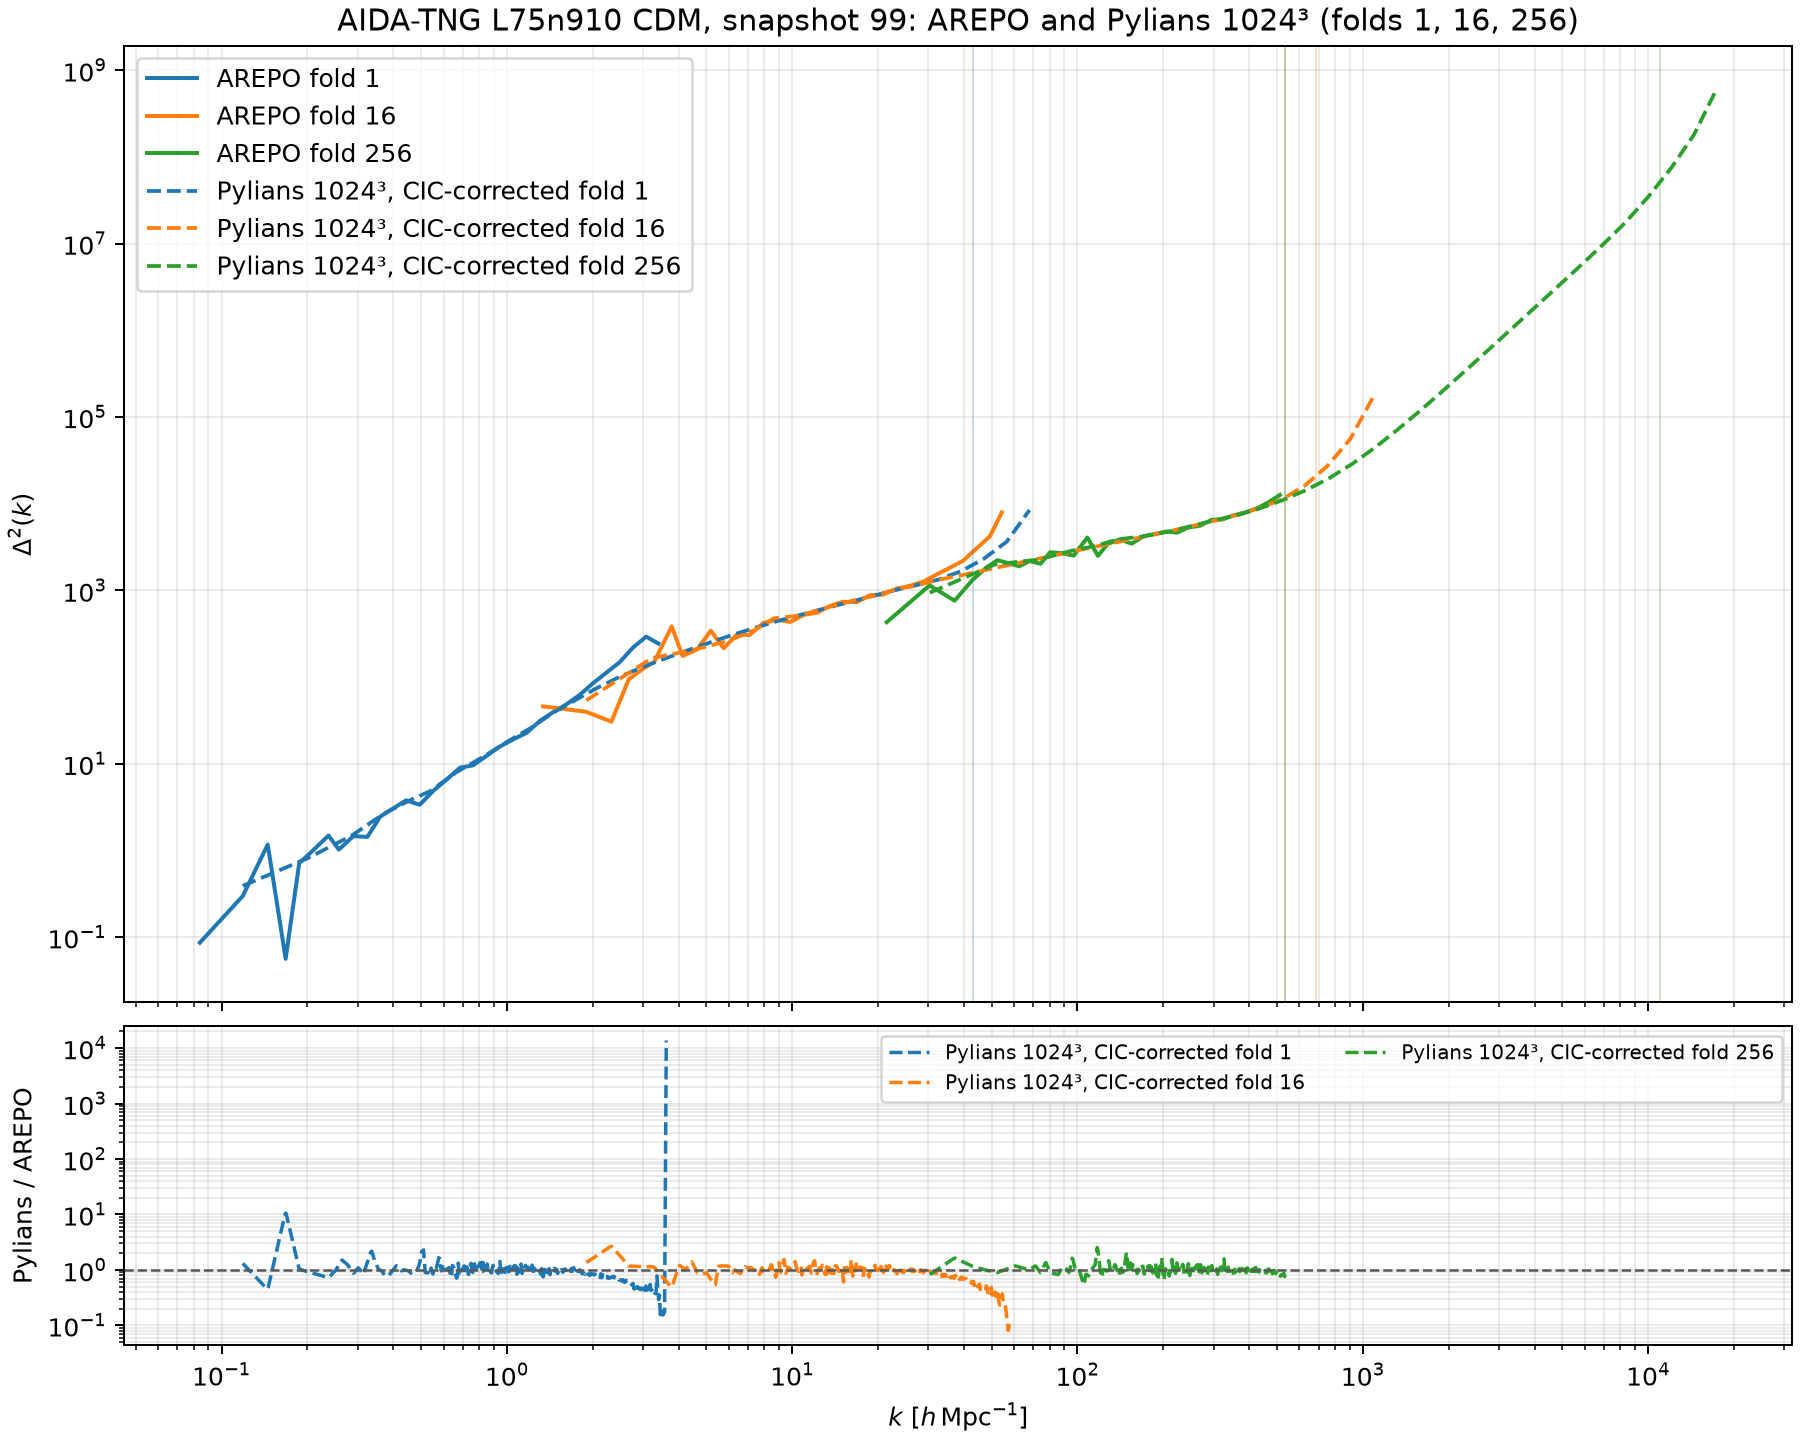
\includegraphics[width=1\linewidth]{figures/l75n910-cdm-grid1024-pylians-vs-arepo-folds.png}
    \caption{Dimensionless dark-matter power spectra for the AIDA-TNG L75n910 CDM simulation at snapshot 99. Solid curves show the AREPO measurements and dashed curves show the cloud-in-celll corrected Pylians $1024^3$ grid calculation. Colours identify the folding factors $f=1$, $16$, and $256$; the lower panel shows the Pylians-to-AREPO ratio over the overlapping ranges.}
    \label{fig:pylians-arepo}
\end{figure}



... comparison against AIDATNG paper 

\section{Application I: Comparison with Davies et al.}
\label{sec:appl1}

While the clumping factor has a simple formal definition, obtaining a direct observational measurement of the density field of the intergalactic medium is not within the scope of current experiments. Therefore, numerous estimators have been proposed using different assumptions in order to be able to calculate the clumping factor from observationally accessible quantities. Davies et al. \cite{Davies_2026} provide one such approach. In this section, we aim to use our direct clumping factor calculation to compare the different estimators and test the underlying assumptions proposed by Davies et al. in the context of the THESAN simulations. 

\subsection{Reference clumping factor}

In this section we will use as a reference the clumping factor as calculated using the native Voronoi-cells from the simulation. However, for this application we will be interested in the recombination clumping factor coeffcient, which we recall was given by,
$$ C_{rec} \equiv \frac{\left\langle n_e n_{\mathrm{H\,II}} \alpha_{\mathrm{H\,II}} \right\rangle}
{\left\langle n_e \right\rangle
 \left\langle n_{\mathrm{H\,II}} \right\rangle
 \left\langle \alpha_{\mathrm{H\,II}} \right\rangle}.$$ 

This introduces small changes in the calculation, however, for each Voronoi cell in the simulation we have access to the proportion of neutral hydrogen and the electron abudance, thus, these changes only introduce some extra factors into the averages but don't fundamentally change the calculation procedure. Moreover, in all the calculations that follow, we have taken the fiducial recombination coefficient equal to the Case B recombination rate for 10,000K gas. This assumption is matched on the relevant paper. 


\begin{figure}[ht]
    \centering

    \begin{subfigure}{0.48\textwidth}
        \centering
        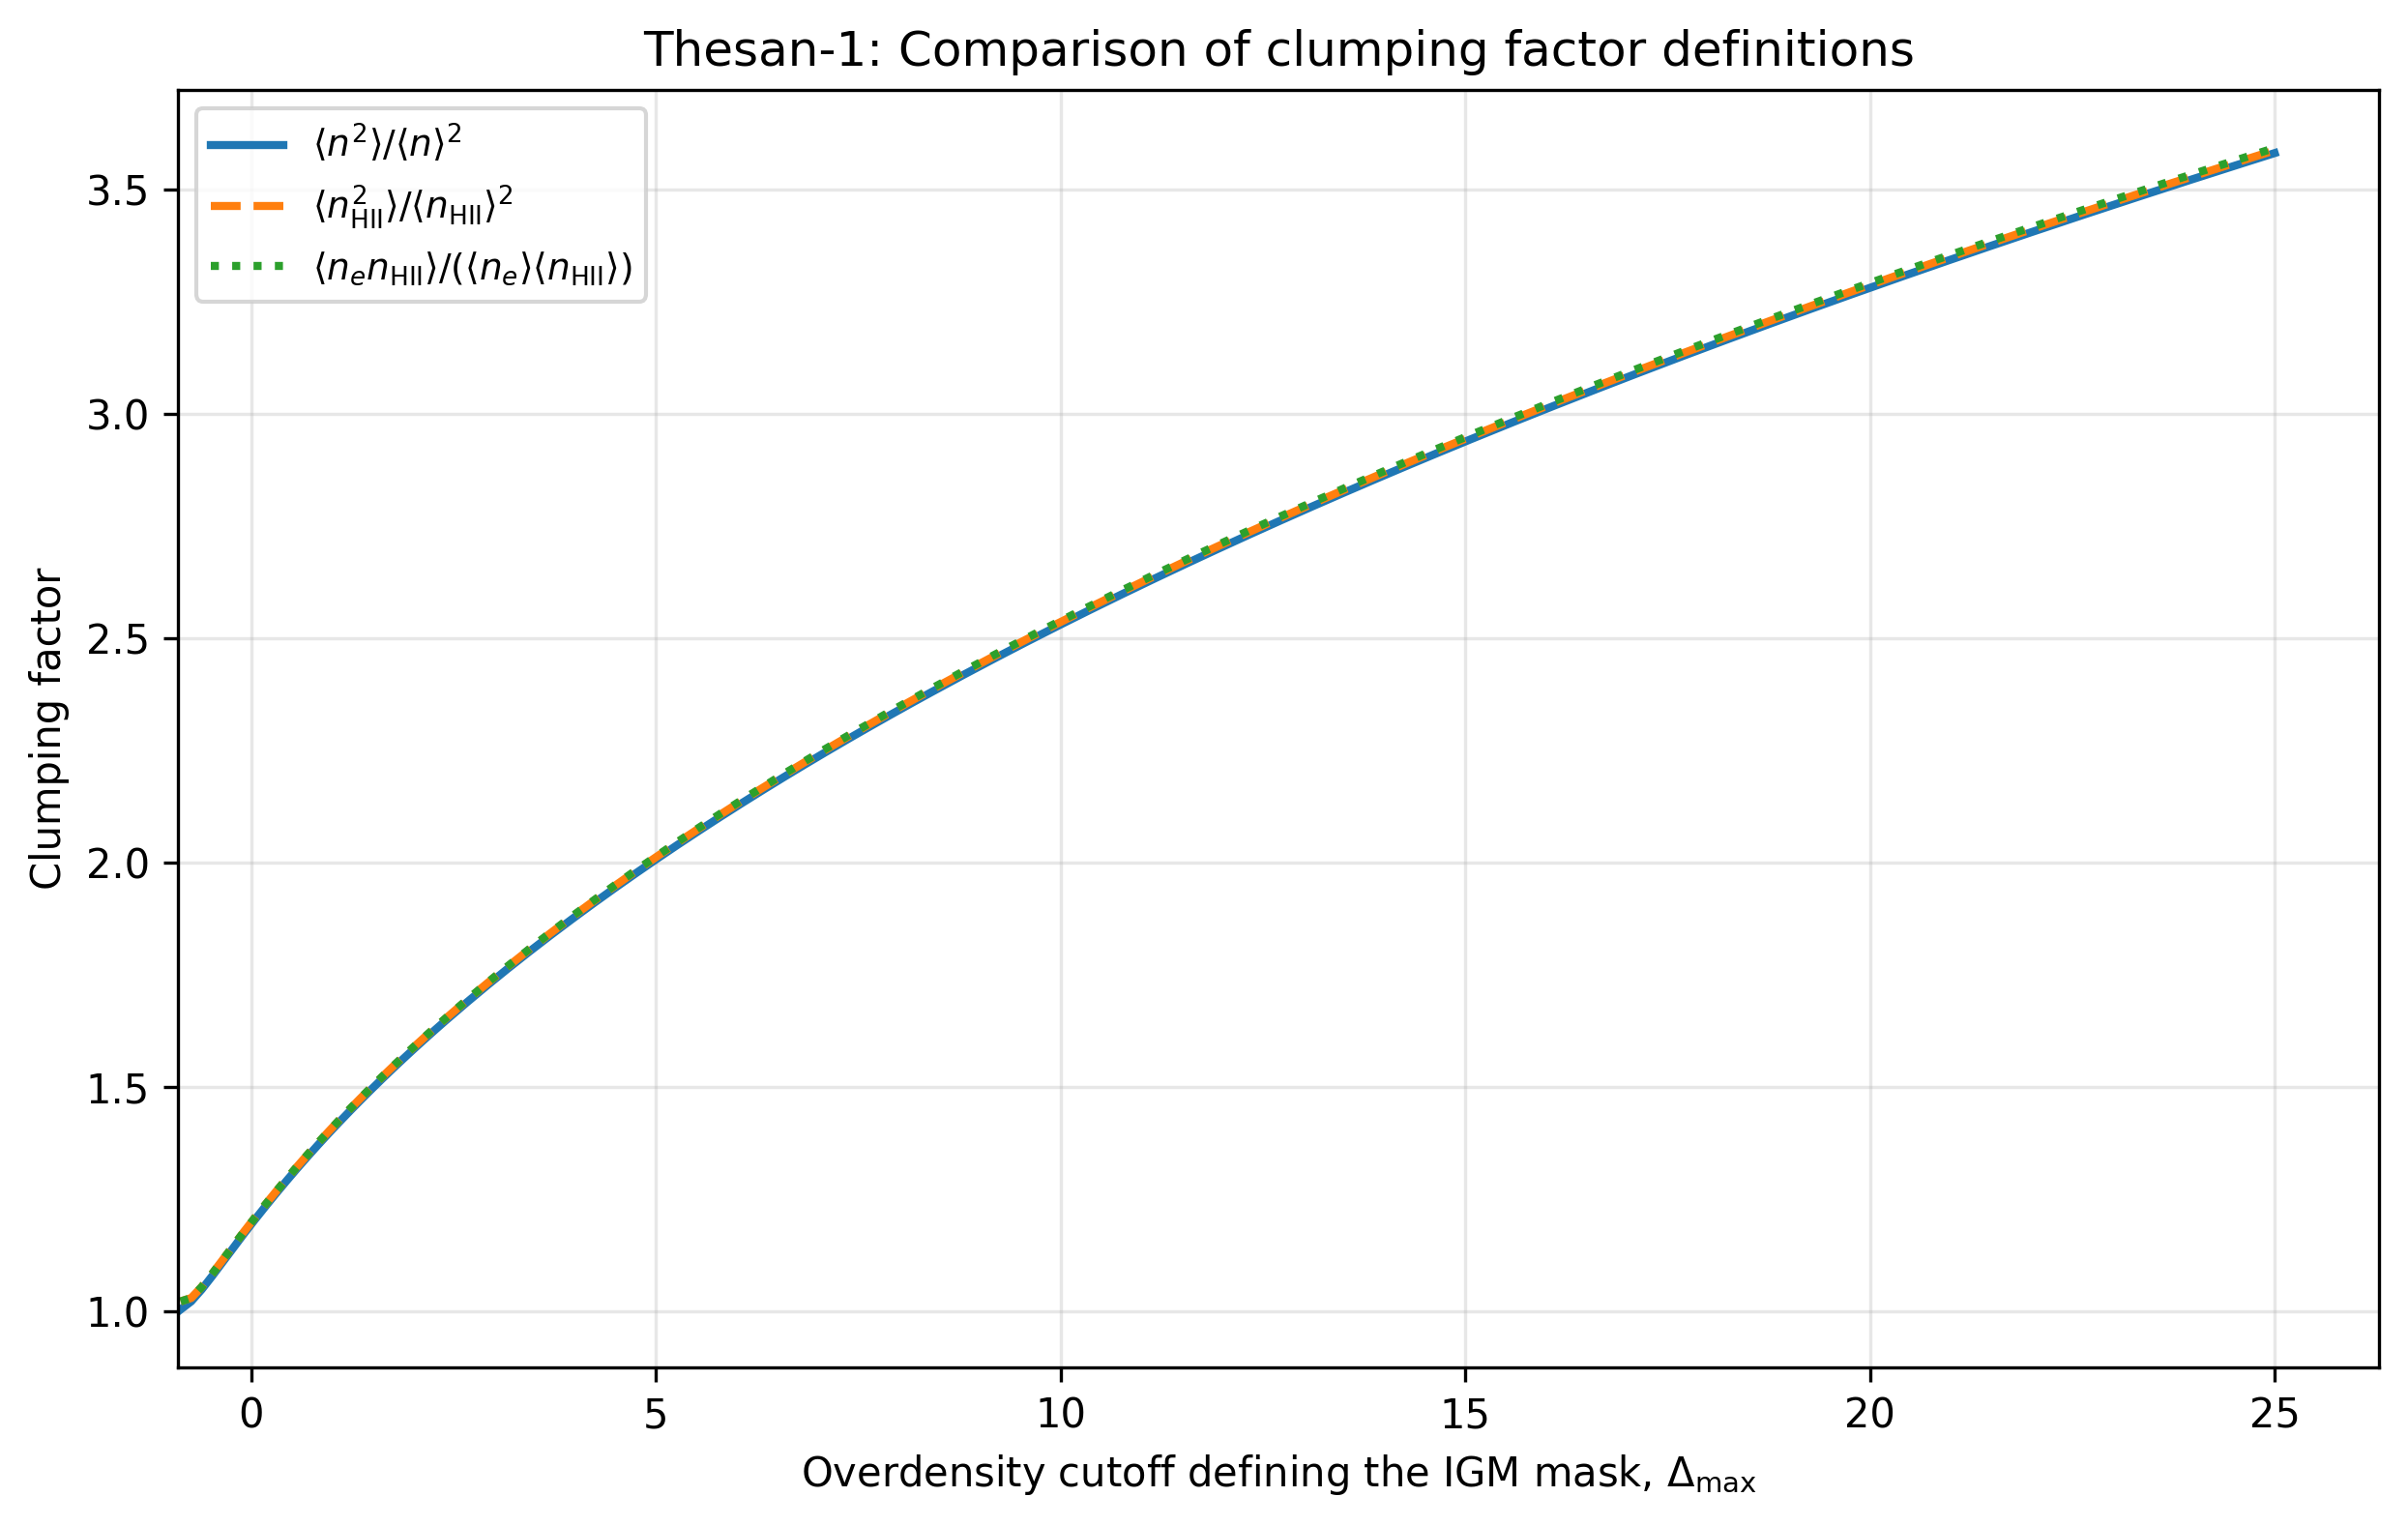
\includegraphics[width=\linewidth]{figures/thesan1_clumping_definitions_snapshot080.png}
    \end{subfigure}
    \hfill
    \begin{subfigure}{0.48\textwidth}
        \centering
        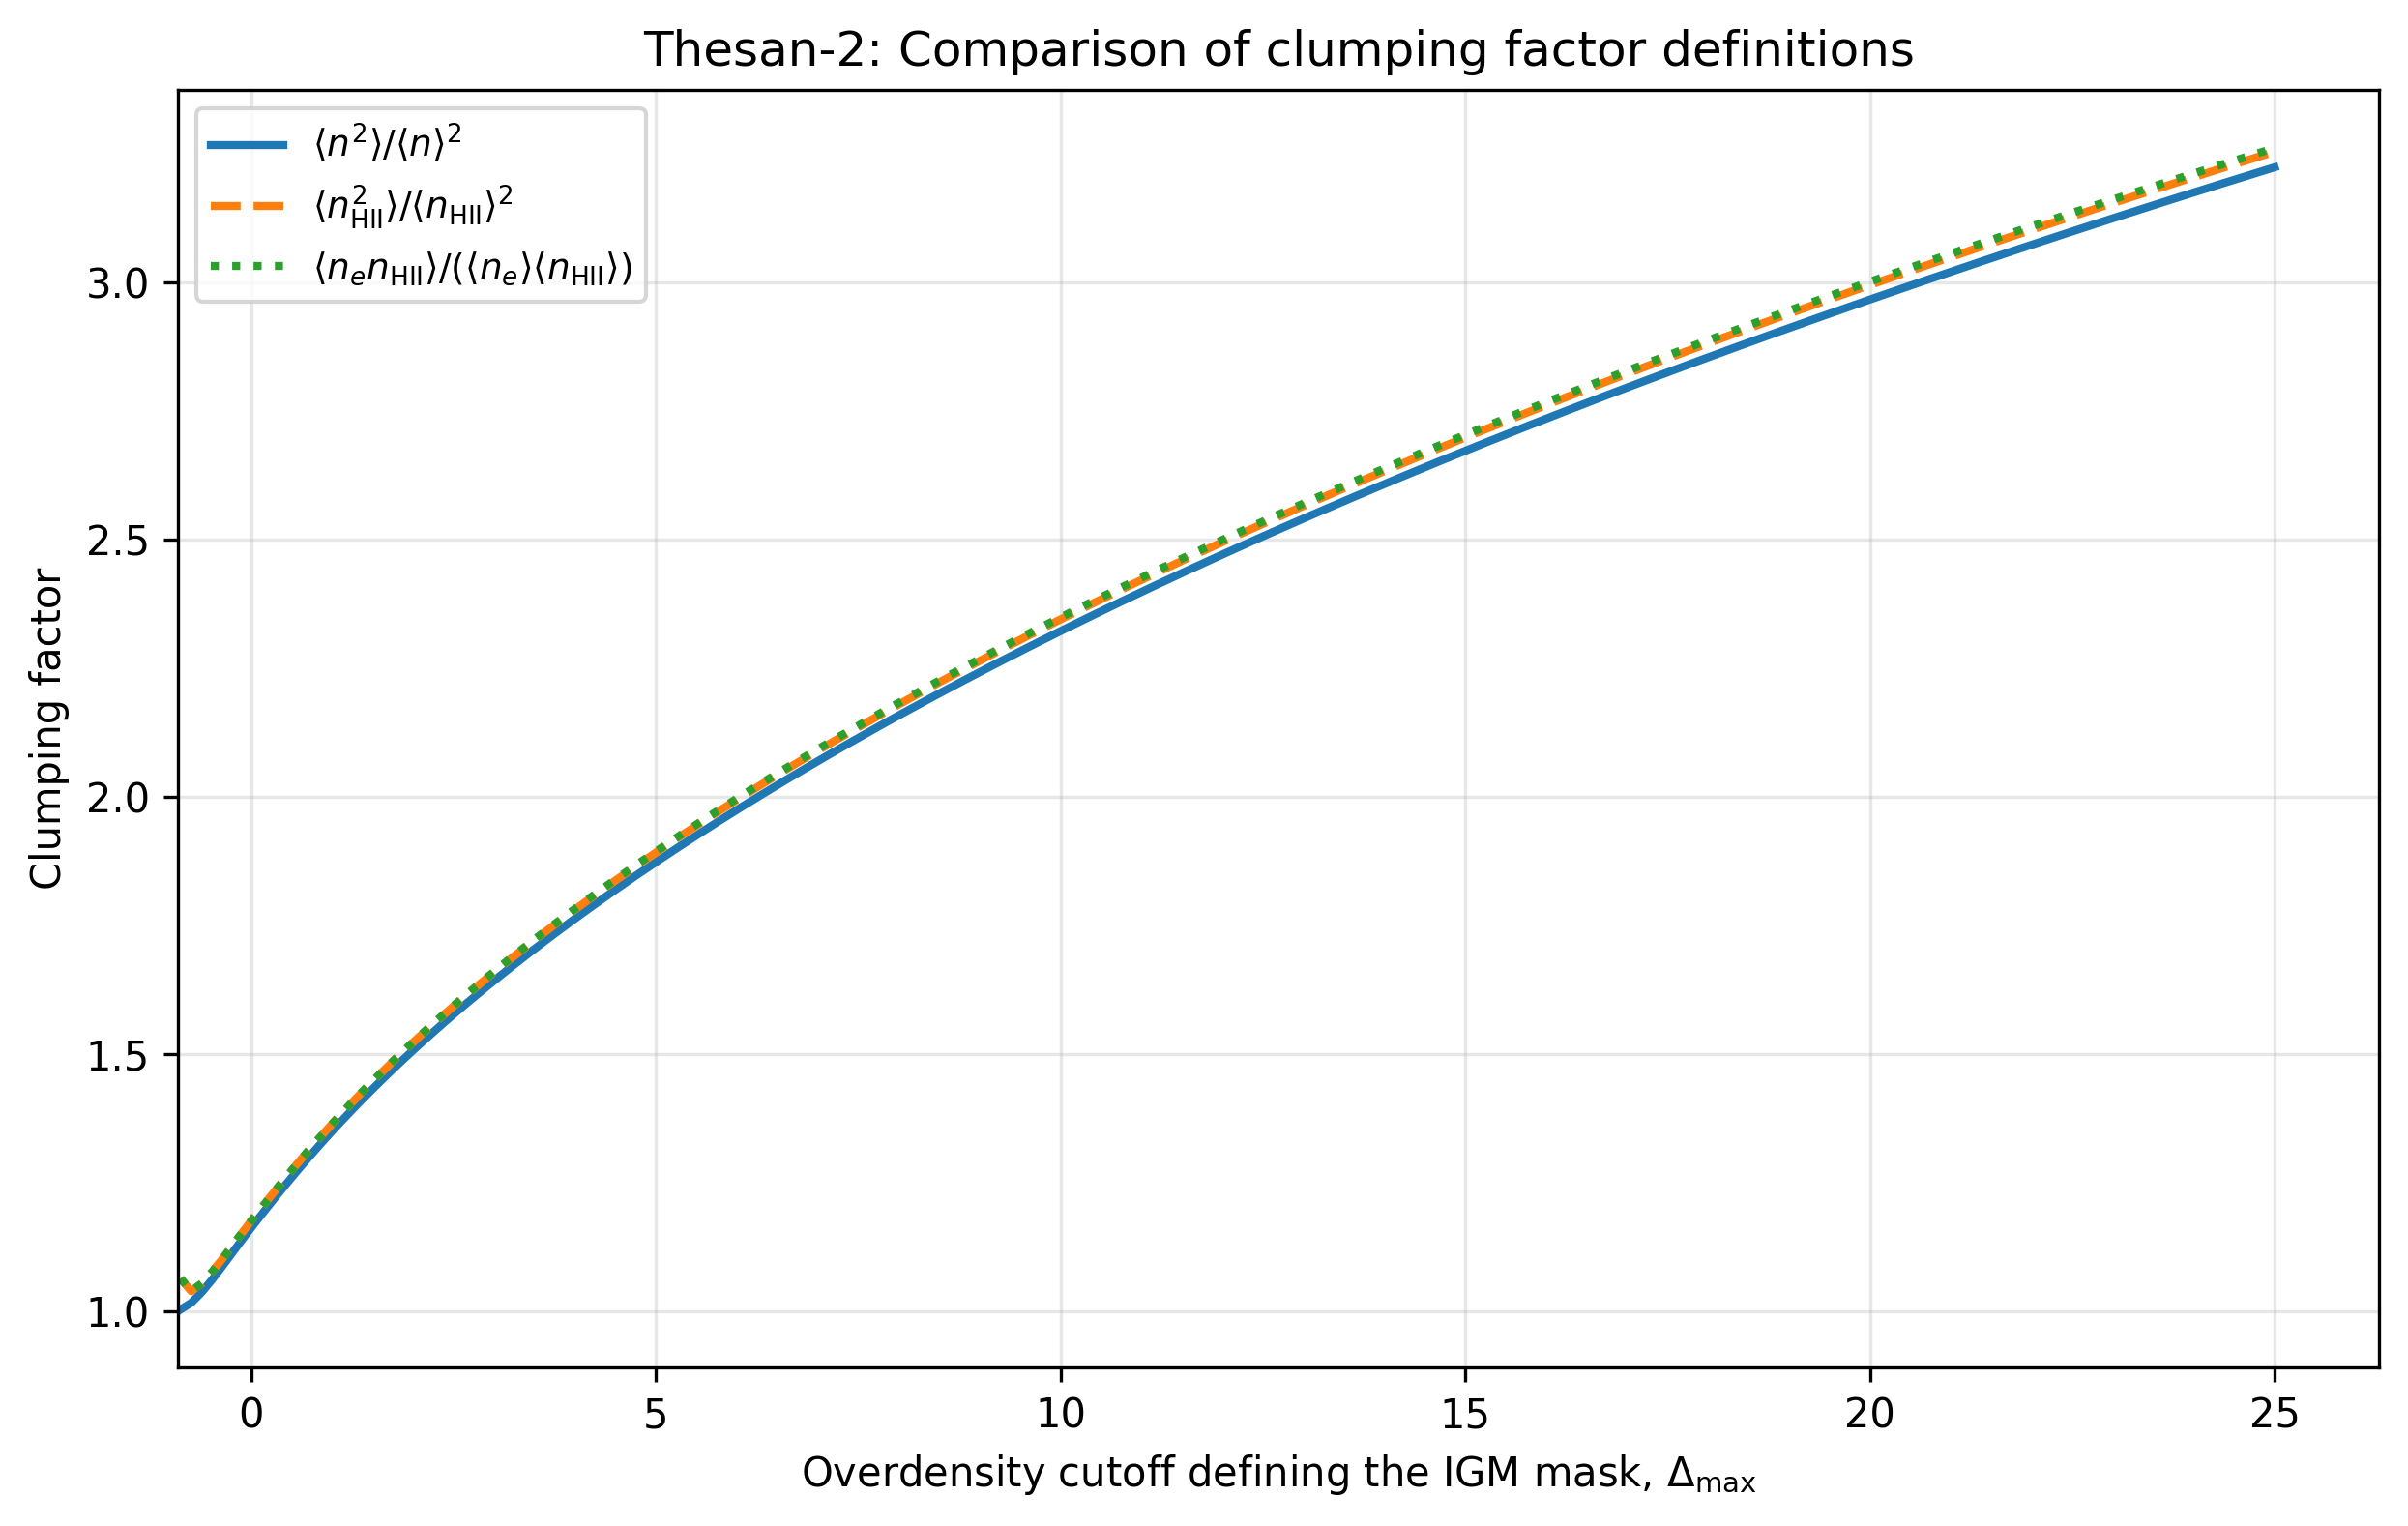
\includegraphics[width=\linewidth]{figures/thesan2_clumping_definitions_snapshot080.png}
    \end{subfigure}

    \caption{Comparison of clumping-factor definitions at snapshot 80. The upper and lower panels show THESAN-1 and THESAN-2, respectively. The curves are plotted as a function of the overdensity cutoff defining the IGM mask.}
    \label{fig:clumping-factor-definitions}
\end{figure}
 

One observes that in Figure.~\ref{fig:clumping-factor-definitions} the changes in the definition only slightly change the obtained results. The difference between the three defintions tested is below $0.36\%$ for THESAN-1 and $1.16\%$ for THESAN-2\footnote{we only have considering the values for $\delta_{\max} \geq 0$ to avoid the artifacts found at $\delta_{\max} \approx -1$.}.

We also note that there is an almost perfect proportionality relationship between $\langle n_{HII} \rangle$ and $\langle n_e \rangle$ of about $\chi_e \approx 1.08$ which matches the value presented by Davies et al to account for the enhancement in the number of free electrons due to ionized helium. 

\begin{figure}
    \centering
    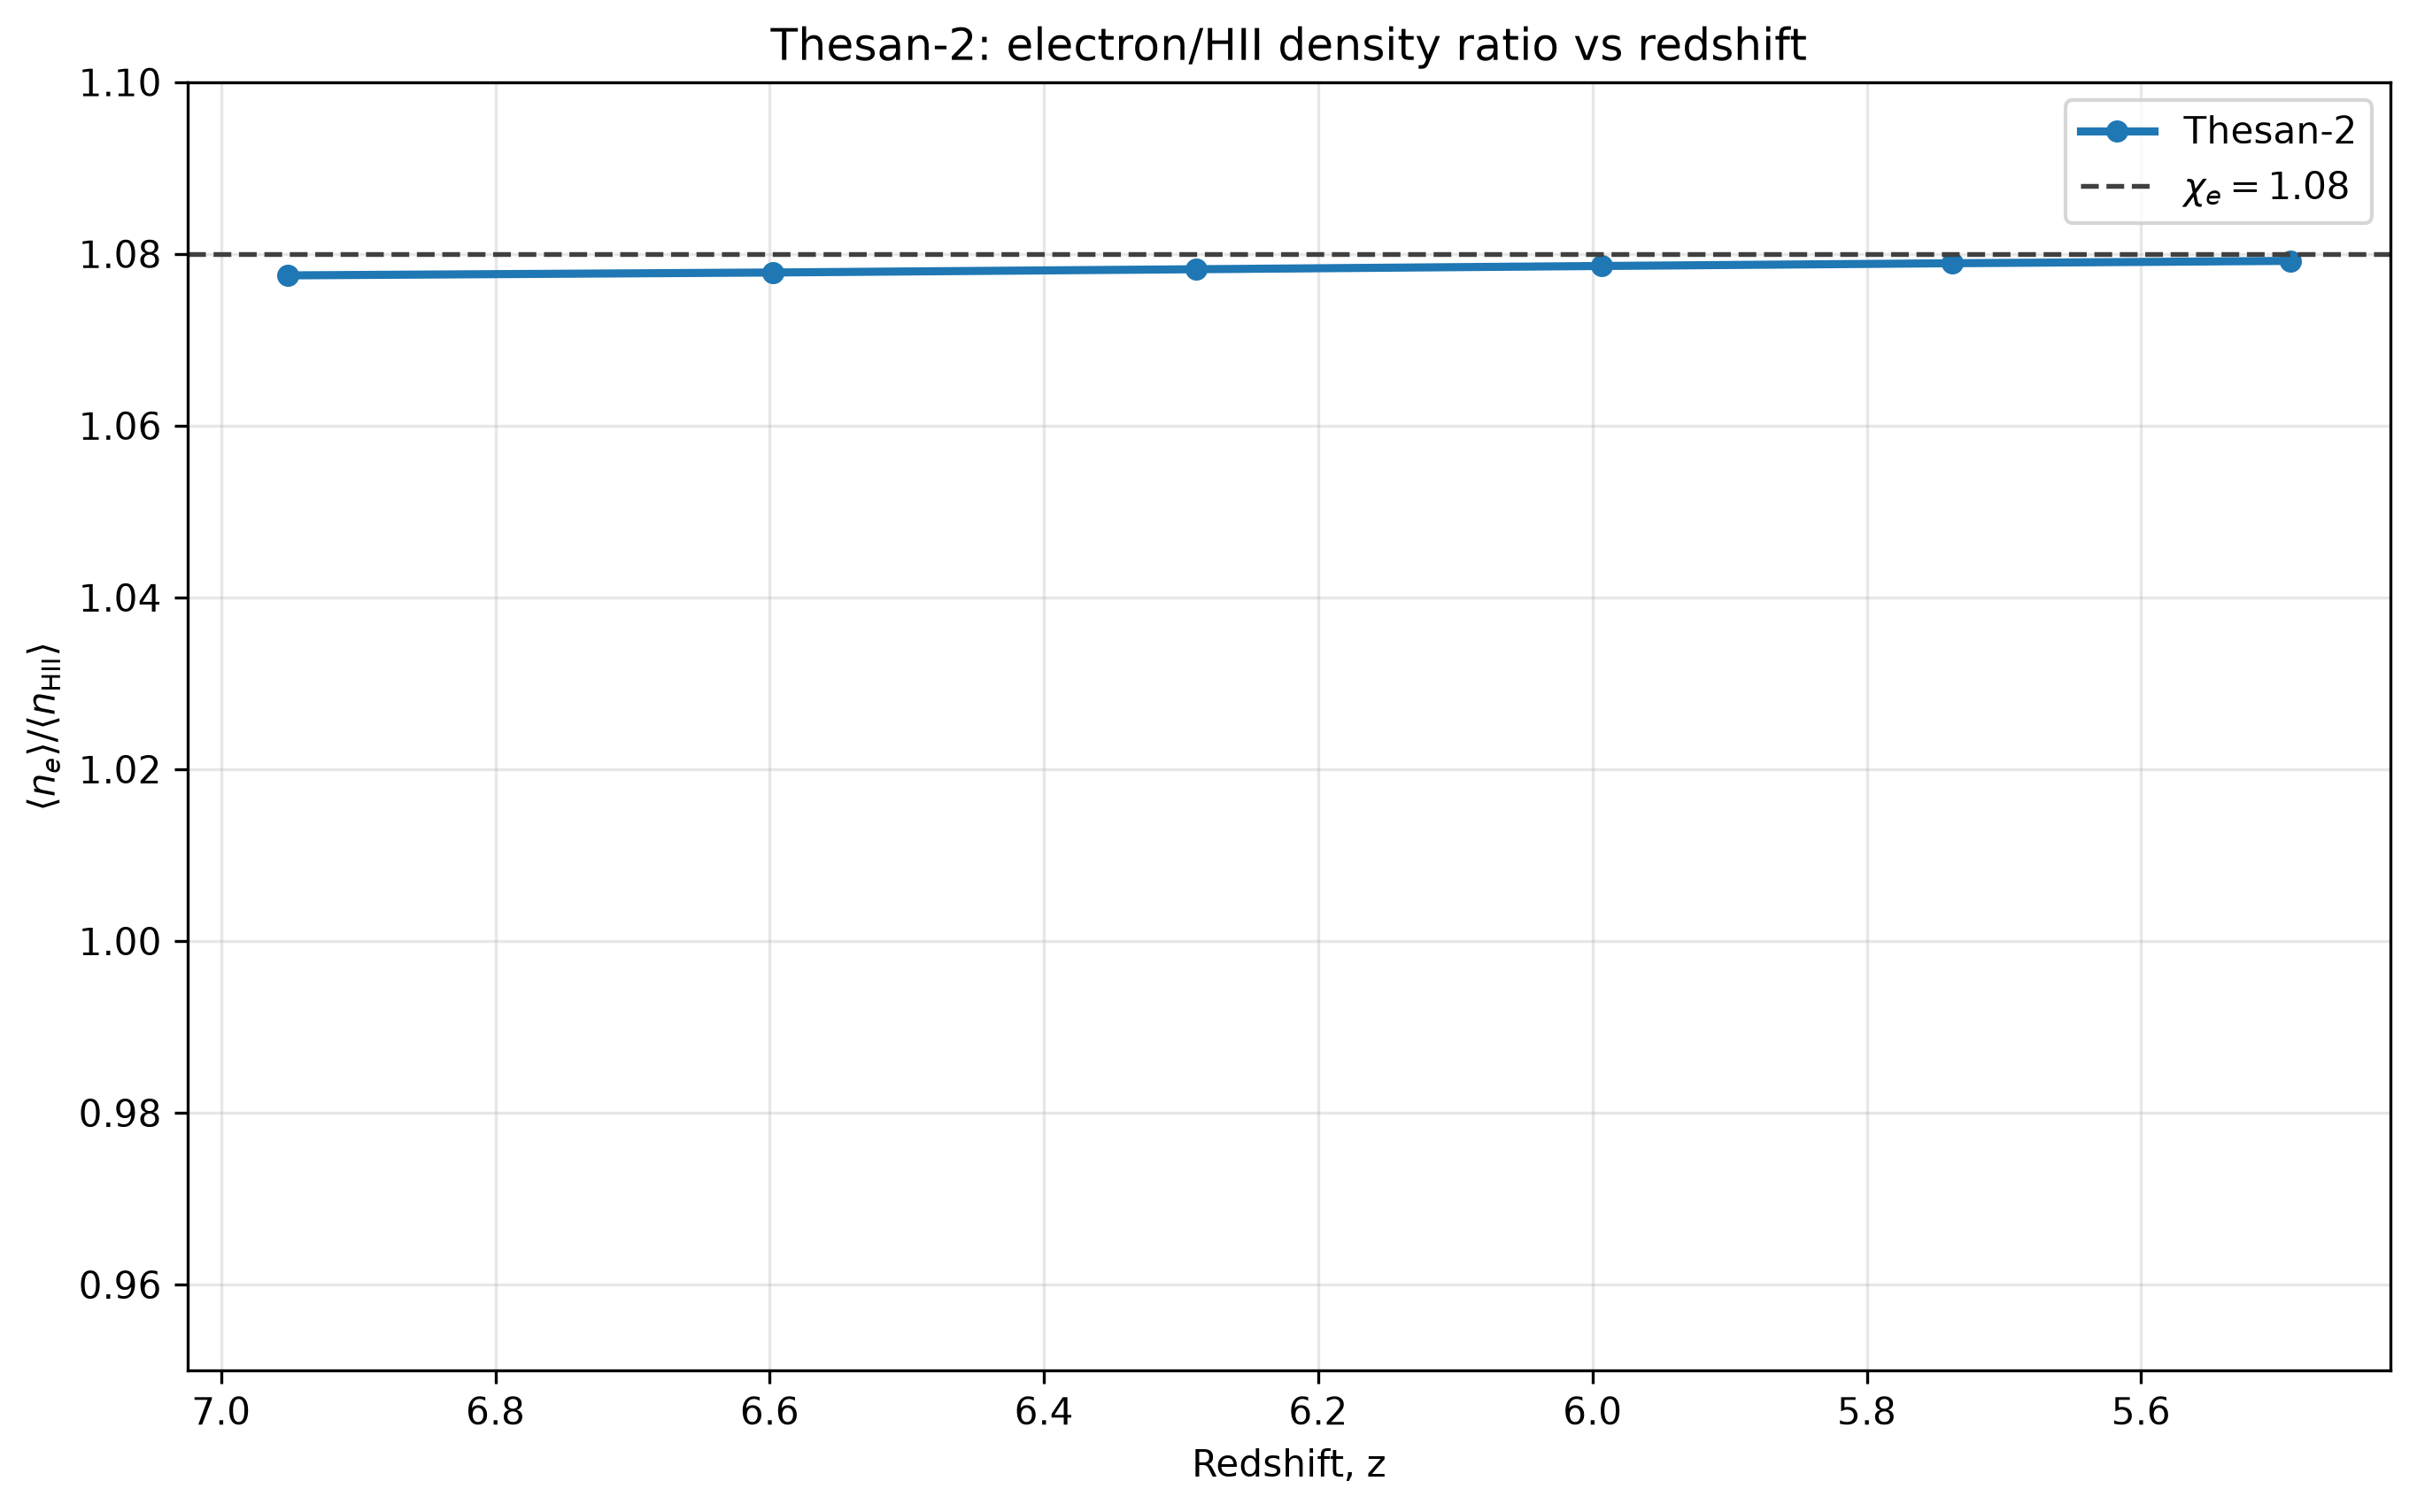
\includegraphics[width=\linewidth]{figures/thesan2_electron_density_ne_over_nHII_vs_redshift_all_gas_chi_e.png}
    \caption{Ratio of free-electron density to ionized-hydrogen density as a function of redshift for all gas in THESAN-2. The approximately constant value supports the use of $\chi_e\simeq1.08$ in the ionized gas.}
    \label{fig:electron-ratio}
\end{figure}

\subsection{Approximate estimator 1: ionization equilibrium}

The first approximate estimator assumes ionization equilibrium.

We make the ionization equilibrium assumption
$$\langle n_{\mathrm{H\,I}} \Gamma_{\mathrm{H\,I}} \rangle
=
\left\langle
n_e n_{\mathrm{H\,II}} \alpha_{\mathrm{H\,II}}
\right\rangle
=
C \chi_e \left(1-x_{\mathrm{H\,I}}\right)^2
n_{\mathrm{H}}^2 \alpha_{\mathrm{H\,II}}$$

which corresponds to 
$$ \langle n_{HI}\Gamma_{HI} \rangle = \langle n_e n_{\mathrm{H\,II}} \alpha_{\mathrm{H\,II}} \rangle$$

Figure~\ref{fig:ionization-equilibrium} shows that the equality is approached only after imposing a more restrictive ionization cut. This is consistent with the presence of neutral islands in the available snapshots, which are taken before the end of reionization.

\begin{figure}
    \centering
    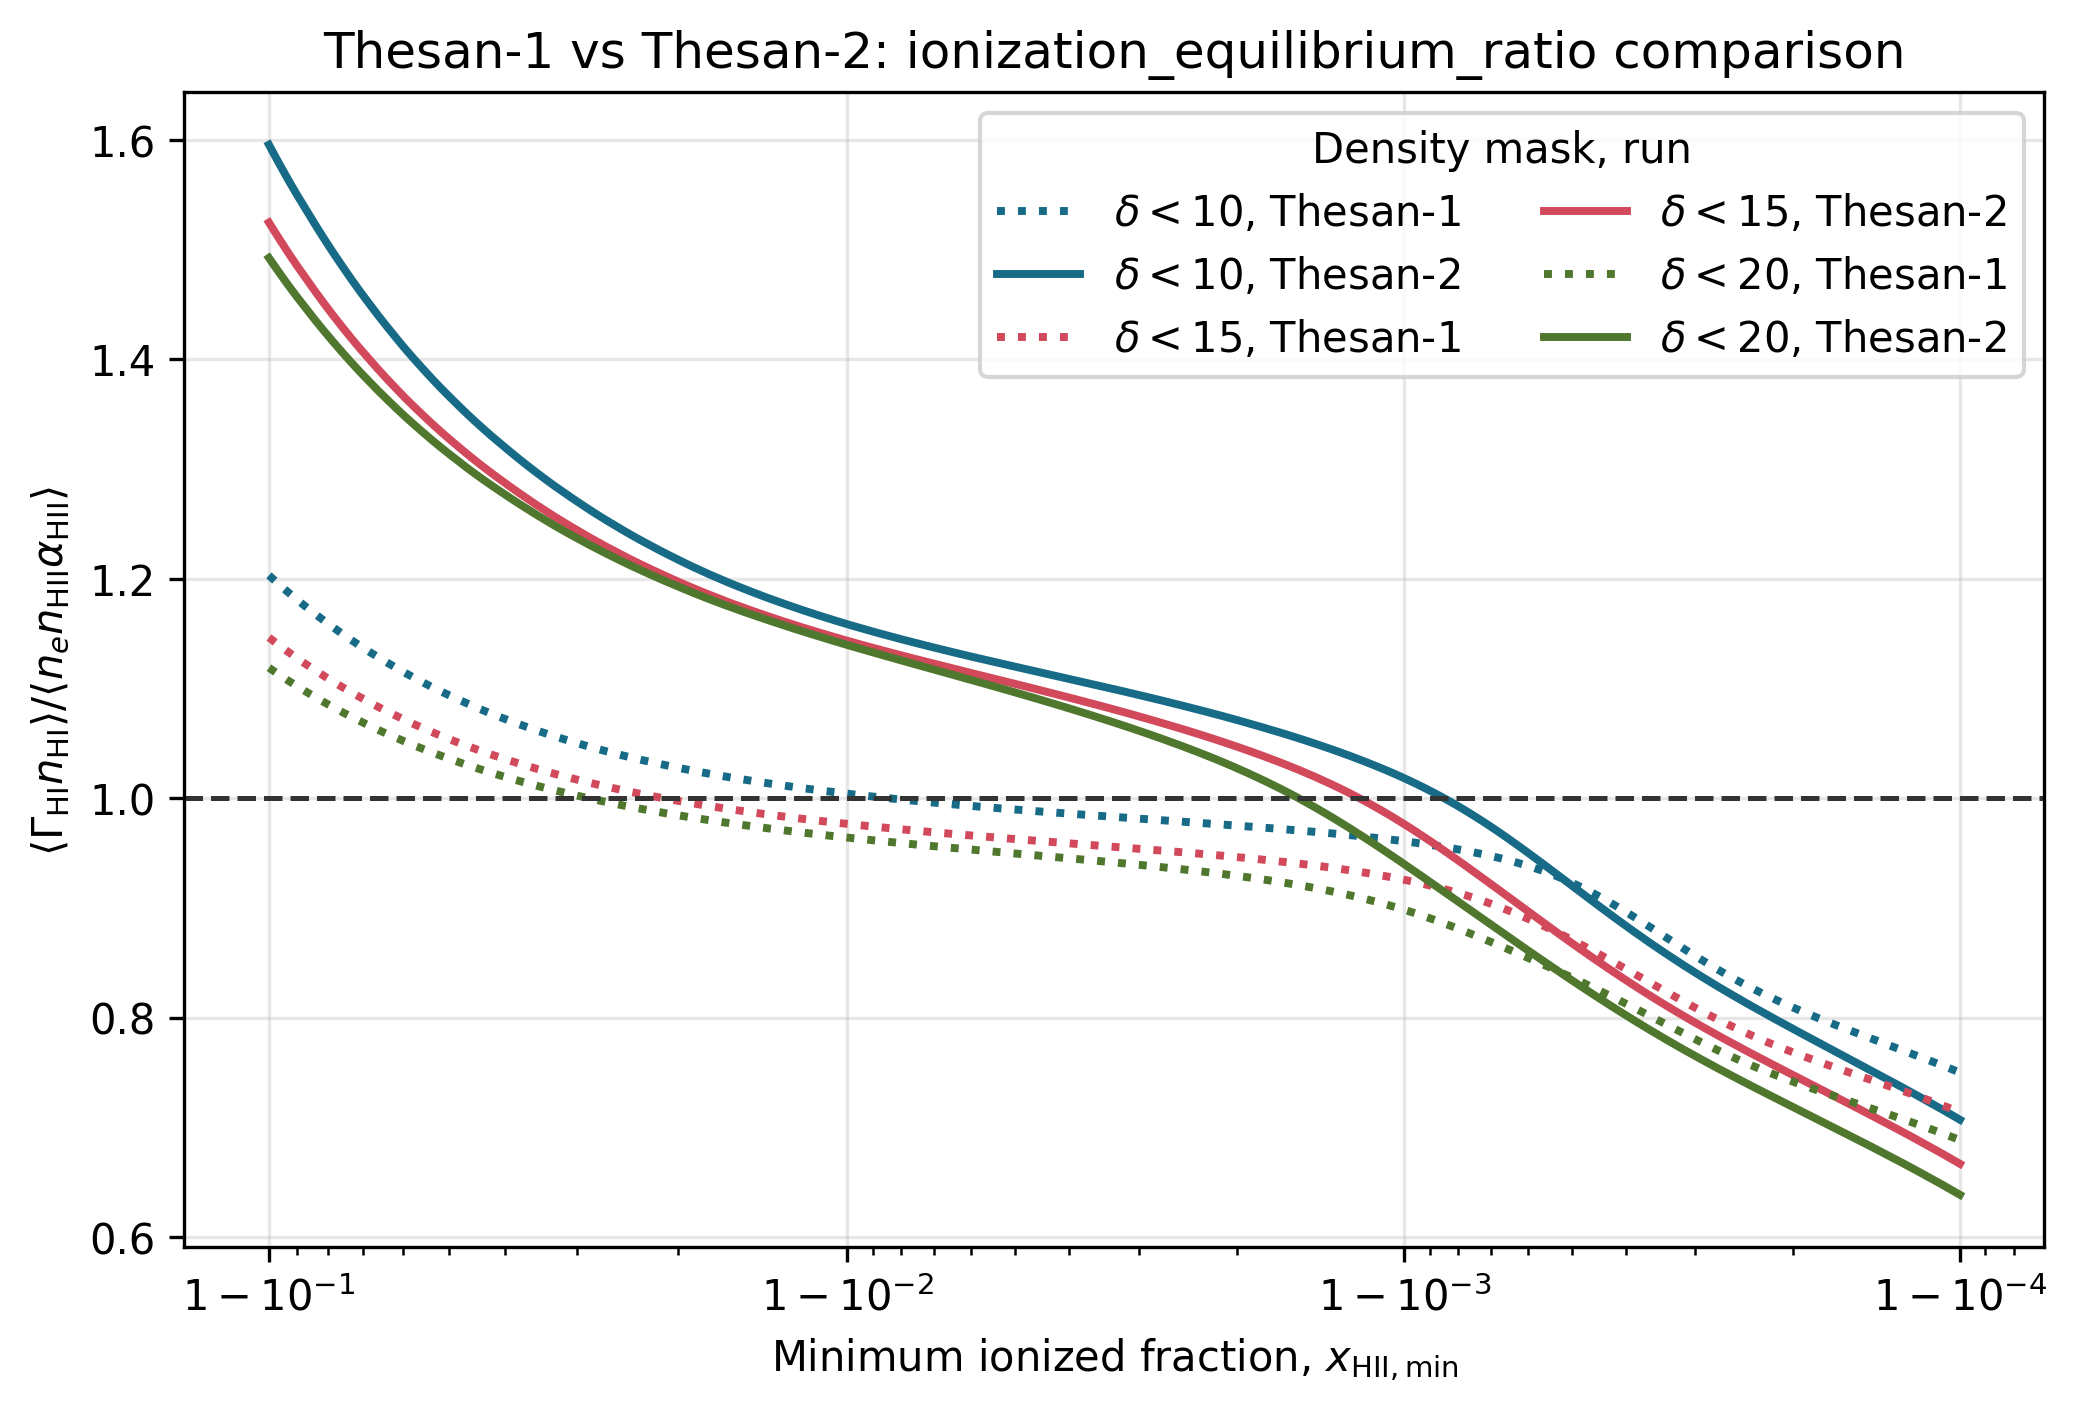
\includegraphics[width=\linewidth]{figures/thesan1_thesan2_ionization_equilibrium_ratio_vs_ionization_cut.png}
    \caption{Ratio of the photoionization and recombination rates as a function of the minimum ionized fraction used in the IGM mask. The horizontal line marks exact ionization equilibrium.}
    \label{fig:ionization-equilibrium}
\end{figure}

Davies et al. additionally approximate the mean free path by $\lambda_{\mathrm{mfp}}=(n_{\mathrm{H\,I}}\sigma_{\mathrm{H\,I}})^{-1}$. Figure~\ref{fig:meanfreepath-sigma} shows that this approximation introduces a systematic bias in the region where ionization equilibrium is closest to being satisfied. Thus, the two assumptions cannot generally be imposed simultaneously for the masks considered here.
\begin{figure}
    \centering
    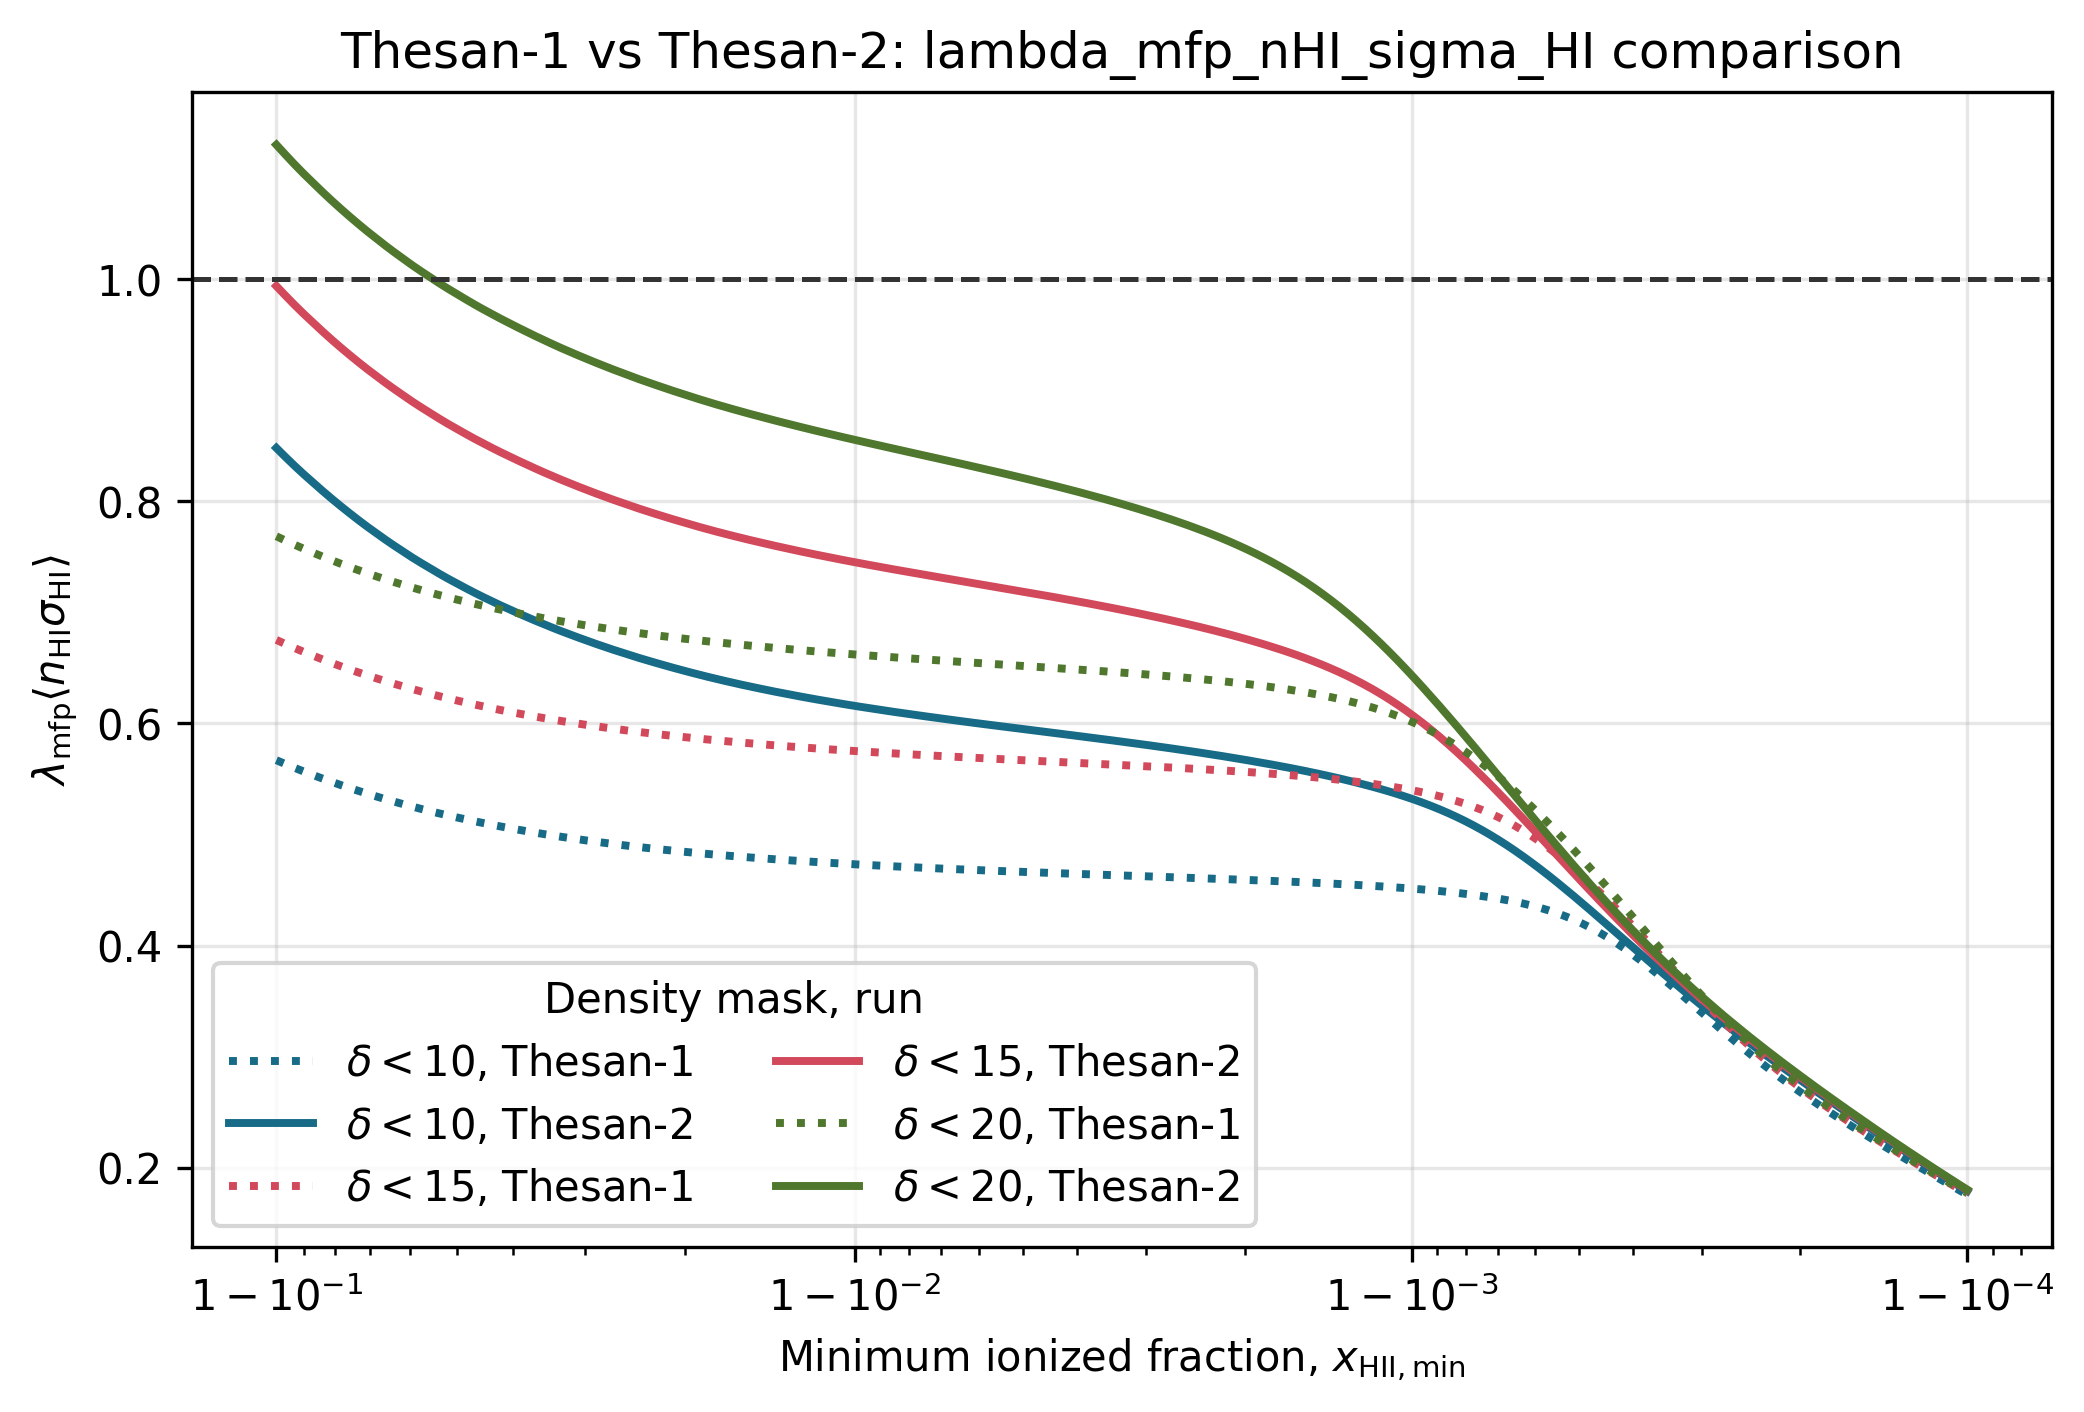
\includegraphics[width=\linewidth]{figures/thesan1_thesan2_lambda_mfp_nHI_sigma_HI_vs_ionization_cut.png}
    \caption{Ratio of the line-of-sight mean free path to the estimate $(n_{\mathrm{H\,I}}\sigma_{\mathrm{H\,I}})^{-1}$ as a function of the ionization cut. The horizontal line marks equality.}
    \label{fig:meanfreepath-sigma}
\end{figure}


Combining these assumptions gives the first approximate estimator,

$$C = \frac{ \Gamma_{\mathrm{H\,I}}}
{\lambda_{\mathrm{mfp}} \sigma_{\mathrm{H\,I}} \chi_e \left(1-x_{\mathrm{H\,I}}\right)^2 n_{\mathrm{H}}^2 \alpha_{\mathrm{H\,II}}}$$



\subsection{Approximate estimator 2: photon-density closure}
A second estimator defines an effective photon interaction rate by $\Gamma_{\gamma}=c/\lambda_{\mathrm{mfp}}$. The corresponding photoionization rate per unit volume is then assumed to balance the recombination rate:
$$\frac{n_{\gamma} c}{\lambda_{\mathrm{mfp}}}  = \langle n_e n_{\mathrm{H\,II}} \alpha_{\mathrm{H\,II}} \rangle .$$

The THESAN simulations use a reduced speed of light. We therefore use
the corresponding reduced value of $c$ in this relation. Even
after this correction, the relation is not satisfied for the masks
examined here. The resulting discrepancy is shown in
Fig.~\ref{fig:photon-density} and introduces an additional
multiplicative factor in the inferred clumping factor.

\begin{figure}
    \centering
    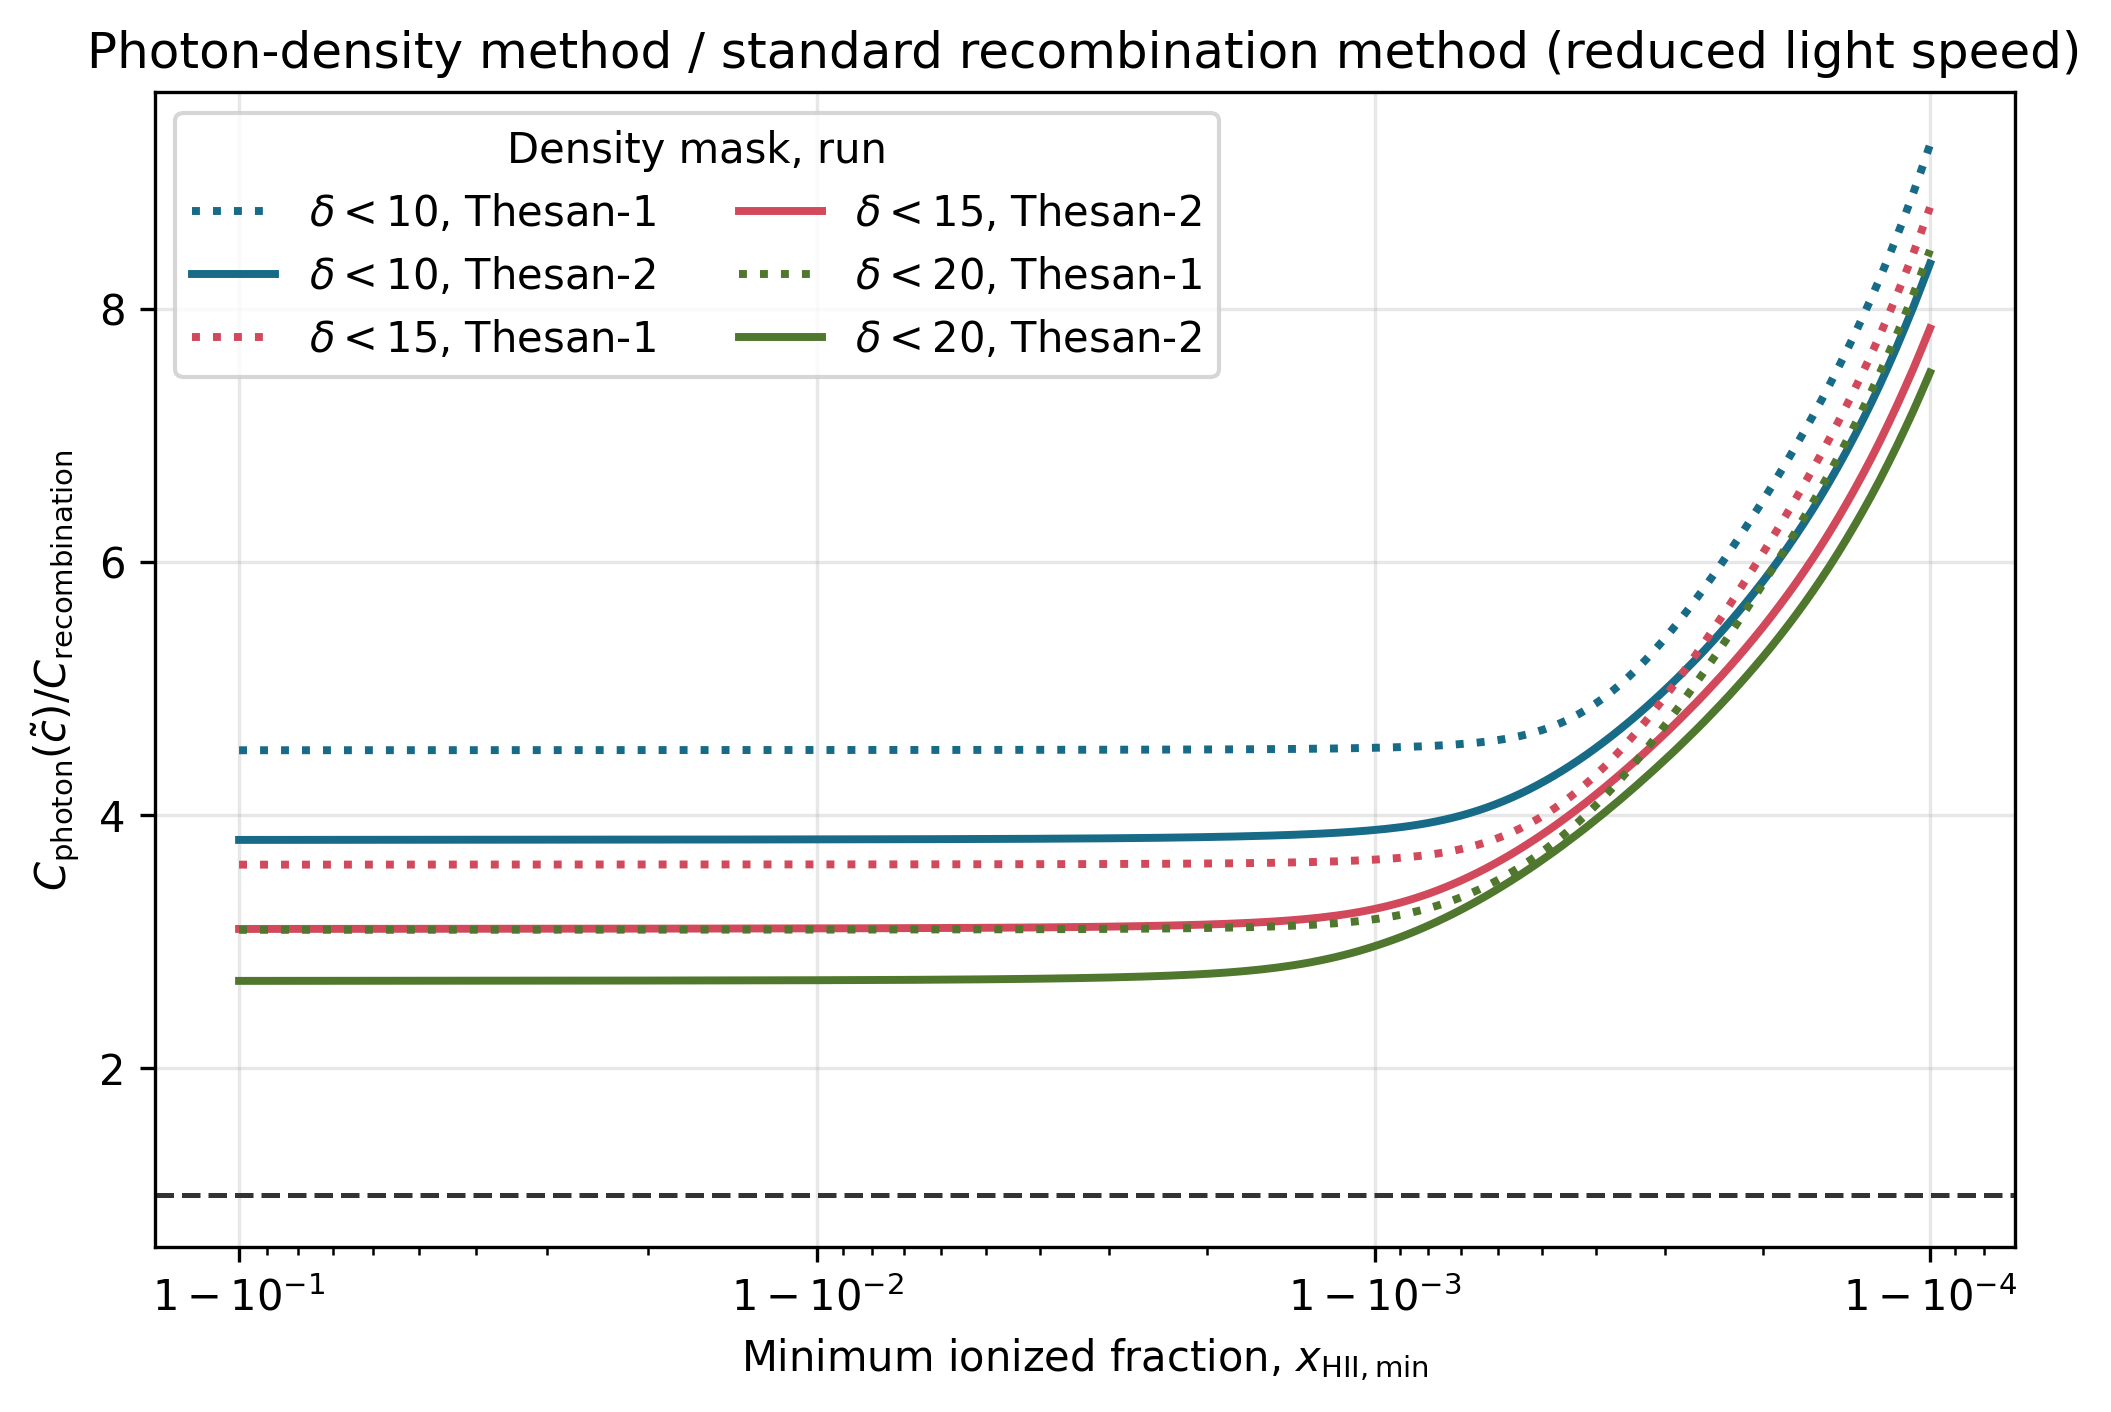
\includegraphics[width=\linewidth]{figures/thesan1_thesan2_photon_density_reduced_c_over_standard_vs_ionization_cut.png}
    \caption{Ratio between the photon-density estimate and the
    standard recombination rate, including the reduced speed of light,
    as a function of the minimum ionized fraction defining the IGM
    mask. The horizontal line marks agreement between the two rates.}
    \label{fig:photon-density}
\end{figure}

The resulting estimator is
$$C = \frac{ n_{\gamma} c}
{\lambda_{\mathrm{mfp}}  \chi_e \left(1-x_{\mathrm{H\,I}}\right)^2 n_{\mathrm{H}}^2 \alpha_{\mathrm{H\,II}}}.$$

\subsection{Comparison of clumping-factor estimators}

We have tested the assumptions entering the approximate estimators
individually. We now compare the resulting clumping factors with the
direct calculation for the THESAN simulations. The comparison is shown
in Fig.~\ref{fig:clumpingfactors} for several choices of the minimum
ionized fraction defining the IGM mask.

The direct calculation provides the reference result. Depending on the
overdensity threshold, its clumping factor is typically between
approximately 2 and 4. The estimator based on ionization equilibrium
gives a slightly larger value, with its closest agreement with the
reference result occurring for
$10^{-3}\lesssim x_{\mathrm{H\,II,min}}\lesssim10^{-2}$.

Including the additional approximation
$\lambda_{\mathrm{mfp}}=(n_{\mathrm{H\,I}}\sigma_{\mathrm{H\,I}})^{-1}$
increases the discrepancy. In the range where ionization equilibrium is
approximately satisfied, this estimator introduces a correction of up
to a factor of approximately 2.5 relative to the direct calculation.

The photon-density estimator gives the largest clumping factors. After
accounting for the reduced speed of light used in the THESAN
simulations, it still exceeds the direct estimate by up to a factor of
approximately 5 for the masks considered here.

\begin{figure*}[t]
    \centering
    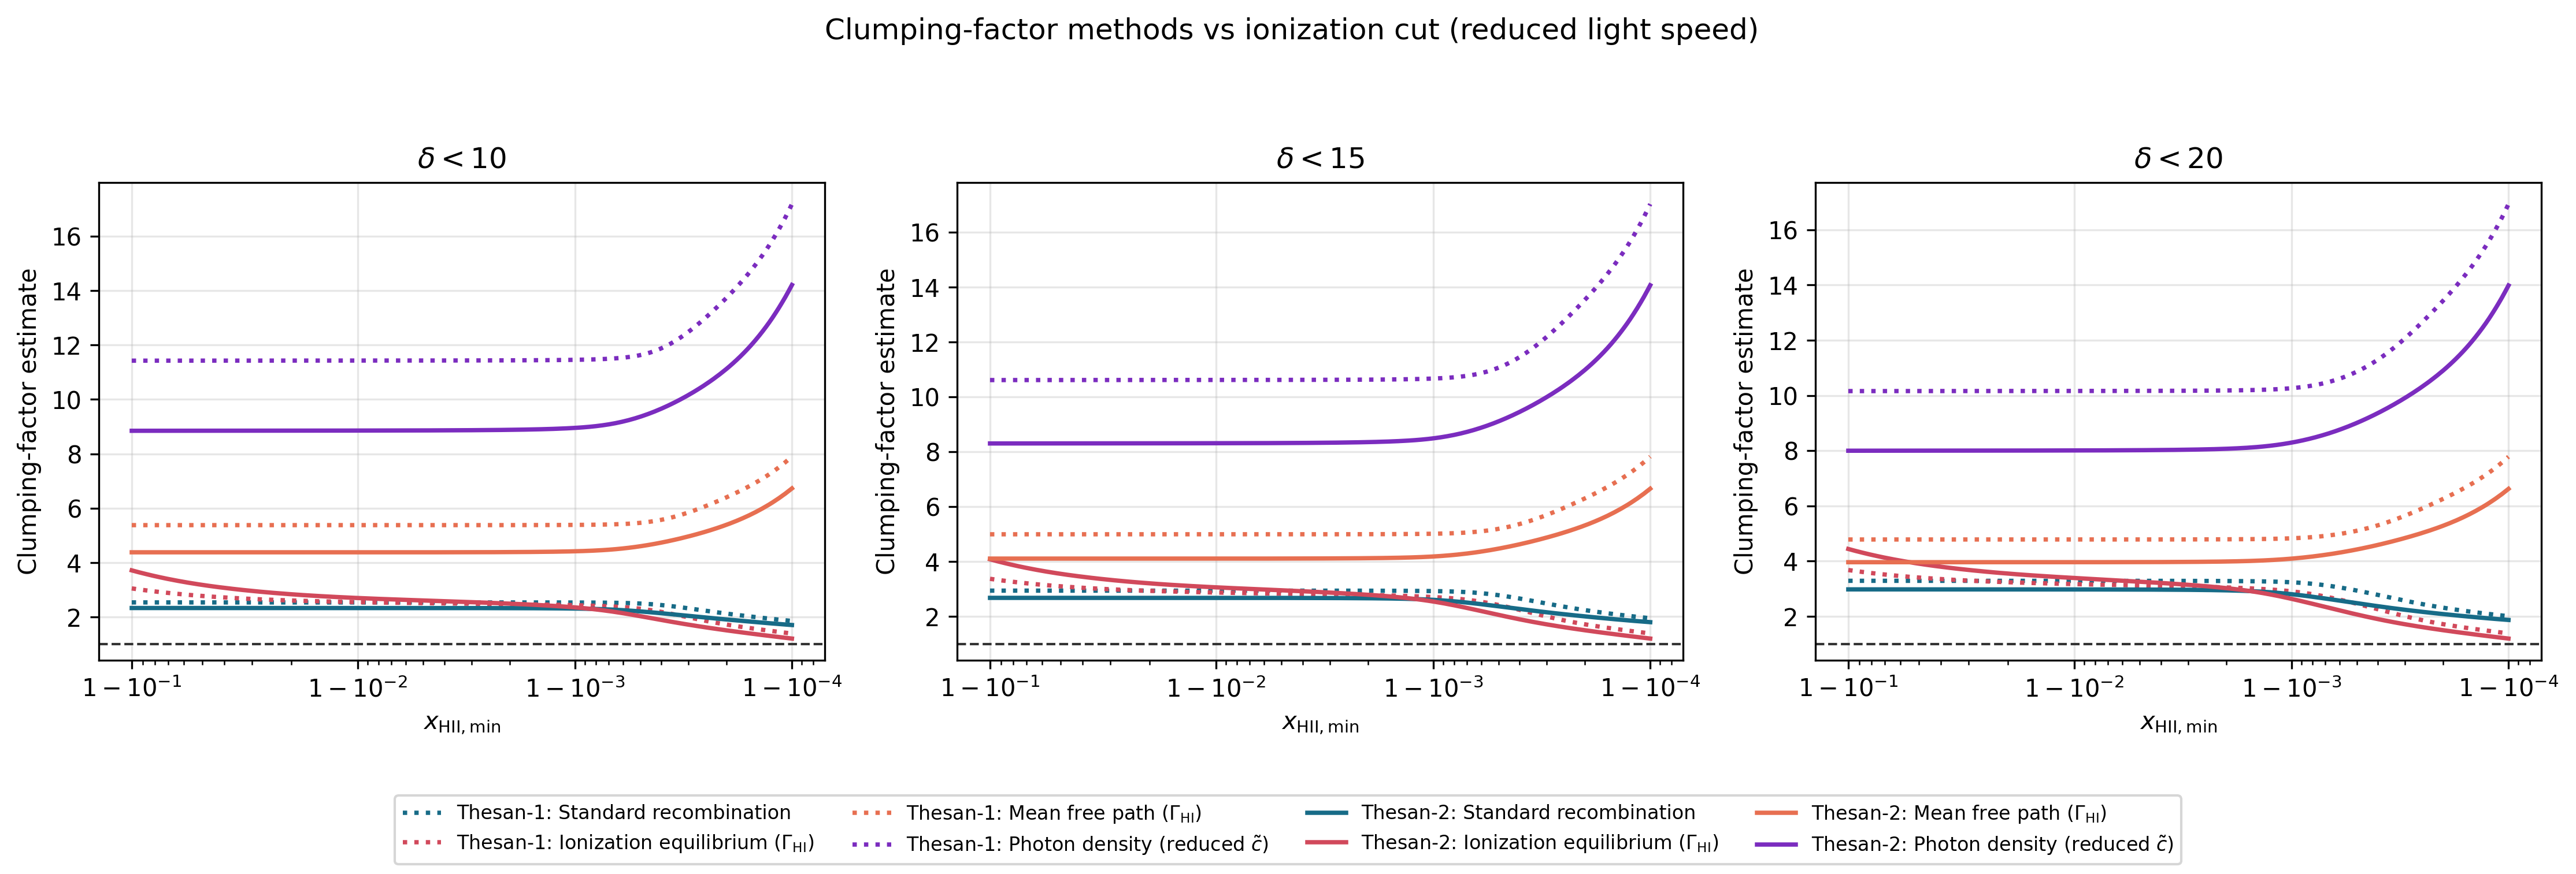
\includegraphics[width=0.96\textwidth]{figures/thesan1_thesan2_clumping_methods_reduced_c_vs_ionization_cut.png}
    \caption{Comparison of the direct and approximate clumping-factor
    estimators as a function of the minimum ionized fraction defining
    the IGM mask. The three panels correspond to overdensity thresholds
    $\Delta<10$, $\Delta<15$, and $\Delta<20$, respectively. The direct
    estimate is compared with the ionization-equilibrium, mean-free-path,
    and photon-density estimators. The photon-density estimator uses the
    reduced speed of light adopted in the THESAN simulations.}
    \label{fig:clumpingfactors}
\end{figure*}


\bibliography{apssamp}






Check in the appendix a comparison of the effects of the reduced speed of light


\section{Application II: Comparison between dark matter models}

\section{Power spectrum}
Reference the aida tng paper and the explanations they make

\section{Clumping factor}
Show calculations at different redshifts and the difference

Say we havent' found anything relevant at the current scales we can measure. 





\section{Disclosure of the use of AI in this work}
What things i've used AI in:
- This section
- Editorial review for mistakes
- Coding support, particularly for bug finding and familiarizing with large code infrastructures that have lots of documention (i.e. arepo) and with more technical tasks such as parallelization of current code
- Coding support for plot creation based on the existing results




\appendix
\section{Gridding impact in the AIDA-TNG simulations}

\label{apx:AIDA-TNG}

In this section, we validate the conclusions of Section~\ref{sec:density-grid-tests} in the context of the AIDA-TNG simulations. As described in Section~III.A, the matter distribution is represented by dark-matter particles and finite-volume gas Voronoi cells. We therefore repeat the comparison between the direct Voronoi-cell calculation and a standardized mass-deposited grid before applying the adopted choices to the dark-matter fields. Furthermore, we introduce figures in which the SubfindHsml particle property is used to determine the smoothing scale and the clumping factor, rather than adopting the interparticle distance as a universal particle size.

\subsection{Grid-size tests and gridding deviation}

We first repeat the grid-size comparison using the gas fields of the AIDA-TNG simulations. Following the density-field construction described in Section~III.A, the gas cells are treated as point-like elements carrying their cell masses when constructing the standardized mass-deposited grid. We use cloud-in-cell as the mass-assignment scheme and apply top-hat smoothing to the resulting density field. To compare the gridded estimates with the direct Voronoi-cell result over the full overdensity range, we use the normalized gridding-deviation factor introduced in Section~\ref{sec:density-grid-tests},
\begin{equation}
    \Delta_{grid} = \int_{0}^{25}
    \frac{C_{Voronoi} - C_{grid}}
    {C_{Voronoi}}\,\mathrm{d}\delta,
    \label{eq:aida-gridding-deviation}
\end{equation}
where $C_{Voronoi}$ is the clumping factor calculated directly from the native Voronoi cells and $C_{grid}$ is the estimate obtained from the standardized mass-deposited grid. Positive values indicate that the gridded calculation underestimates the direct Voronoi-cell result over the integrated overdensity range, whereas negative values indicate an overestimate.

\begin{figure*}[t]
    \centering
    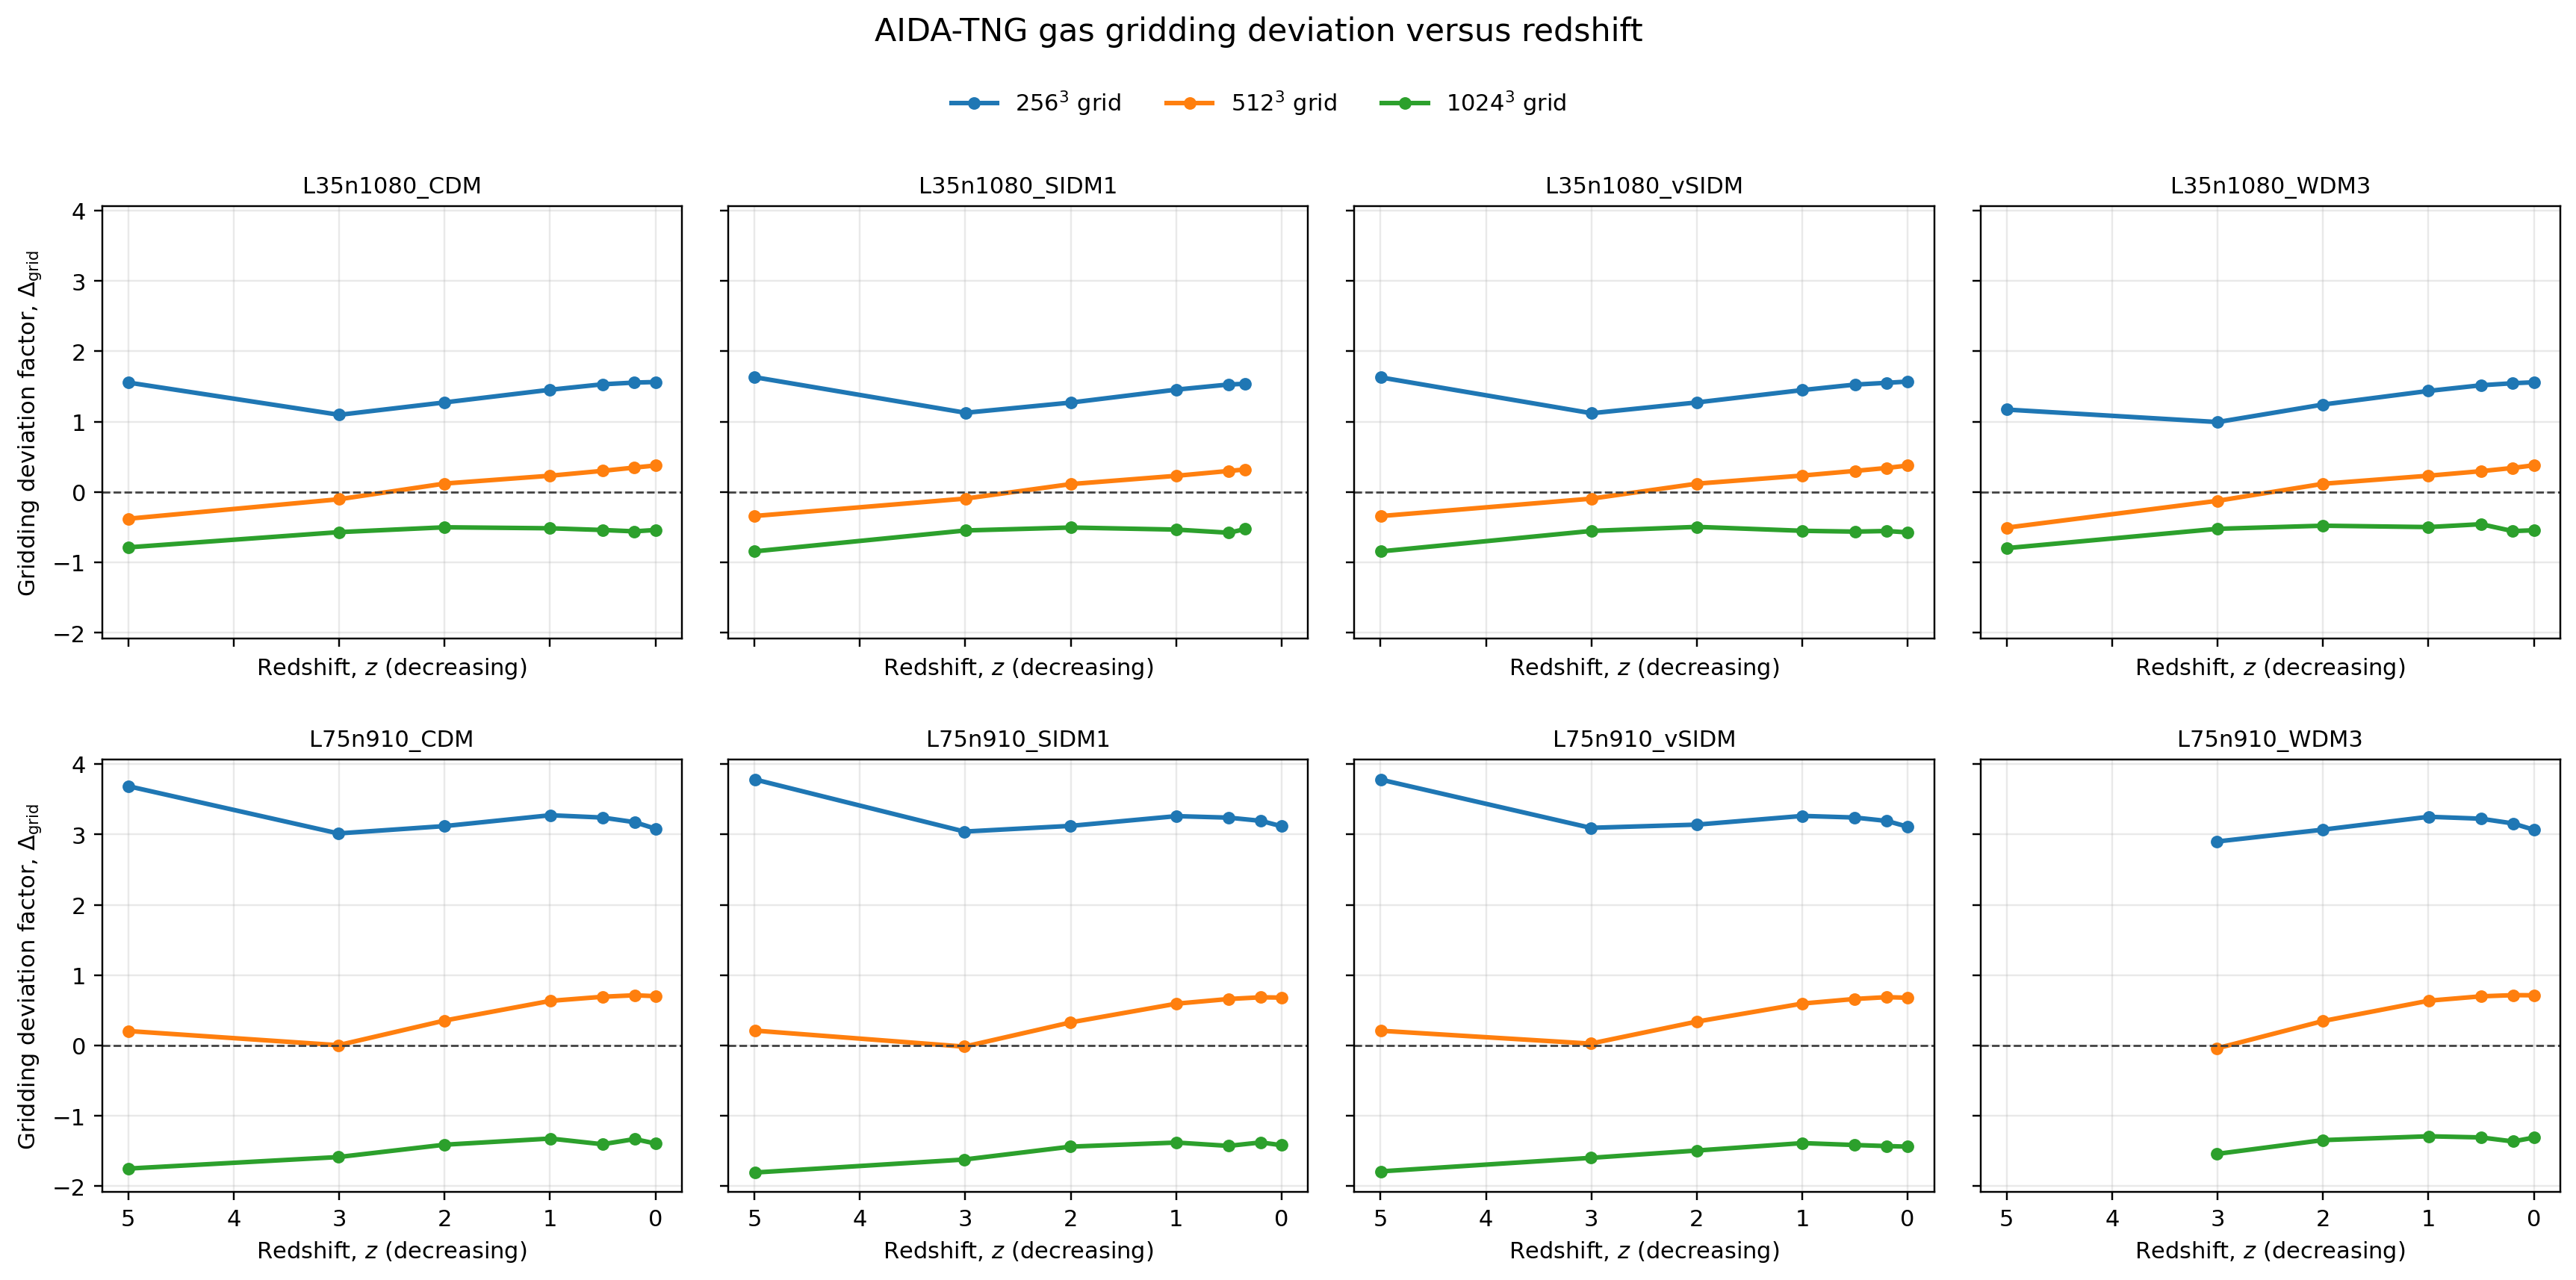
\includegraphics[width=\textwidth]{figures/aida_tng_grid_deviation_vs_redshift_no_formula.png}
    \caption{Normalized gridding-deviation factor, Eq.~\eqref{eq:aida-gridding-deviation}, for the gas fields of the AIDA-TNG simulations. Each panel corresponds to one dark-matter model and simulation box. The curves show estimates from standardized mass-deposited grids with cloud-in-cell mass assignment and top-hat smoothing at $256^3$, $512^3$, and $1024^3$ grid cells, using the direct Voronoi-cell calculation as the reference. The redshift axis decreases from left to right; only snapshots for which all three grid calculations and the direct Voronoi-cell result are available are shown.}
    \label{fig:aida-gridding-deviation-factor}
\end{figure*}

Figure~\ref{fig:aida-gridding-deviation-factor} shows that the qualitative ordering found for THESAN is also present in AIDA-TNG. The $256^3$ estimates remain below the direct Voronoi-cell result, while the $1024^3$ estimates generally lie above it. The $512^3$ grid gives the smallest integrated mismatch and is the closest of the three gridded estimates to the direct Voronoi-cell result across the available redshifts. The same ordering is observed for the different dark-matter models within a given box, indicating that the dominant effect is the density-field resolution rather than the particular dark-matter interaction model. The deviations are larger for the $75\,h^{-1}\,\mathrm{Mpc}$ box, whose lower particle sampling makes the grid-to-particle ratio less favorable. These results support the use of the intermediate gridding factor adopted for the AIDA-TNG dark-matter calculations.

\section{Impact of the Reduced Speed of Light on the THESAN Observables}
\label{apx:reduced-speed-of-light}

\subsection{Aim and scope}

The main text uses the reduced speed of light adopted in the THESAN
radiation-transport calculations when evaluating the photon-density
estimator. In this appendix, we document a pilot comparison between the
in-house simulations run with the standard speed of light and with the
reduced speed of light. We examine the direct recombination clumping factor,
the ionization-equilibrium estimator, the photon-density estimator, and the
mean-free-path closure.

The purpose of this comparison is diagnostic. The in-house standard-speed
and reduced-speed runs are useful as a paired test of the current
implementation, but the comparison is not by itself a fully controlled
convergence study. Differences between the available outputs can also be
affected by the simulation volume, resolution, initial conditions, source
history, snapshot selection, and the IGM mask. We therefore do not interpret
the comparison as a universal correction to the reduced speed of light.

\subsection{Simulation suite and comparison metadata}

Table~\ref{tab:reduced-speed-metadata} summarizes the outputs used in the
figures. The full THESAN runs are included as reference calculations for the
context of the main analysis. The paired in-house runs are the closest
standard-speed/reduced-speed comparison currently available.

\begin{table*}[t]
    \centering
    \caption{Simulation and analysis metadata for the reduced-speed-of-light
    comparison. The redshifts and snapshot identifiers are those recorded in
    the current structured equation-test results. The ``raw'' mask means that
    the figures use an overdensity threshold without an additional ionized
    fraction cut.}
    \label{tab:reduced-speed-metadata}
    \resizebox{\textwidth}{!}{\normalsize%
    \begin{tabular}{llllll}
        \hline
        Run & Snapshot & Redshift & Light-speed prescription & Particle setup & Figure selection \\
        \hline
        THESAN-1 & 080 & 5.512 & THESAN reduced-speed prescription & full THESAN & raw $\Delta$ masks \\
        THESAN-2 & 080 & 5.491 & THESAN reduced-speed prescription & full THESAN & raw $\Delta$ masks \\
        mini SL & 015 & 4.000 & standard $c$ & $4\,\mathrm{Mpc}$, $128^3$ & raw $\Delta$ masks \\
        mini RSL & 015 & 4.000 & reduced $\tilde{c}$ & $4\,\mathrm{Mpc}$, $128^3$ & raw $\Delta$ masks \\
        \hline
    \end{tabular}}
\end{table*}

The current mini-SL result does not contain the same ionized-fraction sweep
as the mini-RSL result. For this reason, Figures~\ref{fig:sl-rsl-absolute}
and~\ref{fig:sl-rsl-ratio} use only the common raw overdensity masks. This
keeps the plotted selections explicit and avoids mixing an ionization-cut
measurement with a raw overdensity measurement. The provenance metadata for
the mini-SL result should also be checked before the numerical comparison is
treated as final, since its recorded base path currently references the
$4\times128^3$ reduced-speed output directory.

\subsection{Definitions and comparison protocol}

The direct reference quantity is the recombination-weighted clumping factor
$C_{\rm rec}$ defined in the main text. We also show the ionization-equilibrium
quantity $C_7$ and the photon-density quantity $C_{13,\tilde c}$ as they are
recorded by the current analysis pipeline. The mean-free-path quantity,

\begin{equation}
    R_{\rm mfp} =
    \frac{\langle n_{\rm HI}\rangle_{\lambda}}
    {\langle n_{\rm HI}\rangle_V},
\end{equation}

is a closure ratio rather than an independent clumping-factor definition.
Equality of the two mean neutral-hydrogen estimates corresponds to
$R_{\rm mfp}=1$.

The comparison uses the nearest available raw overdensity rows to
$\Delta_{\rm max}=10$, $15$, and $20$. For the paired in-house comparison,
we show both the absolute values and the ratio of the reduced-speed result
to the standard-speed result,

\begin{equation}
    R_{\rm RSL/SL}(X) = \frac{X_{\rm mini\,RSL}}
    {X_{\rm mini\,SL}}.
\end{equation}

The ratio is a diagnostic of the current paired outputs. It is not interpreted
as a causal measurement of the speed-of-light effect without additional
matched simulations.

\subsection{In-house standard-speed and reduced-speed comparison}

Figure~\ref{fig:sl-rsl-absolute} shows the four quantities for the two
in-house runs. The direct recombination result and the radiation-dependent
estimators are shown together so that changes in the underlying clumping
quantity can be distinguished from changes in the closure relations.

\begin{figure*}[t]
    \centering
    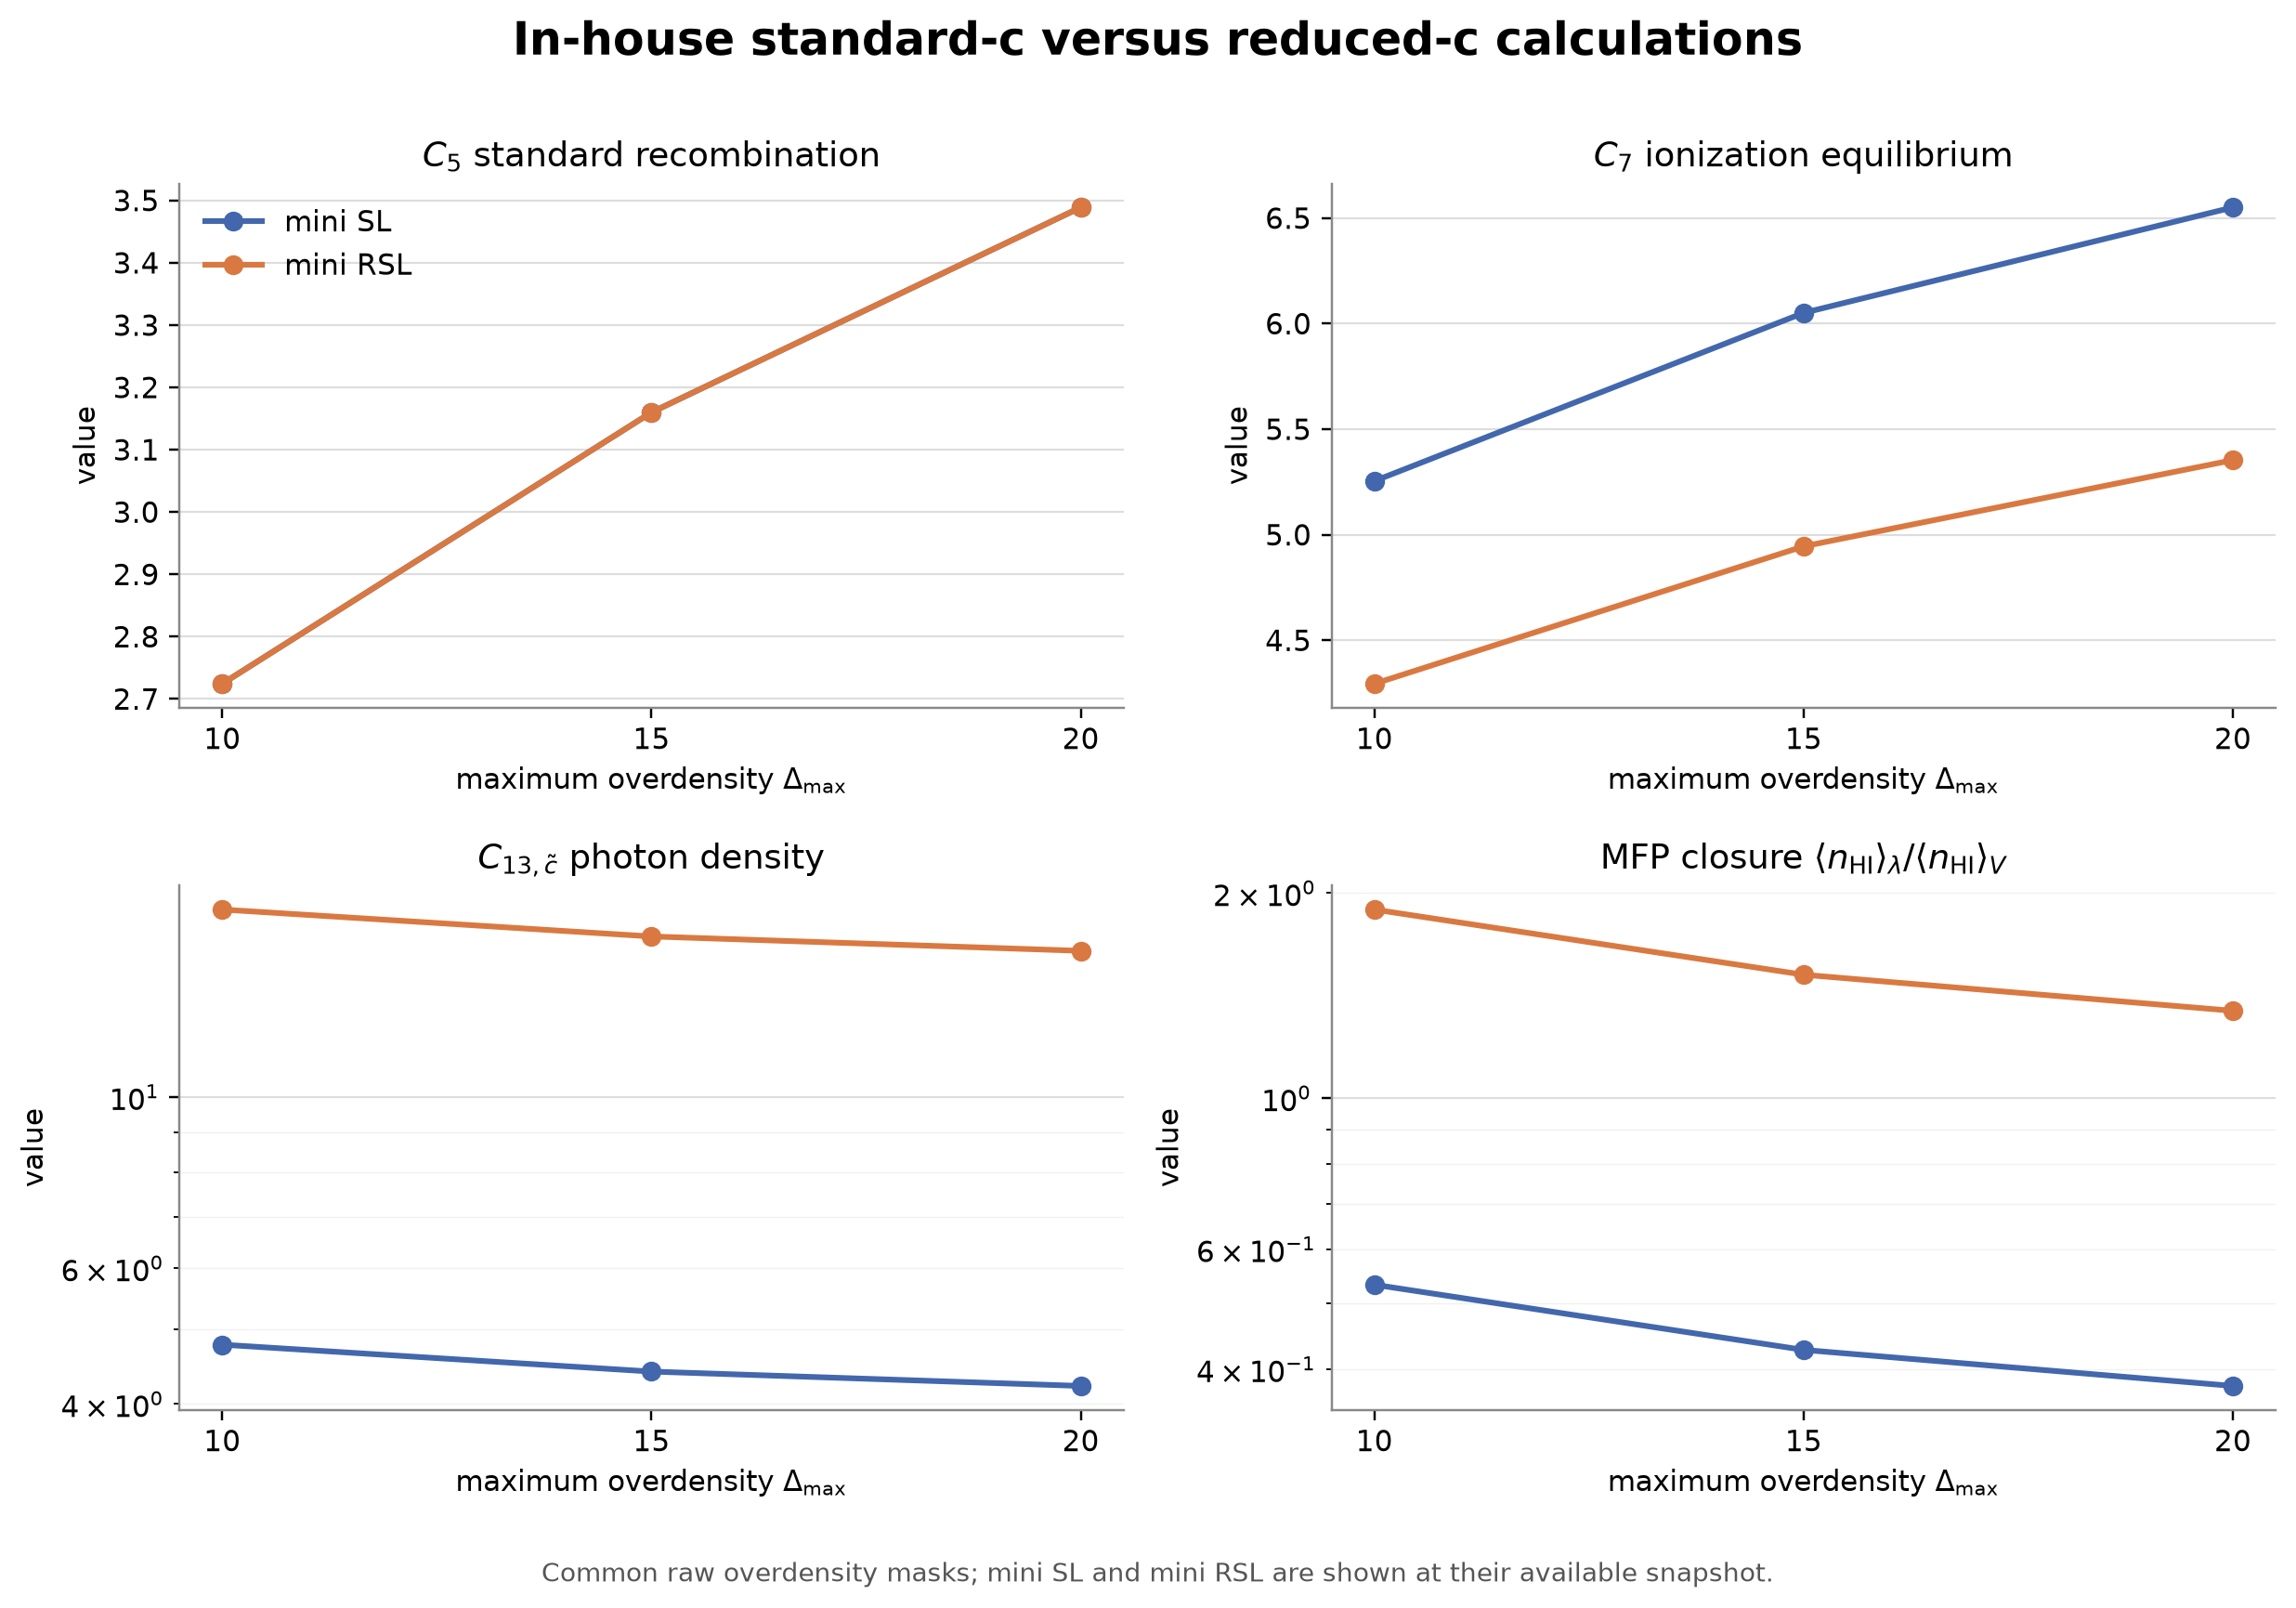
\includegraphics[width=0.96\textwidth]{figures/thesan_speed_of_light_inhouse_absolute.png}
    \caption{Absolute comparison of the in-house standard-speed (mini SL) and
    reduced-speed (mini RSL) outputs. Each panel uses the common raw
    overdensity masks at the available snapshot. The photon-density and
    mean-free-path panels use logarithmic vertical axes.}
    \label{fig:sl-rsl-absolute}
\end{figure*}

Figure~\ref{fig:sl-rsl-ratio} presents the same comparison as the ratio of the
reduced-speed result to the standard-speed result. The horizontal line marks
equality. These ratios show where the paired outputs differ, but they do not
separate the speed-of-light prescription from any remaining differences in
the simulation metadata or radiation history.

\begin{figure*}[t]
    \centering
    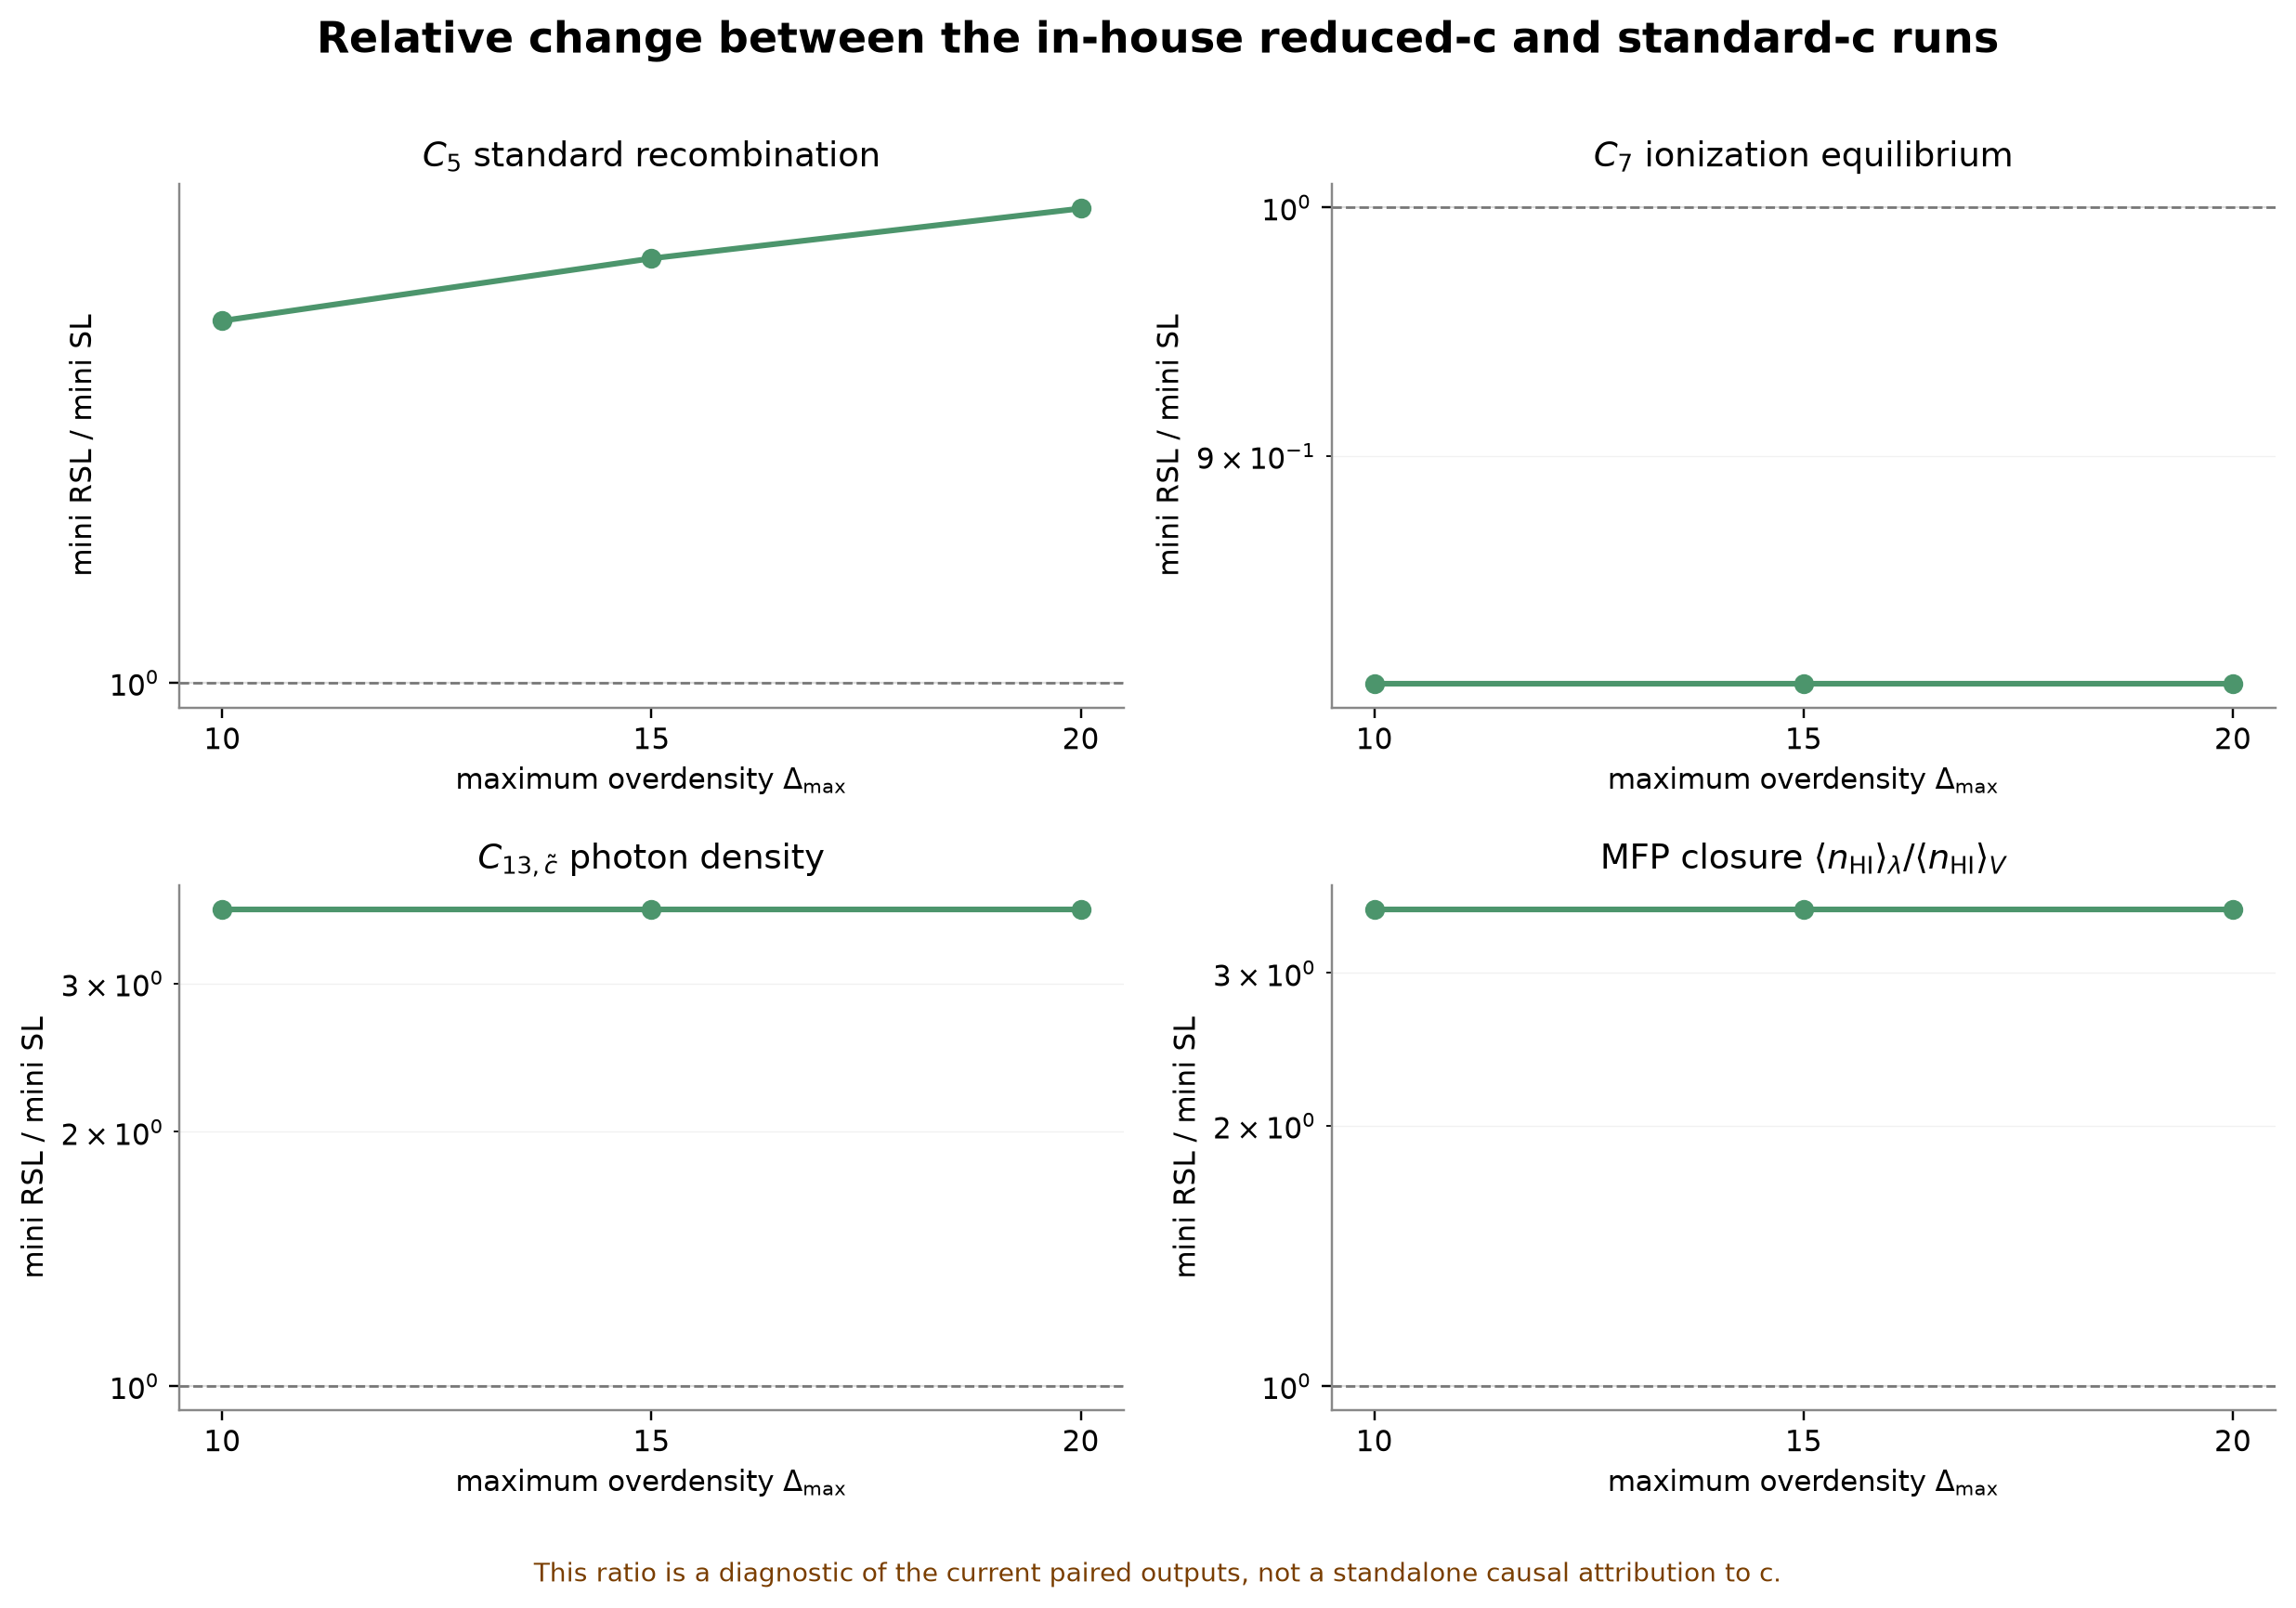
\includegraphics[width=0.96\textwidth]{figures/thesan_speed_of_light_inhouse_ratio.png}
    \caption{Ratio of the mini-RSL to mini-SL results for the same four
    observables. The dashed line marks equality. This figure is a diagnostic
    comparison of the available paired outputs and is not a standalone causal
    attribution to the speed of light.}
    \label{fig:sl-rsl-ratio}
\end{figure*}

\subsection{Context from the full THESAN runs}

Figure~\ref{fig:full-thesan-speed-comparison} places the in-house outputs
alongside THESAN-1 and THESAN-2 at the same nominal overdensity thresholds.
The comparison is intended to show the range of values represented by the
available calculations and to connect the pilot runs with the full THESAN
results used in Section~\ref{sec:appl1}. It should not be read as a matched
full-volume speed-of-light experiment: the full and in-house calculations
are at different redshifts and do not provide identical volume, resolution,
initial-condition, or source-history controls.

\begin{figure*}[t]
    \centering
    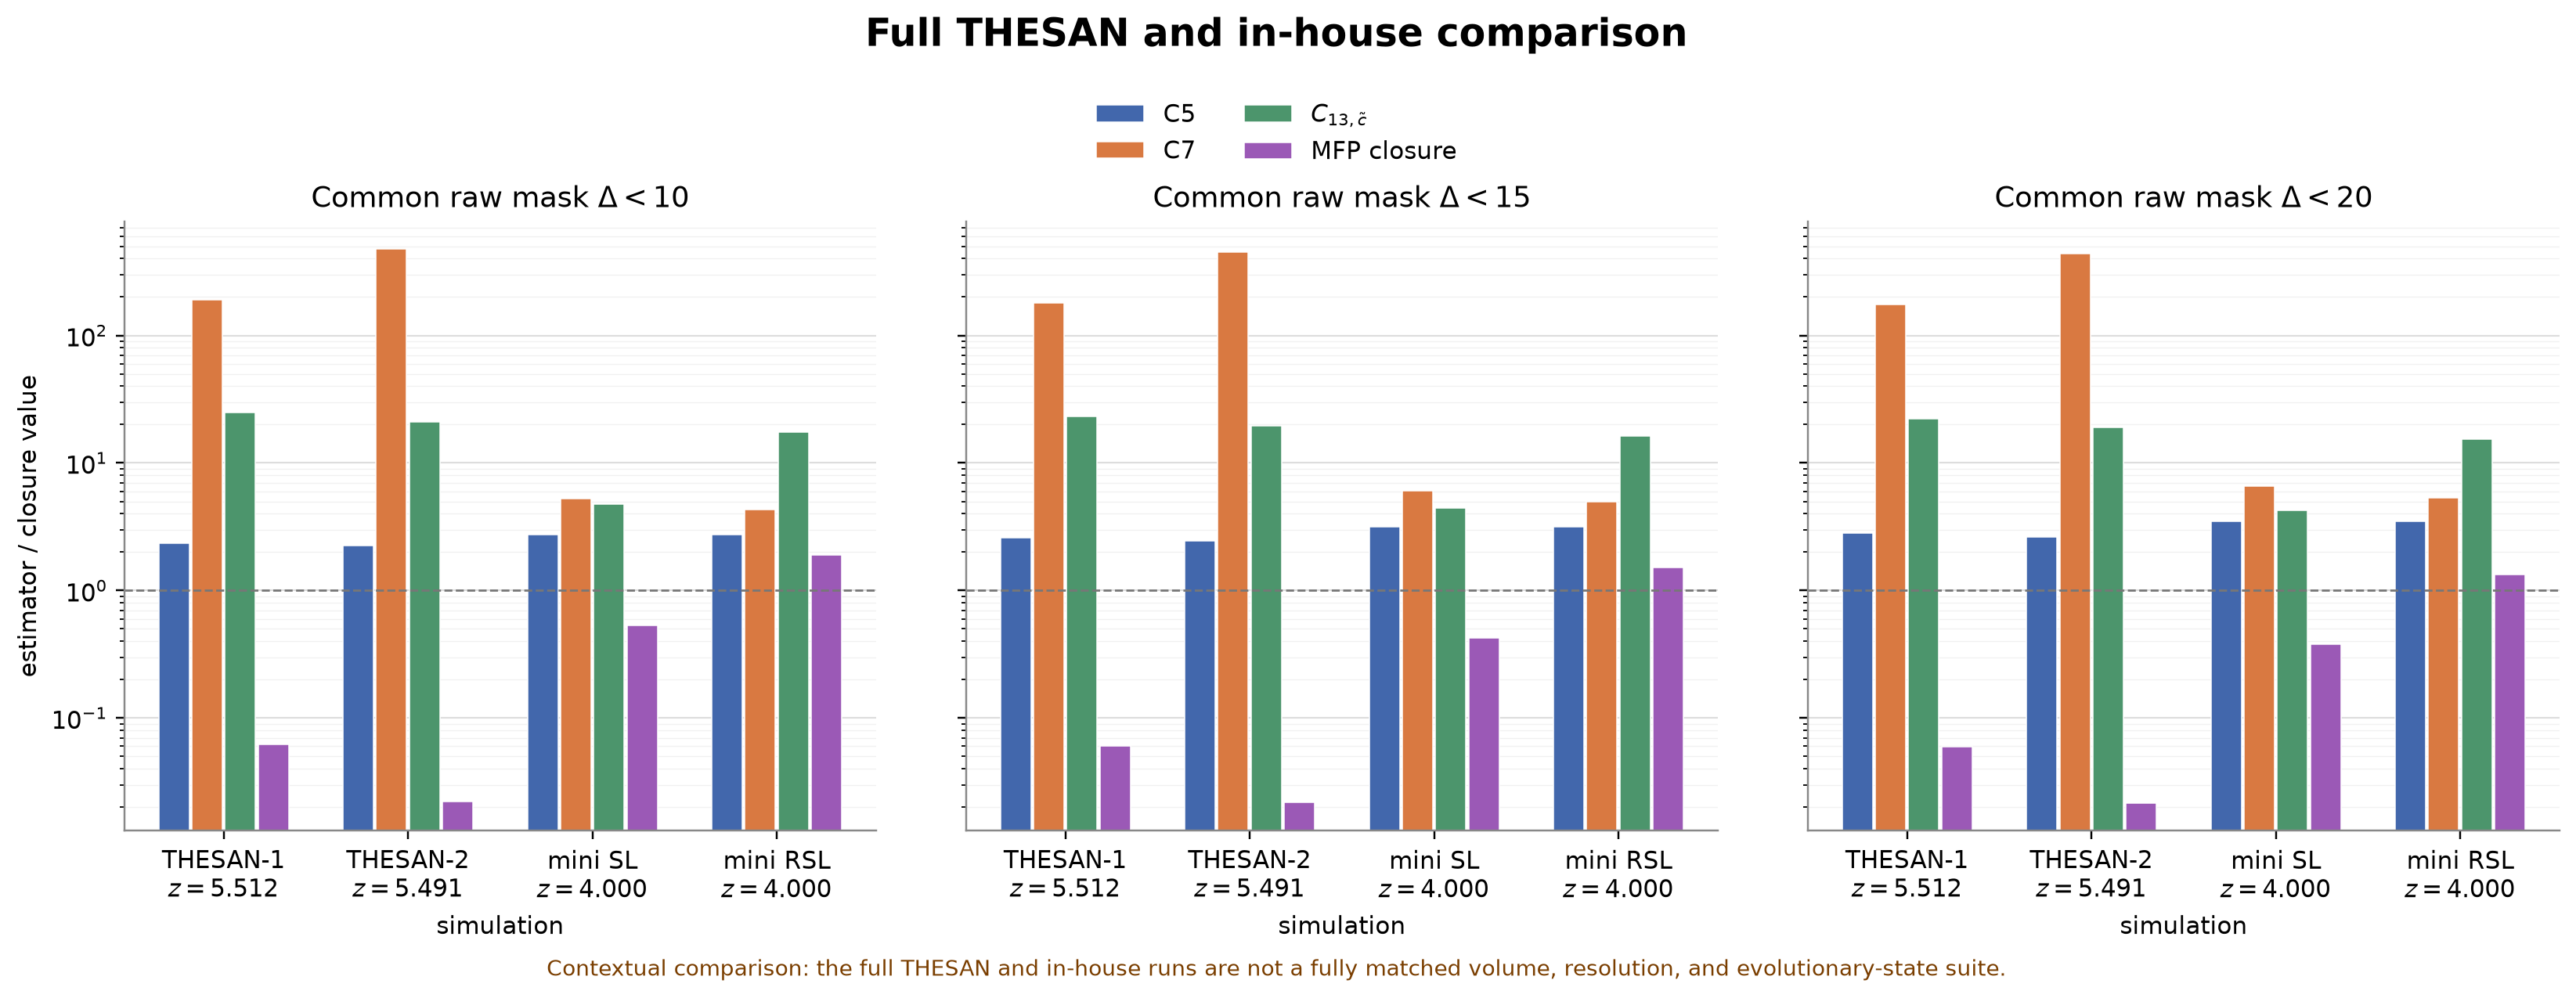
\includegraphics[width=0.98\textwidth]{figures/thesan_speed_of_light_full_comparison.png}
    \caption{Contextual comparison of the full THESAN and in-house outputs at
    common raw overdensity masks. The three panels show $\Delta<10$,
    $\Delta<15$, and $\Delta<20$. The direct recombination quantity, the
    ionization-equilibrium quantity, the reduced-speed photon-density
    quantity, and the mean-free-path closure are shown on a logarithmic scale.
    The full THESAN and in-house runs are not a fully matched volume,
    resolution, and evolutionary-state suite.}
    \label{fig:full-thesan-speed-comparison}
\end{figure*}

\subsection{Interpretation limits and planned larger simulations}

The figures above document the current pilot comparison but do not establish
a universal speed-of-light correction, volume-converged behavior, or the
behavior of the estimators at other redshifts and source histories. In
particular, the comparison does not demonstrate that every difference
between the full THESAN and in-house results is caused by the radiation
propagation speed. The existing conclusions in Section~\ref{sec:appl1}
about the separate estimator assumptions therefore remain the scope of the
present analysis.

A further comparison is planned using simulations with double the size of
the present in-house setup, together with an extended version of the
comparison shown here. These calculations are intended to test whether the
behavior seen in the pilot runs persists when the sampled volume and
available structure are increased. They could not be completed within the
time available for this report and are not included in the present results.
No conclusion is drawn here about how the larger simulations will modify the
patterns shown above.

\section{Parallelization and optimization: Working with large simulations}
\label{apx:parallelization}

The density-grid calculations are the most memory-intensive part of the
clumping-factor pipeline.  A direct calculation requires the particle data,
the density grid, and the intermediate arrays used by the smoothing and
threshold operations to coexist in memory.  The implementation therefore
uses a chunked execution path whenever the estimated full-load size exceeds
the configured limit.  The chunked path preserves the scientific operation
while changing how the input is scheduled and how temporary grids are
combined.

\subsection{Work decomposition and reduction}

The HDF5 snapshot is read as a stream of bounded particle chunks.  A parent
process first inspects the snapshot metadata and creates a deterministic work
plan.  The default plan assigns complete snapshot files to workers using a
greedy load-balancing rule.  When the file sizes are sufficiently imbalanced,
the plan subdivides large files into particle ranges.  This avoids assuming
that the number of files is an adequate proxy for the amount of work while
still limiting the number of independent readers per file.

Each process owns a private density-grid accumulator.  Workers read their
assigned chunks, apply the same mass-assignment and smoothing operations as
the serial path, and write their private grids to temporary NumPy files.
The parent process reduces these files into the final grid and removes each
temporary file after it has been incorporated.  Consequently, workers never
write concurrently to a shared grid, and the reduction order does not change
the physical input data or the definition of the clumping factor.  The same
private-grid and reduction pattern is used by the SciPy and Pylians chunked
grid builders.

\subsection{Memory policy and diagnostics}

Parallelism is constrained by the memory required for the private grids.  If
$B_g$ is the size of one grid, $w$ is the effective worker count, and $b$ is
the number of radius bins processed per stream pass, the implementation
estimates the grid-related allocation as
\begin{equation}
    B_{\mathrm{grid}} \simeq B_g\left[1+w(b+2)\right].
    \label{eq:parallel-grid-memory}
\end{equation}
The configured safety fraction reserves space for Python, HDF5, and other
non-grid allocations.  When the estimate exceeds the memory limit, the
policy reduces the worker count first and then the radius-bin batch size.  If
even one worker with one radius-bin batch cannot fit, the calculation fails
before starting the worker pool.  Result metadata records the requested and
effective worker counts, partition mode, private-grid estimates, worker
assignment, I/O, preprocessing, smoothing, and reduction times.

\subsection{Existing validation evidence}

The parallel path is validated at two levels.  First, the chunked-loading
test suite contains 21 tests covering serial--parallel equality for the cube
and Pylians paths, deterministic file and range partitioning, automatic
range selection, memory-policy reductions, cache invalidation, temporary
file cleanup, and worker-failure cleanup.  These tests pass without changing
the numerical tolerances used by the production calculations.

Second, the existing Thesan-2 worker overlays show that the clumping-factor
curves and selected-cell counts remain coincident as the worker count changes.
The overlays are reproduced from the existing analysis artifacts in
Fig.~\ref{fig:parallel-worker-clumping} and Fig.~\ref{fig:parallel-worker-cells};
they are numerical-parity diagnostics, not new simulations.

\begin{figure}[t]
    \centering
    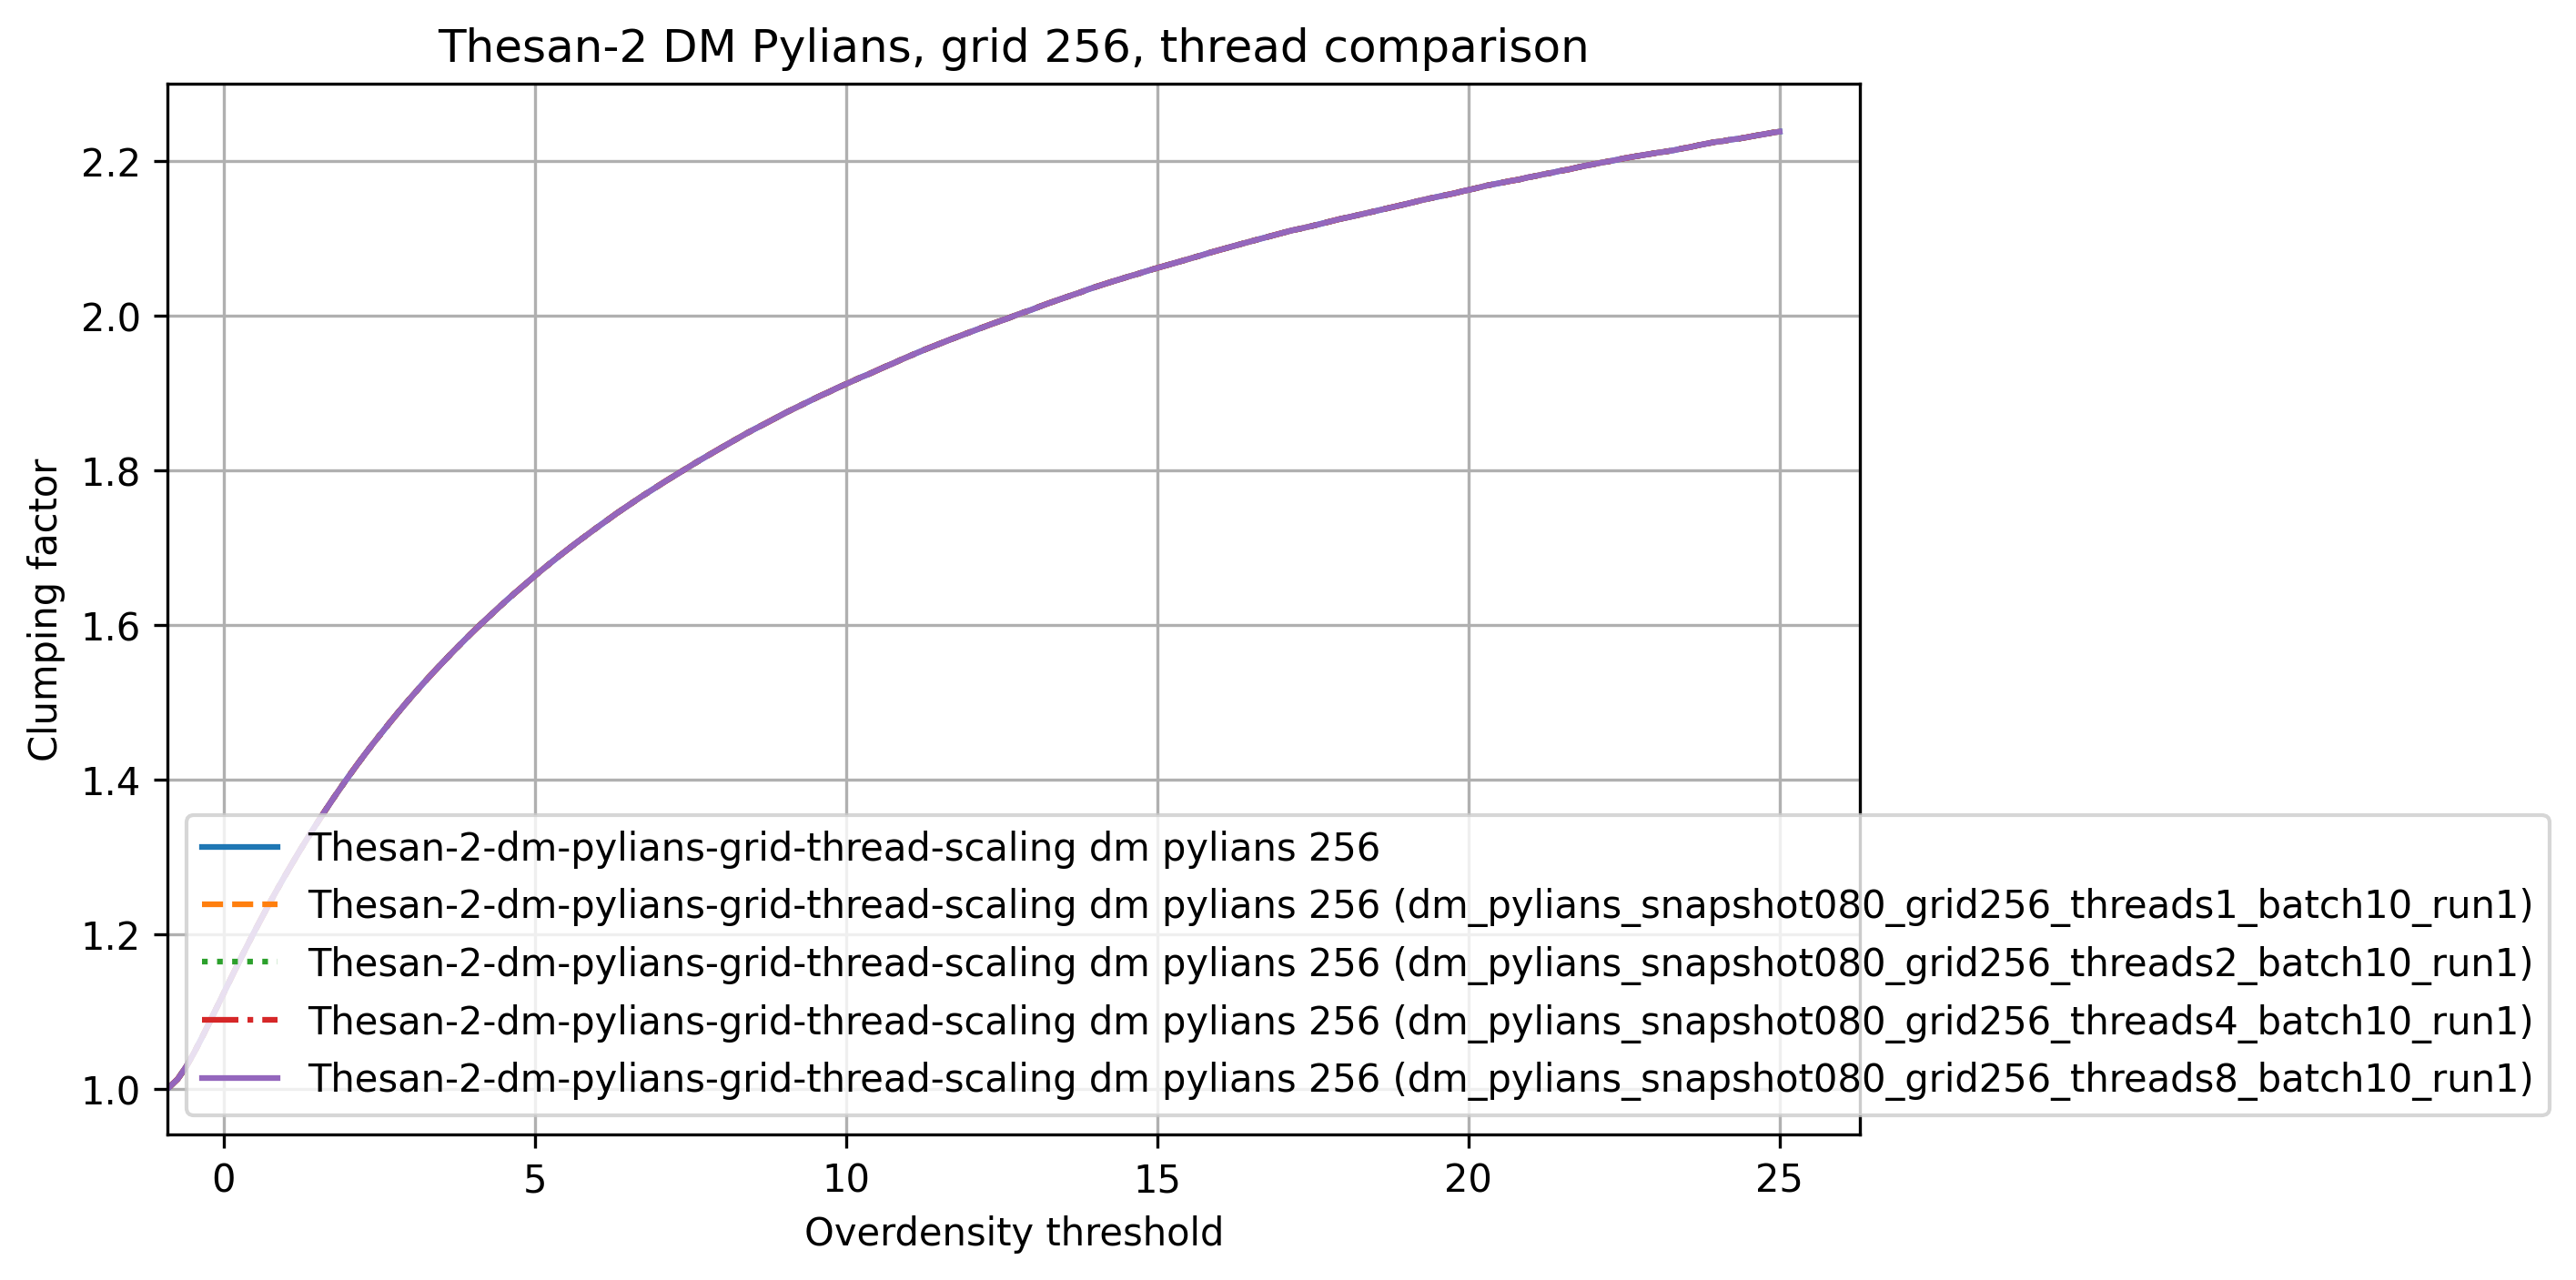
\includegraphics[width=\linewidth]{../results/analysis/operations/thesan/performance/combined/Thesan-2_dm_pylians_grid256_threads/analysis-94345f89284c/artifacts/Thesan-2_dm_pylians_grid256_threads.png}
    \caption{Existing Thesan-2 dark-matter Pylians clumping-factor curves for
    the available worker-count configurations at $256^3$.  The near-overlap
    of the curves provides a production-scale numerical-parity check.}
    \label{fig:parallel-worker-clumping}
\end{figure}

\begin{figure}[t]
    \centering
    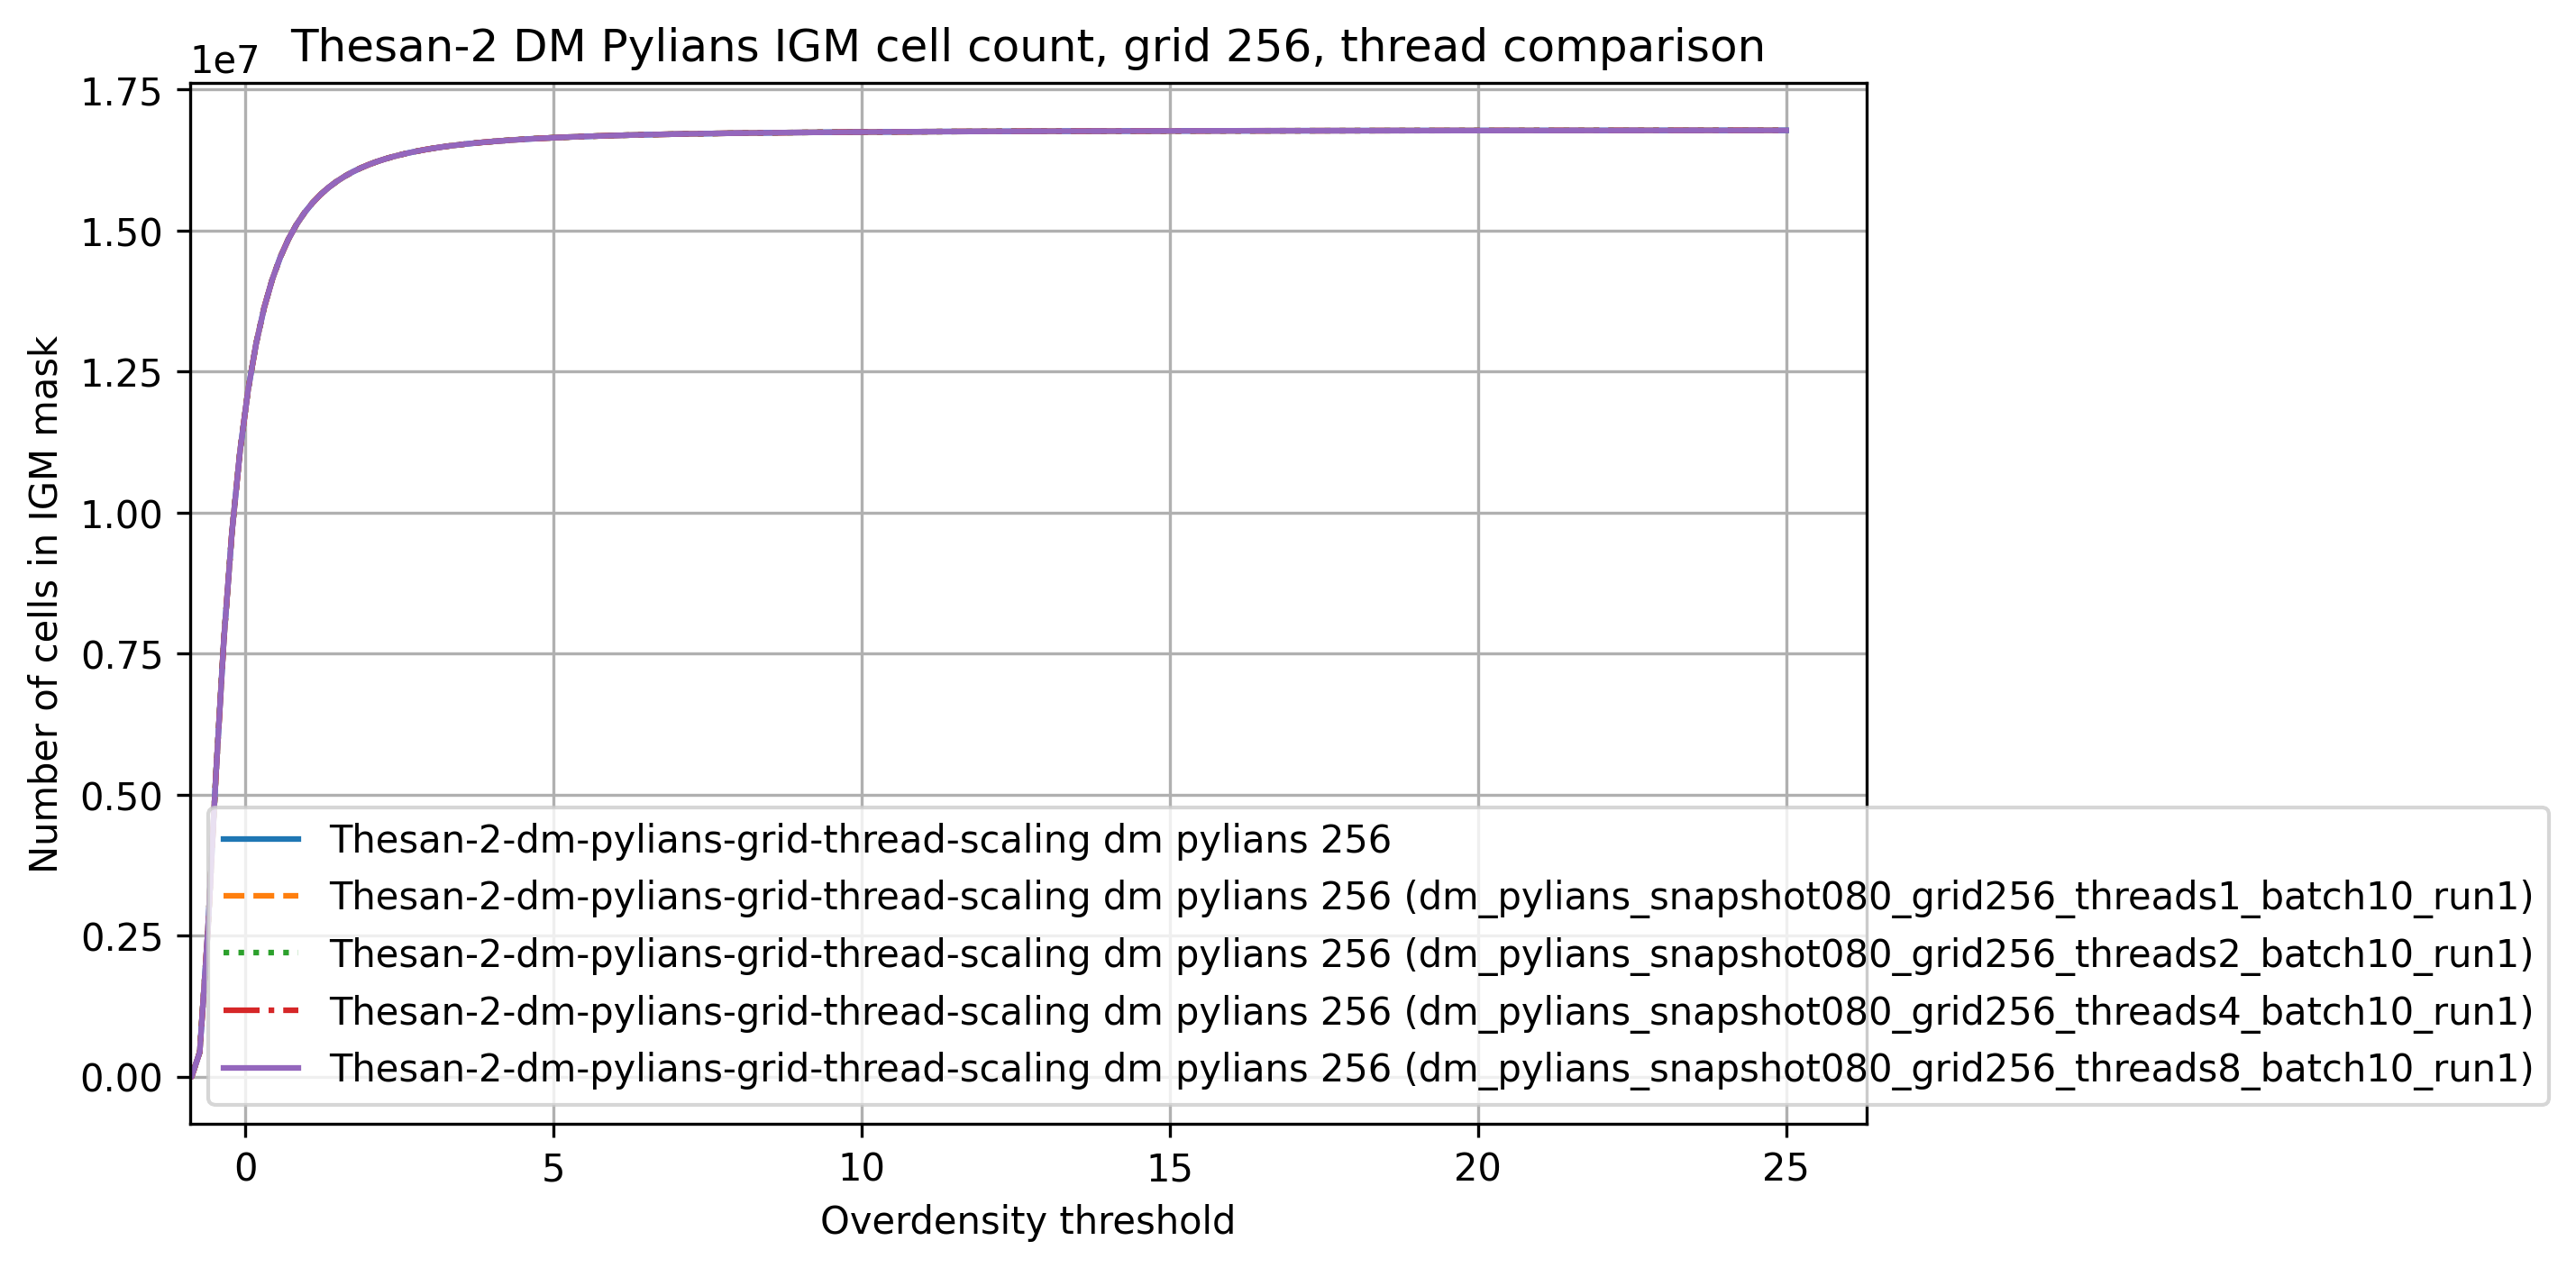
\includegraphics[width=\linewidth]{../results/analysis/operations/thesan/performance/combined/Thesan-2_dm_pylians_grid256_cell_counts/analysis-95b33b59128a/artifacts/Thesan-2_dm_pylians_grid256_cell_counts.png}
    \caption{Existing selected-cell-count diagnostic for the same worker
    configurations.  The overlap confirms that parallel execution does not
    change the IGM mask used by the clumping calculation.}
    \label{fig:parallel-worker-cells}
\end{figure}

\subsection{Benchmark evidence and protocol}

The repository contains 40 historical timing rows spanning Thesan-1 and
Thesan-2, $128^3$ through $1024^3$ grids, and requested worker counts from
one to sixteen.  These rows are retained as contextual evidence for grid
scaling and memory growth.  They are not used as the primary speedup claim:
the configurations contain a mixture of cache hits, lock waits, cache builds,
and one-off runs, and the raw JSON paths referenced by the consolidated CSV
are not all present after results consolidation.

The report-side extraction script named
reports/parallelization\_benchmark.py separates these historical
rows from controlled measurements and produces the compact summary figure in
Fig.~\ref{fig:parallel-benchmark}.  The controlled protocol requires only
six new grid computations on the machine containing the Thesan-2 snapshot:
snapshot 80, dark matter, Pylians, a $512^3$ grid, requested worker counts of
one and sixteen, and three alternating repeats at each setting.  The chunk
size, radius-bin batch size, partition mode, memory limit, software
environment, and node are fixed.  The summary cache is disabled or isolated
from previous runs.  Both requested and effective worker counts are recorded.

The primary timing statistic is the ratio of the median total time for the
serial runs to the median total time for the parallel runs.  The repeat range
and the grid-build timing are reported alongside this ratio.  If the six JSON
files are not available, the extraction script leaves the controlled panels
explicitly marked as pending and reports only the historical context; no
speedup is inferred from the contaminated historical timings.

\begin{figure*}[t]
    \centering
    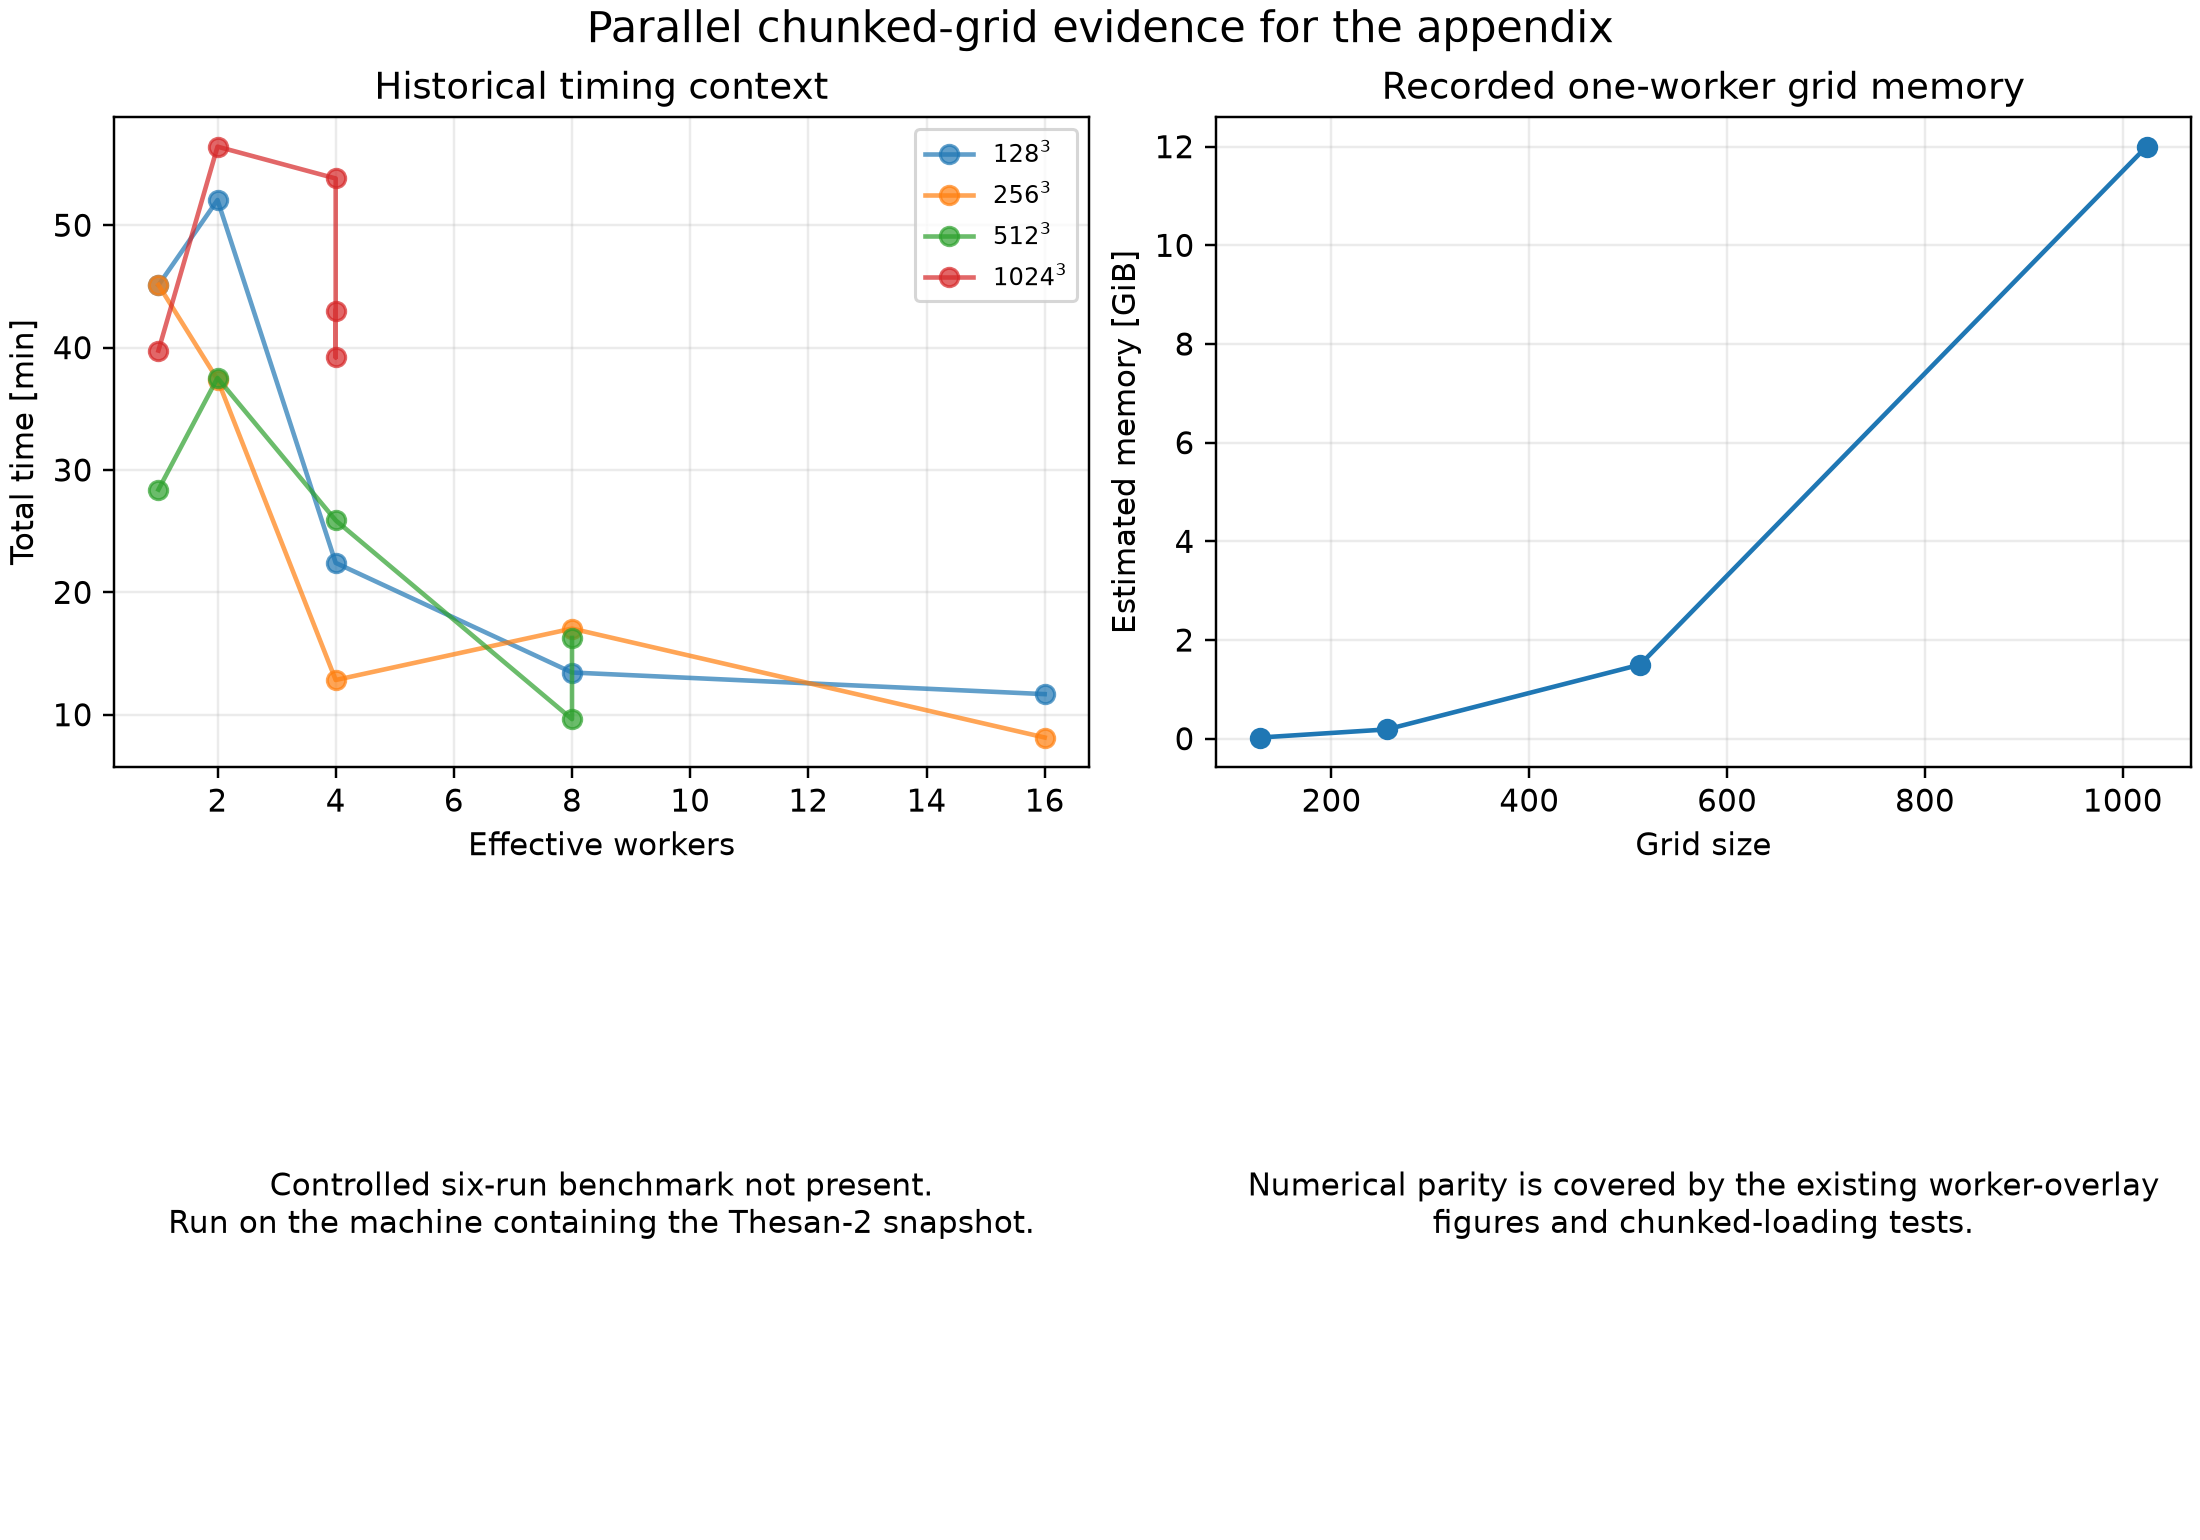
\includegraphics[width=0.96\textwidth]{figures/parallelization_benchmark.png}
    \caption{Compact evidence summary for the parallel chunked-grid path.
    The historical timing and memory panels are contextual.  The lower panels
    are populated from the six cache-isolated benchmark JSON files when they
    are available; otherwise they identify the missing controlled evidence
    rather than reporting an unsupported speedup.}
    \label{fig:parallel-benchmark}
\end{figure*}

\subsection{Limitations and reproducibility}

The controlled timing is a representative measurement of the process-pool
grid path, not a hardware-independent scaling law.  The effective worker
count can be lower than requested when the snapshot contains too few balanced
work units or when the memory policy applies a cap.  The appendix therefore
reports both counts and separates numerical parity from wall-clock behavior.
No new cosmological snapshots, particle fields, redshifts, or dark-matter
models are required for this validation: the existing scientific results and
worker overlays provide the broad numerical coverage, while the six
cache-isolated computations provide the only new timing evidence.



\end{document}
%
% ****** End of file apssamp.tex ******
